\documentclass{../config/paper}
\title{All TIKZ Figures}

\begin{document}



\begin{figure*}
\centering
% Created by tikzDevice version 0.12.3.1 on 2022-10-10 15:31:40
% !TEX encoding = UTF-8 Unicode
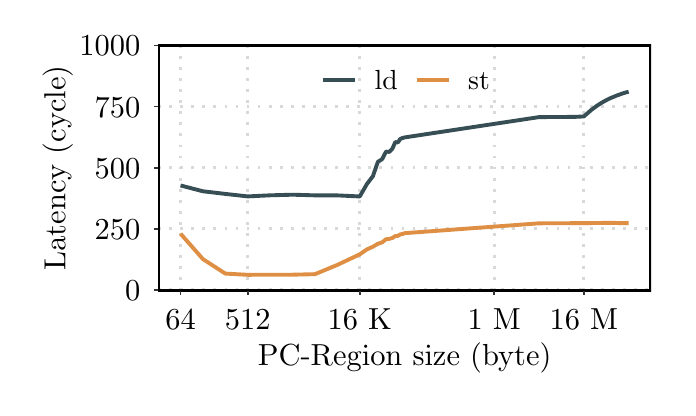
\begin{tikzpicture}[x=1pt,y=1pt]
\definecolor{fillColor}{RGB}{255,255,255}
\path[use as bounding box,fill=fillColor,fill opacity=0.00] (0,0) rectangle (231.26,130.09);
\begin{scope}
\path[clip] (  0.00,  0.00) rectangle (231.26,130.09);
\definecolor{drawColor}{RGB}{255,255,255}
\definecolor{fillColor}{RGB}{255,255,255}

\path[draw=drawColor,line width= 0.6pt,line join=round,line cap=round,fill=fillColor] (  0.00,  0.00) rectangle (231.26,130.09);
\end{scope}
\begin{scope}
\path[clip] ( 47.13, 34.85) rectangle (225.26,124.09);
\definecolor{fillColor}{RGB}{255,255,255}

\path[fill=fillColor] ( 47.13, 34.85) rectangle (225.26,124.09);
\definecolor{drawColor}{gray}{0.85}

\path[draw=drawColor,line width= 1.1pt,dash pattern=on 1pt off 3pt ,line join=round] ( 47.13, 35.29) --
	(225.26, 35.29);

\path[draw=drawColor,line width= 1.1pt,dash pattern=on 1pt off 3pt ,line join=round] ( 47.13, 57.38) --
	(225.26, 57.38);

\path[draw=drawColor,line width= 1.1pt,dash pattern=on 1pt off 3pt ,line join=round] ( 47.13, 79.47) --
	(225.26, 79.47);

\path[draw=drawColor,line width= 1.1pt,dash pattern=on 1pt off 3pt ,line join=round] ( 47.13,101.56) --
	(225.26,101.56);

\path[draw=drawColor,line width= 1.1pt,dash pattern=on 1pt off 3pt ,line join=round] ( 47.13,123.64) --
	(225.26,123.64);

\path[draw=drawColor,line width= 1.1pt,dash pattern=on 1pt off 3pt ,line join=round] ( 55.23, 34.85) --
	( 55.23,124.09);

\path[draw=drawColor,line width= 1.1pt,dash pattern=on 1pt off 3pt ,line join=round] ( 79.52, 34.85) --
	( 79.52,124.09);

\path[draw=drawColor,line width= 1.1pt,dash pattern=on 1pt off 3pt ,line join=round] (120.00, 34.85) --
	(120.00,124.09);

\path[draw=drawColor,line width= 1.1pt,dash pattern=on 1pt off 3pt ,line join=round] (168.59, 34.85) --
	(168.59,124.09);

\path[draw=drawColor,line width= 1.1pt,dash pattern=on 1pt off 3pt ,line join=round] (200.97, 34.85) --
	(200.97,124.09);
\definecolor{drawColor}{RGB}{223,143,68}

\path[draw=drawColor,line width= 1.4pt,line join=round] ( 55.23, 55.66) --
	( 63.33, 46.46) --
	( 71.42, 41.23) --
	( 79.52, 40.78) --
	( 87.62, 40.81) --
	( 95.71, 40.83) --
	(103.81, 41.02) --
	(111.91, 44.37) --
	(120.00, 48.19) --
	(122.61, 49.98) --
	(124.74, 50.93) --
	(126.54, 52.00) --
	(128.10, 52.52) --
	(129.48, 53.65) --
	(130.71, 53.79) --
	(131.82, 54.10) --
	(132.84, 54.81) --
	(133.77, 54.85) --
	(134.64, 55.41) --
	(135.44, 55.53) --
	(136.20, 55.83) --
	(184.78, 59.39) --
	(192.88, 59.42) --
	(197.61, 59.45) --
	(200.97, 59.46) --
	(203.58, 59.48) --
	(205.71, 59.51) --
	(207.51, 59.53) --
	(209.07, 59.56) --
	(210.45, 59.57) --
	(211.68, 59.55) --
	(212.79, 59.51) --
	(213.81, 59.46) --
	(214.74, 59.47) --
	(215.61, 59.47) --
	(216.41, 59.47) --
	(217.17, 59.45);
\definecolor{drawColor}{RGB}{55,78,85}

\path[draw=drawColor,line width= 1.4pt,line join=round] ( 55.23, 73.07) --
	( 63.33, 70.97) --
	( 71.42, 70.02) --
	( 79.52, 69.12) --
	( 87.62, 69.51) --
	( 95.71, 69.73) --
	(103.81, 69.50) --
	(111.91, 69.48) --
	(120.00, 69.10) --
	(122.61, 73.63) --
	(124.74, 76.41) --
	(126.54, 81.59) --
	(128.10, 82.60) --
	(129.48, 85.30) --
	(130.71, 85.20) --
	(131.82, 86.42) --
	(132.84, 88.77) --
	(133.77, 88.61) --
	(134.64, 89.90) --
	(135.44, 90.21) --
	(136.20, 90.43) --
	(184.78, 97.77) --
	(192.88, 97.82) --
	(197.61, 97.85) --
	(200.97, 98.01) --
	(203.58,100.29) --
	(205.71,101.88) --
	(207.51,103.02) --
	(209.07,103.88) --
	(210.45,104.57) --
	(211.68,105.08) --
	(212.79,105.54) --
	(213.81,105.89) --
	(214.74,106.25) --
	(215.61,106.52) --
	(216.41,106.75) --
	(217.17,106.93);
\definecolor{drawColor}{RGB}{0,0,0}

\path[draw=drawColor,line width= 1.7pt,line join=round,line cap=round] ( 47.13, 34.85) rectangle (225.26,124.09);
\end{scope}
\begin{scope}
\path[clip] (  0.00,  0.00) rectangle (231.26,130.09);
\definecolor{drawColor}{RGB}{0,0,0}

\node[text=drawColor,anchor=base east,inner sep=0pt, outer sep=0pt, scale=  1.10] at ( 40.71, 31.51) {0};

\node[text=drawColor,anchor=base east,inner sep=0pt, outer sep=0pt, scale=  1.10] at ( 40.71, 53.59) {250};

\node[text=drawColor,anchor=base east,inner sep=0pt, outer sep=0pt, scale=  1.10] at ( 40.71, 75.68) {500};

\node[text=drawColor,anchor=base east,inner sep=0pt, outer sep=0pt, scale=  1.10] at ( 40.71, 97.77) {750};

\node[text=drawColor,anchor=base east,inner sep=0pt, outer sep=0pt, scale=  1.10] at ( 40.71,119.86) {1000};
\end{scope}
\begin{scope}
\path[clip] (  0.00,  0.00) rectangle (231.26,130.09);
\definecolor{drawColor}{gray}{0.20}

\path[draw=drawColor,line width= 0.6pt,line join=round] ( 45.71, 35.29) --
	( 47.13, 35.29);

\path[draw=drawColor,line width= 0.6pt,line join=round] ( 45.71, 57.38) --
	( 47.13, 57.38);

\path[draw=drawColor,line width= 0.6pt,line join=round] ( 45.71, 79.47) --
	( 47.13, 79.47);

\path[draw=drawColor,line width= 0.6pt,line join=round] ( 45.71,101.56) --
	( 47.13,101.56);

\path[draw=drawColor,line width= 0.6pt,line join=round] ( 45.71,123.64) --
	( 47.13,123.64);
\end{scope}
\begin{scope}
\path[clip] (  0.00,  0.00) rectangle (231.26,130.09);
\definecolor{drawColor}{gray}{0.20}

\path[draw=drawColor,line width= 0.6pt,line join=round] ( 55.23, 33.43) --
	( 55.23, 34.85);

\path[draw=drawColor,line width= 0.6pt,line join=round] ( 79.52, 33.43) --
	( 79.52, 34.85);

\path[draw=drawColor,line width= 0.6pt,line join=round] (120.00, 33.43) --
	(120.00, 34.85);

\path[draw=drawColor,line width= 0.6pt,line join=round] (168.59, 33.43) --
	(168.59, 34.85);

\path[draw=drawColor,line width= 0.6pt,line join=round] (200.97, 33.43) --
	(200.97, 34.85);
\end{scope}
\begin{scope}
\path[clip] (  0.00,  0.00) rectangle (231.26,130.09);
\definecolor{drawColor}{RGB}{0,0,0}

\node[text=drawColor,anchor=base,inner sep=0pt, outer sep=0pt, scale=  1.10] at ( 55.23, 20.85) {64};

\node[text=drawColor,anchor=base,inner sep=0pt, outer sep=0pt, scale=  1.10] at ( 79.52, 20.85) {512};

\node[text=drawColor,anchor=base,inner sep=0pt, outer sep=0pt, scale=  1.10] at (120.00, 20.85) {16 K};

\node[text=drawColor,anchor=base,inner sep=0pt, outer sep=0pt, scale=  1.10] at (168.59, 20.85) {1 M};

\node[text=drawColor,anchor=base,inner sep=0pt, outer sep=0pt, scale=  1.10] at (200.97, 20.85) {16 M};
\end{scope}
\begin{scope}
\path[clip] (  0.00,  0.00) rectangle (231.26,130.09);
\definecolor{drawColor}{RGB}{0,0,0}

\node[text=drawColor,anchor=base,inner sep=0pt, outer sep=0pt, scale=  1.10] at (136.20,  8.14) {PC-Region size (byte)};
\end{scope}
\begin{scope}
\path[clip] (  0.00,  0.00) rectangle (231.26,130.09);
\definecolor{drawColor}{RGB}{0,0,0}

\node[text=drawColor,rotate= 90.00,anchor=base,inner sep=0pt, outer sep=0pt, scale=  1.10] at ( 13.58, 79.47) {Latency (cycle)};
\end{scope}
\begin{scope}
\path[clip] (  0.00,  0.00) rectangle (231.26,130.09);
\definecolor{drawColor}{RGB}{55,78,85}

\path[draw=drawColor,line width= 1.4pt,line join=round] (106.86,111.03) -- (118.42,111.03);
\end{scope}
\begin{scope}
\path[clip] (  0.00,  0.00) rectangle (231.26,130.09);
\definecolor{drawColor}{RGB}{55,78,85}

\path[draw=drawColor,line width= 1.4pt,line join=round] (106.86,111.03) -- (118.42,111.03);
\end{scope}
\begin{scope}
\path[clip] (  0.00,  0.00) rectangle (231.26,130.09);
\definecolor{drawColor}{RGB}{223,143,68}

\path[draw=drawColor,line width= 1.4pt,line join=round] (140.64,111.03) -- (152.21,111.03);
\end{scope}
\begin{scope}
\path[clip] (  0.00,  0.00) rectangle (231.26,130.09);
\definecolor{drawColor}{RGB}{223,143,68}

\path[draw=drawColor,line width= 1.4pt,line join=round] (140.64,111.03) -- (152.21,111.03);
\end{scope}
\begin{scope}
\path[clip] (  0.00,  0.00) rectangle (231.26,130.09);
\definecolor{drawColor}{RGB}{0,0,0}

\node[text=drawColor,anchor=base west,inner sep=0pt, outer sep=0pt, scale=  1.00] at (125.37,107.59) {ld};
\end{scope}
\begin{scope}
\path[clip] (  0.00,  0.00) rectangle (231.26,130.09);
\definecolor{drawColor}{RGB}{0,0,0}

\node[text=drawColor,anchor=base west,inner sep=0pt, outer sep=0pt, scale=  1.00] at (159.15,107.59) {st};
\end{scope}
\end{tikzpicture}

\caption{plot/reference/fig2a-pointer-chasing.tikz}
\end{figure*}


\begin{figure*}
\centering
% Created by tikzDevice version 0.12.3.1 on 2022-10-11 00:41:49
% !TEX encoding = UTF-8 Unicode
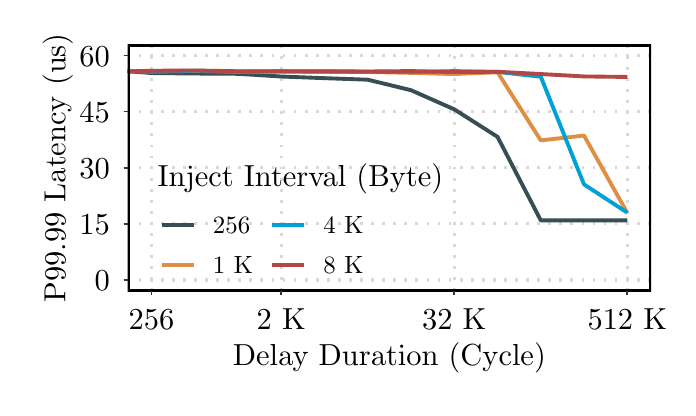
\begin{tikzpicture}[x=1pt,y=1pt]
\definecolor{fillColor}{RGB}{255,255,255}
\path[use as bounding box,fill=fillColor,fill opacity=0.00] (0,0) rectangle (231.26,130.09);
\begin{scope}
\path[clip] (  0.00,  0.00) rectangle (231.26,130.09);
\definecolor{drawColor}{RGB}{255,255,255}
\definecolor{fillColor}{RGB}{255,255,255}

\path[draw=drawColor,line width= 0.6pt,line join=round,line cap=round,fill=fillColor] (  0.00,  0.00) rectangle (231.26,130.09);
\end{scope}
\begin{scope}
\path[clip] ( 36.13, 34.85) rectangle (225.26,124.09);
\definecolor{fillColor}{RGB}{255,255,255}

\path[fill=fillColor] ( 36.13, 34.85) rectangle (225.26,124.09);
\definecolor{drawColor}{gray}{0.85}

\path[draw=drawColor,line width= 1.1pt,dash pattern=on 1pt off 3pt ,line join=round] ( 36.13, 38.91) --
	(225.26, 38.91);

\path[draw=drawColor,line width= 1.1pt,dash pattern=on 1pt off 3pt ,line join=round] ( 36.13, 59.19) --
	(225.26, 59.19);

\path[draw=drawColor,line width= 1.1pt,dash pattern=on 1pt off 3pt ,line join=round] ( 36.13, 79.47) --
	(225.26, 79.47);

\path[draw=drawColor,line width= 1.1pt,dash pattern=on 1pt off 3pt ,line join=round] ( 36.13, 99.75) --
	(225.26, 99.75);

\path[draw=drawColor,line width= 1.1pt,dash pattern=on 1pt off 3pt ,line join=round] ( 36.13,120.03) --
	(225.26,120.03);

\path[draw=drawColor,line width= 1.1pt,dash pattern=on 1pt off 3pt ,line join=round] ( 44.73, 34.85) --
	( 44.73,124.09);

\path[draw=drawColor,line width= 1.1pt,dash pattern=on 1pt off 3pt ,line join=round] ( 91.62, 34.85) --
	( 91.62,124.09);

\path[draw=drawColor,line width= 1.1pt,dash pattern=on 1pt off 3pt ,line join=round] (154.14, 34.85) --
	(154.14,124.09);

\path[draw=drawColor,line width= 1.1pt,dash pattern=on 1pt off 3pt ,line join=round] (216.67, 34.85) --
	(216.67,124.09);
\definecolor{drawColor}{RGB}{55,78,85}

\path[draw=drawColor,line width= 1.4pt,line join=round] ( 36.13,114.36) --
	( 44.73,113.69) --
	( 60.36,113.52) --
	( 75.99,113.41) --
	( 91.62,112.44) --
	(107.25,111.84) --
	(122.88,111.29) --
	(138.51,107.50) --
	(154.14,100.58) --
	(169.78, 90.63) --
	(185.41, 60.46) --
	(201.04, 60.45) --
	(216.67, 60.46);
\definecolor{drawColor}{RGB}{223,143,68}

\path[draw=drawColor,line width= 1.4pt,line join=round] ( 36.13,114.45) --
	( 44.73,114.24) --
	( 60.36,114.47) --
	( 75.99,114.18) --
	( 91.62,114.20) --
	(107.25,114.08) --
	(122.88,114.10) --
	(138.51,113.76) --
	(154.14,113.32) --
	(169.78,113.98) --
	(185.41, 89.36) --
	(201.04, 91.10) --
	(216.67, 63.15);
\definecolor{drawColor}{RGB}{0,161,213}

\path[draw=drawColor,line width= 1.4pt,line join=round] ( 36.13,114.32) --
	( 44.73,114.30) --
	( 60.36,114.54) --
	( 75.99,114.19) --
	( 91.62,114.30) --
	(107.25,114.31) --
	(122.88,114.16) --
	(138.51,114.05) --
	(154.14,114.40) --
	(169.78,114.10) --
	(185.41,112.36) --
	(201.04, 73.44) --
	(216.67, 63.25);
\definecolor{drawColor}{RGB}{178,71,69}

\path[draw=drawColor,line width= 1.4pt,line join=round] ( 36.13,114.26) --
	( 44.73,114.52) --
	( 60.36,114.62) --
	( 75.99,114.34) --
	( 91.62,114.34) --
	(107.25,114.33) --
	(122.88,114.25) --
	(138.51,114.40) --
	(154.14,114.05) --
	(169.78,114.16) --
	(185.41,113.33) --
	(201.04,112.47) --
	(216.67,112.28);
\definecolor{drawColor}{RGB}{0,0,0}

\path[draw=drawColor,line width= 1.7pt,line join=round,line cap=round] ( 36.13, 34.85) rectangle (225.26,124.09);
\end{scope}
\begin{scope}
\path[clip] (  0.00,  0.00) rectangle (231.26,130.09);
\definecolor{drawColor}{RGB}{0,0,0}

\node[text=drawColor,anchor=base east,inner sep=0pt, outer sep=0pt, scale=  1.10] at ( 29.71, 35.12) {0};

\node[text=drawColor,anchor=base east,inner sep=0pt, outer sep=0pt, scale=  1.10] at ( 29.71, 55.40) {15};

\node[text=drawColor,anchor=base east,inner sep=0pt, outer sep=0pt, scale=  1.10] at ( 29.71, 75.68) {30};

\node[text=drawColor,anchor=base east,inner sep=0pt, outer sep=0pt, scale=  1.10] at ( 29.71, 95.96) {45};

\node[text=drawColor,anchor=base east,inner sep=0pt, outer sep=0pt, scale=  1.10] at ( 29.71,116.24) {60};
\end{scope}
\begin{scope}
\path[clip] (  0.00,  0.00) rectangle (231.26,130.09);
\definecolor{drawColor}{gray}{0.20}

\path[draw=drawColor,line width= 0.6pt,line join=round] ( 34.71, 38.91) --
	( 36.13, 38.91);

\path[draw=drawColor,line width= 0.6pt,line join=round] ( 34.71, 59.19) --
	( 36.13, 59.19);

\path[draw=drawColor,line width= 0.6pt,line join=round] ( 34.71, 79.47) --
	( 36.13, 79.47);

\path[draw=drawColor,line width= 0.6pt,line join=round] ( 34.71, 99.75) --
	( 36.13, 99.75);

\path[draw=drawColor,line width= 0.6pt,line join=round] ( 34.71,120.03) --
	( 36.13,120.03);
\end{scope}
\begin{scope}
\path[clip] (  0.00,  0.00) rectangle (231.26,130.09);
\definecolor{drawColor}{gray}{0.20}

\path[draw=drawColor,line width= 0.6pt,line join=round] ( 44.73, 33.43) --
	( 44.73, 34.85);

\path[draw=drawColor,line width= 0.6pt,line join=round] ( 91.62, 33.43) --
	( 91.62, 34.85);

\path[draw=drawColor,line width= 0.6pt,line join=round] (154.14, 33.43) --
	(154.14, 34.85);

\path[draw=drawColor,line width= 0.6pt,line join=round] (216.67, 33.43) --
	(216.67, 34.85);
\end{scope}
\begin{scope}
\path[clip] (  0.00,  0.00) rectangle (231.26,130.09);
\definecolor{drawColor}{RGB}{0,0,0}

\node[text=drawColor,anchor=base,inner sep=0pt, outer sep=0pt, scale=  1.10] at ( 44.73, 20.85) {256};

\node[text=drawColor,anchor=base,inner sep=0pt, outer sep=0pt, scale=  1.10] at ( 91.62, 20.85) {2 K};

\node[text=drawColor,anchor=base,inner sep=0pt, outer sep=0pt, scale=  1.10] at (154.14, 20.85) {32 K};

\node[text=drawColor,anchor=base,inner sep=0pt, outer sep=0pt, scale=  1.10] at (216.67, 20.85) {512 K};
\end{scope}
\begin{scope}
\path[clip] (  0.00,  0.00) rectangle (231.26,130.09);
\definecolor{drawColor}{RGB}{0,0,0}

\node[text=drawColor,anchor=base,inner sep=0pt, outer sep=0pt, scale=  1.10] at (130.70,  8.14) {Delay Duration (Cycle)};
\end{scope}
\begin{scope}
\path[clip] (  0.00,  0.00) rectangle (231.26,130.09);
\definecolor{drawColor}{RGB}{0,0,0}

\node[text=drawColor,rotate= 90.00,anchor=base,inner sep=0pt, outer sep=0pt, scale=  1.10] at ( 13.58, 79.47) {P99.99 Latency (us)};
\end{scope}
\begin{scope}
\path[clip] (  0.00,  0.00) rectangle (231.26,130.09);
\definecolor{drawColor}{RGB}{0,0,0}

\node[text=drawColor,anchor=base west,inner sep=0pt, outer sep=0pt, scale=  1.10] at ( 46.98, 72.71) {Inject Interval (Byte)};
\end{scope}
\begin{scope}
\path[clip] (  0.00,  0.00) rectangle (231.26,130.09);
\definecolor{drawColor}{RGB}{55,78,85}

\path[draw=drawColor,line width= 1.4pt,line join=round] ( 48.43, 58.92) -- ( 59.99, 58.92);
\end{scope}
\begin{scope}
\path[clip] (  0.00,  0.00) rectangle (231.26,130.09);
\definecolor{drawColor}{RGB}{223,143,68}

\path[draw=drawColor,line width= 1.4pt,line join=round] ( 48.43, 44.46) -- ( 59.99, 44.46);
\end{scope}
\begin{scope}
\path[clip] (  0.00,  0.00) rectangle (231.26,130.09);
\definecolor{drawColor}{RGB}{0,161,213}

\path[draw=drawColor,line width= 1.4pt,line join=round] ( 88.38, 58.92) -- ( 99.94, 58.92);
\end{scope}
\begin{scope}
\path[clip] (  0.00,  0.00) rectangle (231.26,130.09);
\definecolor{drawColor}{RGB}{178,71,69}

\path[draw=drawColor,line width= 1.4pt,line join=round] ( 88.38, 44.46) -- ( 99.94, 44.46);
\end{scope}
\begin{scope}
\path[clip] (  0.00,  0.00) rectangle (231.26,130.09);
\definecolor{drawColor}{RGB}{0,0,0}

\node[text=drawColor,anchor=base west,inner sep=0pt, outer sep=0pt, scale=  0.90] at ( 66.94, 55.82) {256};
\end{scope}
\begin{scope}
\path[clip] (  0.00,  0.00) rectangle (231.26,130.09);
\definecolor{drawColor}{RGB}{0,0,0}

\node[text=drawColor,anchor=base west,inner sep=0pt, outer sep=0pt, scale=  0.90] at ( 66.94, 41.37) {1 K};
\end{scope}
\begin{scope}
\path[clip] (  0.00,  0.00) rectangle (231.26,130.09);
\definecolor{drawColor}{RGB}{0,0,0}

\node[text=drawColor,anchor=base west,inner sep=0pt, outer sep=0pt, scale=  0.90] at (106.89, 55.82) {4 K};
\end{scope}
\begin{scope}
\path[clip] (  0.00,  0.00) rectangle (231.26,130.09);
\definecolor{drawColor}{RGB}{0,0,0}

\node[text=drawColor,anchor=base west,inner sep=0pt, outer sep=0pt, scale=  0.90] at (106.89, 41.37) {8 K};
\end{scope}
\end{tikzpicture}

\caption{plot/reference/fig5b-overwrite-delay-p99-latency-sample.tikz}
\end{figure*}


\begin{figure*}
\centering
% Created by tikzDevice version 0.12.3.1 on 2022-10-11 15:27:34
% !TEX encoding = UTF-8 Unicode
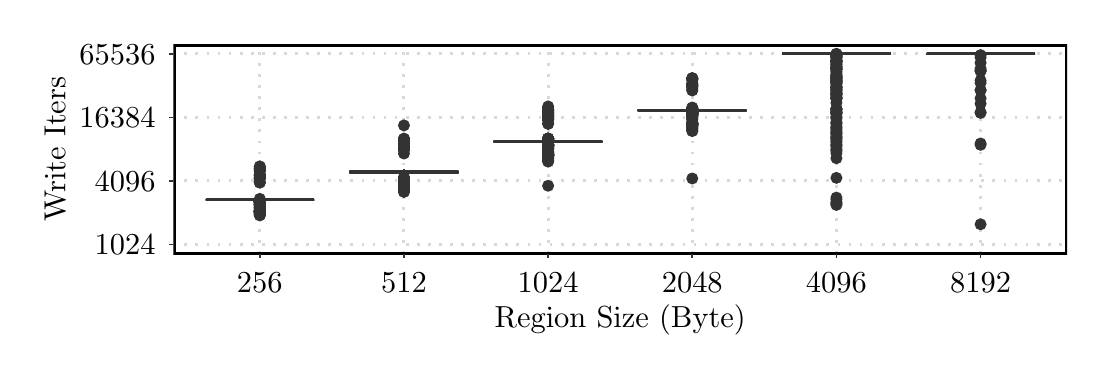
\begin{tikzpicture}[x=1pt,y=1pt]
\definecolor{fillColor}{RGB}{255,255,255}
\path[use as bounding box,fill=fillColor,fill opacity=0.00] (0,0) rectangle (381.59,116.64);
\begin{scope}
\path[clip] (  0.00,  0.00) rectangle (381.59,116.64);
\definecolor{drawColor}{RGB}{255,255,255}
\definecolor{fillColor}{RGB}{255,255,255}

\path[draw=drawColor,line width= 0.6pt,line join=round,line cap=round,fill=fillColor] (  0.00,  0.00) rectangle (381.59,116.64);
\end{scope}
\begin{scope}
\path[clip] ( 52.63, 34.85) rectangle (375.59,110.64);
\definecolor{fillColor}{RGB}{255,255,255}

\path[fill=fillColor] ( 52.63, 34.85) rectangle (375.59,110.64);
\definecolor{drawColor}{gray}{0.85}

\path[draw=drawColor,line width= 1.1pt,dash pattern=on 1pt off 3pt ,line join=round] ( 52.63, 38.30) --
	(375.59, 38.30);

\path[draw=drawColor,line width= 1.1pt,dash pattern=on 1pt off 3pt ,line join=round] ( 52.63, 61.26) --
	(375.59, 61.26);

\path[draw=drawColor,line width= 1.1pt,dash pattern=on 1pt off 3pt ,line join=round] ( 52.63, 84.23) --
	(375.59, 84.23);

\path[draw=drawColor,line width= 1.1pt,dash pattern=on 1pt off 3pt ,line join=round] ( 52.63,107.20) --
	(375.59,107.20);

\path[draw=drawColor,line width= 1.1pt,dash pattern=on 1pt off 3pt ,line join=round] ( 83.88, 34.85) --
	( 83.88,110.64);

\path[draw=drawColor,line width= 1.1pt,dash pattern=on 1pt off 3pt ,line join=round] (135.97, 34.85) --
	(135.97,110.64);

\path[draw=drawColor,line width= 1.1pt,dash pattern=on 1pt off 3pt ,line join=round] (188.06, 34.85) --
	(188.06,110.64);

\path[draw=drawColor,line width= 1.1pt,dash pattern=on 1pt off 3pt ,line join=round] (240.15, 34.85) --
	(240.15,110.64);

\path[draw=drawColor,line width= 1.1pt,dash pattern=on 1pt off 3pt ,line join=round] (292.24, 34.85) --
	(292.24,110.64);

\path[draw=drawColor,line width= 1.1pt,dash pattern=on 1pt off 3pt ,line join=round] (344.33, 34.85) --
	(344.33,110.64);
\definecolor{drawColor}{gray}{0.20}
\definecolor{fillColor}{gray}{0.20}

\path[draw=drawColor,line width= 0.4pt,line join=round,line cap=round,fill=fillColor] ( 83.88, 49.58) circle (  1.96);

\path[draw=drawColor,line width= 0.4pt,line join=round,line cap=round,fill=fillColor] ( 83.88, 53.65) circle (  1.96);

\path[draw=drawColor,line width= 0.4pt,line join=round,line cap=round,fill=fillColor] ( 83.88, 51.81) circle (  1.96);

\path[draw=drawColor,line width= 0.4pt,line join=round,line cap=round,fill=fillColor] ( 83.88, 52.65) circle (  1.96);

\path[draw=drawColor,line width= 0.4pt,line join=round,line cap=round,fill=fillColor] ( 83.88, 50.08) circle (  1.96);

\path[draw=drawColor,line width= 0.4pt,line join=round,line cap=round,fill=fillColor] ( 83.88, 53.96) circle (  1.96);

\path[draw=drawColor,line width= 0.4pt,line join=round,line cap=round,fill=fillColor] ( 83.88, 51.64) circle (  1.96);

\path[draw=drawColor,line width= 0.4pt,line join=round,line cap=round,fill=fillColor] ( 83.88, 53.95) circle (  1.96);

\path[draw=drawColor,line width= 0.4pt,line join=round,line cap=round,fill=fillColor] ( 83.88, 53.94) circle (  1.96);

\path[draw=drawColor,line width= 0.4pt,line join=round,line cap=round,fill=fillColor] ( 83.88, 53.99) circle (  1.96);

\path[draw=drawColor,line width= 0.4pt,line join=round,line cap=round,fill=fillColor] ( 83.88, 50.36) circle (  1.96);

\path[draw=drawColor,line width= 0.4pt,line join=round,line cap=round,fill=fillColor] ( 83.88, 51.64) circle (  1.96);

\path[draw=drawColor,line width= 0.4pt,line join=round,line cap=round,fill=fillColor] ( 83.88, 53.98) circle (  1.96);

\path[draw=drawColor,line width= 0.4pt,line join=round,line cap=round,fill=fillColor] ( 83.88, 53.87) circle (  1.96);

\path[draw=drawColor,line width= 0.4pt,line join=round,line cap=round,fill=fillColor] ( 83.88, 53.97) circle (  1.96);

\path[draw=drawColor,line width= 0.4pt,line join=round,line cap=round,fill=fillColor] ( 83.88, 49.92) circle (  1.96);

\path[draw=drawColor,line width= 0.4pt,line join=round,line cap=round,fill=fillColor] ( 83.88, 60.81) circle (  1.96);

\path[draw=drawColor,line width= 0.4pt,line join=round,line cap=round,fill=fillColor] ( 83.88, 62.09) circle (  1.96);

\path[draw=drawColor,line width= 0.4pt,line join=round,line cap=round,fill=fillColor] ( 83.88, 66.52) circle (  1.96);

\path[draw=drawColor,line width= 0.4pt,line join=round,line cap=round,fill=fillColor] ( 83.88, 64.93) circle (  1.96);

\path[draw=drawColor,line width= 0.4pt,line join=round,line cap=round,fill=fillColor] ( 83.88, 53.68) circle (  1.96);

\path[draw=drawColor,line width= 0.4pt,line join=round,line cap=round,fill=fillColor] ( 83.88, 53.55) circle (  1.96);

\path[draw=drawColor,line width= 0.4pt,line join=round,line cap=round,fill=fillColor] ( 83.88, 49.98) circle (  1.96);

\path[draw=drawColor,line width= 0.4pt,line join=round,line cap=round,fill=fillColor] ( 83.88, 53.97) circle (  1.96);

\path[draw=drawColor,line width= 0.4pt,line join=round,line cap=round,fill=fillColor] ( 83.88, 50.27) circle (  1.96);

\path[draw=drawColor,line width= 0.4pt,line join=round,line cap=round,fill=fillColor] ( 83.88, 49.14) circle (  1.96);

\path[draw=drawColor,line width= 0.4pt,line join=round,line cap=round,fill=fillColor] ( 83.88, 50.49) circle (  1.96);

\path[draw=drawColor,line width= 0.4pt,line join=round,line cap=round,fill=fillColor] ( 83.88, 51.21) circle (  1.96);

\path[draw=drawColor,line width= 0.4pt,line join=round,line cap=round,fill=fillColor] ( 83.88, 52.57) circle (  1.96);

\path[draw=drawColor,line width= 0.4pt,line join=round,line cap=round,fill=fillColor] ( 83.88, 62.32) circle (  1.96);

\path[draw=drawColor,line width= 0.4pt,line join=round,line cap=round,fill=fillColor] ( 83.88, 51.68) circle (  1.96);

\path[draw=drawColor,line width= 0.4pt,line join=round,line cap=round,fill=fillColor] ( 83.88, 53.55) circle (  1.96);

\path[draw=drawColor,line width= 0.4pt,line join=round,line cap=round,fill=fillColor] ( 83.88, 53.84) circle (  1.96);

\path[draw=drawColor,line width= 0.4pt,line join=round,line cap=round,fill=fillColor] ( 83.88, 53.79) circle (  1.96);

\path[draw=drawColor,line width= 0.4pt,line join=round,line cap=round,fill=fillColor] ( 83.88, 50.65) circle (  1.96);

\path[draw=drawColor,line width= 0.4pt,line join=round,line cap=round,fill=fillColor] ( 83.88, 53.67) circle (  1.96);

\path[draw=drawColor,line width= 0.4pt,line join=round,line cap=round,fill=fillColor] ( 83.88, 62.17) circle (  1.96);

\path[draw=drawColor,line width= 0.4pt,line join=round,line cap=round,fill=fillColor] ( 83.88, 64.95) circle (  1.96);

\path[draw=drawColor,line width= 0.4pt,line join=round,line cap=round,fill=fillColor] ( 83.88, 50.34) circle (  1.96);

\path[draw=drawColor,line width= 0.4pt,line join=round,line cap=round,fill=fillColor] ( 83.88, 54.01) circle (  1.96);

\path[draw=drawColor,line width= 0.4pt,line join=round,line cap=round,fill=fillColor] ( 83.88, 63.09) circle (  1.96);

\path[draw=drawColor,line width= 0.4pt,line join=round,line cap=round,fill=fillColor] ( 83.88, 53.35) circle (  1.96);

\path[draw=drawColor,line width= 0.4pt,line join=round,line cap=round,fill=fillColor] ( 83.88, 53.95) circle (  1.96);

\path[draw=drawColor,line width= 0.4pt,line join=round,line cap=round,fill=fillColor] ( 83.88, 53.68) circle (  1.96);

\path[draw=drawColor,line width= 0.4pt,line join=round,line cap=round,fill=fillColor] ( 83.88, 53.99) circle (  1.96);

\path[draw=drawColor,line width= 0.4pt,line join=round,line cap=round,fill=fillColor] ( 83.88, 50.17) circle (  1.96);

\path[draw=drawColor,line width= 0.4pt,line join=round,line cap=round,fill=fillColor] ( 83.88, 51.95) circle (  1.96);

\path[draw=drawColor,line width= 0.4pt,line join=round,line cap=round,fill=fillColor] ( 83.88, 63.48) circle (  1.96);

\path[draw=drawColor,line width= 0.4pt,line join=round,line cap=round,fill=fillColor] ( 83.88, 50.12) circle (  1.96);

\path[draw=drawColor,line width= 0.4pt,line join=round,line cap=round,fill=fillColor] ( 83.88, 51.12) circle (  1.96);

\path[draw=drawColor,line width= 0.4pt,line join=round,line cap=round,fill=fillColor] ( 83.88, 50.08) circle (  1.96);

\path[draw=drawColor,line width= 0.4pt,line join=round,line cap=round,fill=fillColor] ( 83.88, 50.35) circle (  1.96);

\path[draw=drawColor,line width= 0.4pt,line join=round,line cap=round,fill=fillColor] ( 83.88, 53.97) circle (  1.96);

\path[draw=drawColor,line width= 0.4pt,line join=round,line cap=round,fill=fillColor] ( 83.88, 53.67) circle (  1.96);

\path[draw=drawColor,line width= 0.4pt,line join=round,line cap=round,fill=fillColor] ( 83.88, 52.55) circle (  1.96);

\path[draw=drawColor,line width= 0.4pt,line join=round,line cap=round,fill=fillColor] ( 83.88, 52.76) circle (  1.96);

\path[draw=drawColor,line width= 0.4pt,line join=round,line cap=round,fill=fillColor] ( 83.88, 66.32) circle (  1.96);

\path[draw=drawColor,line width= 0.4pt,line join=round,line cap=round,fill=fillColor] ( 83.88, 49.12) circle (  1.96);

\path[draw=drawColor,line width= 0.4pt,line join=round,line cap=round,fill=fillColor] ( 83.88, 54.00) circle (  1.96);

\path[draw=drawColor,line width= 0.4pt,line join=round,line cap=round,fill=fillColor] ( 83.88, 53.97) circle (  1.96);

\path[draw=drawColor,line width= 0.4pt,line join=round,line cap=round,fill=fillColor] ( 83.88, 66.39) circle (  1.96);

\path[draw=drawColor,line width= 0.4pt,line join=round,line cap=round,fill=fillColor] ( 83.88, 50.42) circle (  1.96);

\path[draw=drawColor,line width= 0.4pt,line join=round,line cap=round,fill=fillColor] ( 83.88, 53.31) circle (  1.96);

\path[draw=drawColor,line width= 0.4pt,line join=round,line cap=round,fill=fillColor] ( 83.88, 52.59) circle (  1.96);

\path[draw=drawColor,line width= 0.4pt,line join=round,line cap=round,fill=fillColor] ( 83.88, 52.72) circle (  1.96);

\path[draw=drawColor,line width= 0.4pt,line join=round,line cap=round,fill=fillColor] ( 83.88, 48.80) circle (  1.96);

\path[draw=drawColor,line width= 0.4pt,line join=round,line cap=round,fill=fillColor] ( 83.88, 65.80) circle (  1.96);

\path[draw=drawColor,line width= 0.4pt,line join=round,line cap=round,fill=fillColor] ( 83.88, 53.68) circle (  1.96);

\path[draw=drawColor,line width= 0.4pt,line join=round,line cap=round,fill=fillColor] ( 83.88, 53.93) circle (  1.96);

\path[draw=drawColor,line width= 0.4pt,line join=round,line cap=round,fill=fillColor] ( 83.88, 50.23) circle (  1.96);

\path[draw=drawColor,line width= 0.4pt,line join=round,line cap=round,fill=fillColor] ( 83.88, 53.89) circle (  1.96);

\path[draw=drawColor,line width= 0.4pt,line join=round,line cap=round,fill=fillColor] ( 83.88, 53.96) circle (  1.96);

\path[draw=drawColor,line width= 0.4pt,line join=round,line cap=round,fill=fillColor] ( 83.88, 53.99) circle (  1.96);

\path[draw=drawColor,line width= 0.4pt,line join=round,line cap=round,fill=fillColor] ( 83.88, 54.00) circle (  1.96);

\path[draw=drawColor,line width= 0.4pt,line join=round,line cap=round,fill=fillColor] ( 83.88, 53.96) circle (  1.96);

\path[draw=drawColor,line width= 0.4pt,line join=round,line cap=round,fill=fillColor] ( 83.88, 50.16) circle (  1.96);

\path[draw=drawColor,line width= 0.4pt,line join=round,line cap=round,fill=fillColor] ( 83.88, 50.83) circle (  1.96);

\path[draw=drawColor,line width= 0.4pt,line join=round,line cap=round,fill=fillColor] ( 83.88, 49.94) circle (  1.96);

\path[draw=drawColor,line width= 0.4pt,line join=round,line cap=round,fill=fillColor] ( 83.88, 50.40) circle (  1.96);

\path[draw=drawColor,line width= 0.4pt,line join=round,line cap=round,fill=fillColor] ( 83.88, 49.96) circle (  1.96);

\path[draw=drawColor,line width= 0.4pt,line join=round,line cap=round,fill=fillColor] ( 83.88, 53.91) circle (  1.96);

\path[draw=drawColor,line width= 0.4pt,line join=round,line cap=round,fill=fillColor] ( 83.88, 60.66) circle (  1.96);

\path[draw=drawColor,line width= 0.4pt,line join=round,line cap=round,fill=fillColor] ( 83.88, 52.62) circle (  1.96);

\path[draw=drawColor,line width= 0.4pt,line join=round,line cap=round,fill=fillColor] ( 83.88, 53.41) circle (  1.96);

\path[draw=drawColor,line width= 0.4pt,line join=round,line cap=round,fill=fillColor] ( 83.88, 52.66) circle (  1.96);

\path[draw=drawColor,line width= 0.4pt,line join=round,line cap=round,fill=fillColor] ( 83.88, 65.67) circle (  1.96);

\path[draw=drawColor,line width= 0.4pt,line join=round,line cap=round,fill=fillColor] ( 83.88, 49.94) circle (  1.96);

\path[draw=drawColor,line width= 0.4pt,line join=round,line cap=round,fill=fillColor] ( 83.88, 53.79) circle (  1.96);

\path[draw=drawColor,line width= 0.4pt,line join=round,line cap=round,fill=fillColor] ( 83.88, 63.14) circle (  1.96);

\path[draw=drawColor,line width= 0.4pt,line join=round,line cap=round,fill=fillColor] ( 83.88, 50.31) circle (  1.96);

\path[draw=drawColor,line width= 0.4pt,line join=round,line cap=round,fill=fillColor] ( 83.88, 50.23) circle (  1.96);

\path[draw=drawColor,line width= 0.4pt,line join=round,line cap=round,fill=fillColor] ( 83.88, 53.00) circle (  1.96);

\path[draw=drawColor,line width= 0.4pt,line join=round,line cap=round,fill=fillColor] ( 83.88, 53.86) circle (  1.96);

\path[draw=drawColor,line width= 0.4pt,line join=round,line cap=round,fill=fillColor] ( 83.88, 53.87) circle (  1.96);

\path[draw=drawColor,line width= 0.4pt,line join=round,line cap=round,fill=fillColor] ( 83.88, 49.52) circle (  1.96);

\path[draw=drawColor,line width= 0.4pt,line join=round,line cap=round,fill=fillColor] ( 83.88, 51.50) circle (  1.96);

\path[draw=drawColor,line width= 0.4pt,line join=round,line cap=round,fill=fillColor] ( 83.88, 53.99) circle (  1.96);

\path[draw=drawColor,line width= 0.4pt,line join=round,line cap=round,fill=fillColor] ( 83.88, 53.98) circle (  1.96);

\path[draw=drawColor,line width= 0.4pt,line join=round,line cap=round,fill=fillColor] ( 83.88, 62.52) circle (  1.96);

\path[draw=drawColor,line width= 0.4pt,line join=round,line cap=round,fill=fillColor] ( 83.88, 50.18) circle (  1.96);

\path[draw=drawColor,line width= 0.4pt,line join=round,line cap=round,fill=fillColor] ( 83.88, 53.73) circle (  1.96);

\path[draw=drawColor,line width= 0.4pt,line join=round,line cap=round,fill=fillColor] ( 83.88, 53.02) circle (  1.96);

\path[draw=drawColor,line width= 0.4pt,line join=round,line cap=round,fill=fillColor] ( 83.88, 50.38) circle (  1.96);

\path[draw=drawColor,line width= 0.4pt,line join=round,line cap=round,fill=fillColor] ( 83.88, 54.79) circle (  1.96);

\path[draw=drawColor,line width= 0.4pt,line join=round,line cap=round,fill=fillColor] ( 83.88, 63.26) circle (  1.96);

\path[draw=drawColor,line width= 0.4pt,line join=round,line cap=round,fill=fillColor] ( 83.88, 53.32) circle (  1.96);

\path[draw=drawColor,line width= 0.4pt,line join=round,line cap=round,fill=fillColor] ( 83.88, 53.79) circle (  1.96);

\path[draw=drawColor,line width= 0.4pt,line join=round,line cap=round,fill=fillColor] ( 83.88, 53.87) circle (  1.96);

\path[draw=drawColor,line width= 0.4pt,line join=round,line cap=round,fill=fillColor] ( 83.88, 50.11) circle (  1.96);

\path[draw=drawColor,line width= 0.4pt,line join=round,line cap=round,fill=fillColor] ( 83.88, 50.37) circle (  1.96);

\path[draw=drawColor,line width= 0.4pt,line join=round,line cap=round,fill=fillColor] ( 83.88, 54.01) circle (  1.96);

\path[draw=drawColor,line width= 0.4pt,line join=round,line cap=round,fill=fillColor] ( 83.88, 65.49) circle (  1.96);

\path[draw=drawColor,line width= 0.4pt,line join=round,line cap=round,fill=fillColor] ( 83.88, 54.00) circle (  1.96);

\path[draw=drawColor,line width= 0.4pt,line join=round,line cap=round,fill=fillColor] ( 83.88, 52.76) circle (  1.96);

\path[draw=drawColor,line width= 0.4pt,line join=round,line cap=round,fill=fillColor] ( 83.88, 53.50) circle (  1.96);

\path[draw=drawColor,line width= 0.4pt,line join=round,line cap=round,fill=fillColor] ( 83.88, 53.84) circle (  1.96);

\path[draw=drawColor,line width= 0.4pt,line join=round,line cap=round,fill=fillColor] ( 83.88, 50.12) circle (  1.96);

\path[draw=drawColor,line width= 0.4pt,line join=round,line cap=round,fill=fillColor] ( 83.88, 60.69) circle (  1.96);

\path[draw=drawColor,line width= 0.4pt,line join=round,line cap=round,fill=fillColor] ( 83.88, 62.19) circle (  1.96);

\path[draw=drawColor,line width= 0.4pt,line join=round,line cap=round,fill=fillColor] ( 83.88, 53.88) circle (  1.96);

\path[draw=drawColor,line width= 0.4pt,line join=round,line cap=round,fill=fillColor] ( 83.88, 53.98) circle (  1.96);

\path[draw=drawColor,line width= 0.4pt,line join=round,line cap=round,fill=fillColor] ( 83.88, 53.94) circle (  1.96);

\path[draw=drawColor,line width= 0.4pt,line join=round,line cap=round,fill=fillColor] ( 83.88, 63.69) circle (  1.96);

\path[draw=drawColor,line width= 0.4pt,line join=round,line cap=round,fill=fillColor] ( 83.88, 50.26) circle (  1.96);

\path[draw=drawColor,line width= 0.4pt,line join=round,line cap=round,fill=fillColor] ( 83.88, 50.16) circle (  1.96);

\path[draw=drawColor,line width= 0.4pt,line join=round,line cap=round,fill=fillColor] ( 83.88, 53.97) circle (  1.96);

\path[draw=drawColor,line width= 0.4pt,line join=round,line cap=round,fill=fillColor] ( 83.88, 49.99) circle (  1.96);

\path[draw=drawColor,line width= 0.4pt,line join=round,line cap=round,fill=fillColor] ( 83.88, 53.56) circle (  1.96);

\path[draw=drawColor,line width= 0.4pt,line join=round,line cap=round,fill=fillColor] ( 83.88, 50.81) circle (  1.96);

\path[draw=drawColor,line width= 0.4pt,line join=round,line cap=round,fill=fillColor] ( 83.88, 53.96) circle (  1.96);

\path[draw=drawColor,line width= 0.4pt,line join=round,line cap=round,fill=fillColor] ( 83.88, 49.08) circle (  1.96);

\path[draw=drawColor,line width= 0.4pt,line join=round,line cap=round,fill=fillColor] ( 83.88, 50.23) circle (  1.96);

\path[draw=drawColor,line width= 0.4pt,line join=round,line cap=round,fill=fillColor] ( 83.88, 53.92) circle (  1.96);

\path[draw=drawColor,line width= 0.4pt,line join=round,line cap=round,fill=fillColor] ( 83.88, 49.90) circle (  1.96);

\path[draw=drawColor,line width= 0.4pt,line join=round,line cap=round,fill=fillColor] ( 83.88, 53.94) circle (  1.96);

\path[draw=drawColor,line width= 0.4pt,line join=round,line cap=round,fill=fillColor] ( 83.88, 63.00) circle (  1.96);

\path[draw=drawColor,line width= 0.4pt,line join=round,line cap=round,fill=fillColor] ( 83.88, 54.00) circle (  1.96);

\path[draw=drawColor,line width= 0.4pt,line join=round,line cap=round,fill=fillColor] ( 83.88, 65.76) circle (  1.96);

\path[draw=drawColor,line width= 0.4pt,line join=round,line cap=round,fill=fillColor] ( 83.88, 49.87) circle (  1.96);

\path[draw=drawColor,line width= 0.4pt,line join=round,line cap=round,fill=fillColor] ( 83.88, 52.76) circle (  1.96);

\path[draw=drawColor,line width= 0.4pt,line join=round,line cap=round,fill=fillColor] ( 83.88, 53.92) circle (  1.96);

\path[draw=drawColor,line width= 0.4pt,line join=round,line cap=round,fill=fillColor] ( 83.88, 48.94) circle (  1.96);

\path[draw=drawColor,line width= 0.4pt,line join=round,line cap=round,fill=fillColor] ( 83.88, 53.97) circle (  1.96);

\path[draw=drawColor,line width= 0.4pt,line join=round,line cap=round,fill=fillColor] ( 83.88, 51.98) circle (  1.96);

\path[draw=drawColor,line width= 0.4pt,line join=round,line cap=round,fill=fillColor] ( 83.88, 54.01) circle (  1.96);

\path[draw=drawColor,line width= 0.4pt,line join=round,line cap=round,fill=fillColor] ( 83.88, 52.57) circle (  1.96);

\path[draw=drawColor,line width= 0.4pt,line join=round,line cap=round,fill=fillColor] ( 83.88, 64.82) circle (  1.96);

\path[draw=drawColor,line width= 0.4pt,line join=round,line cap=round,fill=fillColor] ( 83.88, 49.38) circle (  1.96);

\path[draw=drawColor,line width= 0.6pt,line join=round] ( 83.88, 54.46) -- ( 83.88, 54.71);

\path[draw=drawColor,line width= 0.6pt,line join=round] ( 83.88, 54.28) -- ( 83.88, 54.02);
\definecolor{fillColor}{RGB}{133,92,117}

\path[draw=drawColor,line width= 0.6pt,line join=round,line cap=round,fill=fillColor] ( 64.35, 54.46) --
	( 64.35, 54.28) --
	(103.42, 54.28) --
	(103.42, 54.46) --
	( 64.35, 54.46) --
	cycle;

\path[draw=drawColor,line width= 1.1pt,line join=round] ( 64.35, 54.39) -- (103.42, 54.39);
\definecolor{fillColor}{gray}{0.20}

\path[draw=drawColor,line width= 0.4pt,line join=round,line cap=round,fill=fillColor] (135.97, 58.33) circle (  1.96);

\path[draw=drawColor,line width= 0.4pt,line join=round,line cap=round,fill=fillColor] (135.97, 60.21) circle (  1.96);

\path[draw=drawColor,line width= 0.4pt,line join=round,line cap=round,fill=fillColor] (135.97, 60.82) circle (  1.96);

\path[draw=drawColor,line width= 0.4pt,line join=round,line cap=round,fill=fillColor] (135.97, 75.97) circle (  1.96);

\path[draw=drawColor,line width= 0.4pt,line join=round,line cap=round,fill=fillColor] (135.97, 59.16) circle (  1.96);

\path[draw=drawColor,line width= 0.4pt,line join=round,line cap=round,fill=fillColor] (135.97, 75.98) circle (  1.96);

\path[draw=drawColor,line width= 0.4pt,line join=round,line cap=round,fill=fillColor] (135.97, 61.84) circle (  1.96);

\path[draw=drawColor,line width= 0.4pt,line join=round,line cap=round,fill=fillColor] (135.97, 73.82) circle (  1.96);

\path[draw=drawColor,line width= 0.4pt,line join=round,line cap=round,fill=fillColor] (135.97, 81.33) circle (  1.96);

\path[draw=drawColor,line width= 0.4pt,line join=round,line cap=round,fill=fillColor] (135.97, 73.83) circle (  1.96);

\path[draw=drawColor,line width= 0.4pt,line join=round,line cap=round,fill=fillColor] (135.97, 59.95) circle (  1.96);

\path[draw=drawColor,line width= 0.4pt,line join=round,line cap=round,fill=fillColor] (135.97, 73.59) circle (  1.96);

\path[draw=drawColor,line width= 0.4pt,line join=round,line cap=round,fill=fillColor] (135.97, 60.40) circle (  1.96);

\path[draw=drawColor,line width= 0.4pt,line join=round,line cap=round,fill=fillColor] (135.97, 76.12) circle (  1.96);

\path[draw=drawColor,line width= 0.4pt,line join=round,line cap=round,fill=fillColor] (135.97, 73.90) circle (  1.96);

\path[draw=drawColor,line width= 0.4pt,line join=round,line cap=round,fill=fillColor] (135.97, 75.63) circle (  1.96);

\path[draw=drawColor,line width= 0.4pt,line join=round,line cap=round,fill=fillColor] (135.97, 76.54) circle (  1.96);

\path[draw=drawColor,line width= 0.4pt,line join=round,line cap=round,fill=fillColor] (135.97, 72.67) circle (  1.96);

\path[draw=drawColor,line width= 0.4pt,line join=round,line cap=round,fill=fillColor] (135.97, 75.93) circle (  1.96);

\path[draw=drawColor,line width= 0.4pt,line join=round,line cap=round,fill=fillColor] (135.97, 59.00) circle (  1.96);

\path[draw=drawColor,line width= 0.4pt,line join=round,line cap=round,fill=fillColor] (135.97, 72.97) circle (  1.96);

\path[draw=drawColor,line width= 0.4pt,line join=round,line cap=round,fill=fillColor] (135.97, 72.77) circle (  1.96);

\path[draw=drawColor,line width= 0.4pt,line join=round,line cap=round,fill=fillColor] (135.97, 76.00) circle (  1.96);

\path[draw=drawColor,line width= 0.4pt,line join=round,line cap=round,fill=fillColor] (135.97, 59.82) circle (  1.96);

\path[draw=drawColor,line width= 0.4pt,line join=round,line cap=round,fill=fillColor] (135.97, 61.09) circle (  1.96);

\path[draw=drawColor,line width= 0.4pt,line join=round,line cap=round,fill=fillColor] (135.97, 76.28) circle (  1.96);

\path[draw=drawColor,line width= 0.4pt,line join=round,line cap=round,fill=fillColor] (135.97, 74.19) circle (  1.96);

\path[draw=drawColor,line width= 0.4pt,line join=round,line cap=round,fill=fillColor] (135.97, 59.56) circle (  1.96);

\path[draw=drawColor,line width= 0.4pt,line join=round,line cap=round,fill=fillColor] (135.97, 61.11) circle (  1.96);

\path[draw=drawColor,line width= 0.4pt,line join=round,line cap=round,fill=fillColor] (135.97, 60.25) circle (  1.96);

\path[draw=drawColor,line width= 0.4pt,line join=round,line cap=round,fill=fillColor] (135.97, 73.94) circle (  1.96);

\path[draw=drawColor,line width= 0.4pt,line join=round,line cap=round,fill=fillColor] (135.97, 60.42) circle (  1.96);

\path[draw=drawColor,line width= 0.4pt,line join=round,line cap=round,fill=fillColor] (135.97, 59.70) circle (  1.96);

\path[draw=drawColor,line width= 0.4pt,line join=round,line cap=round,fill=fillColor] (135.97, 74.91) circle (  1.96);

\path[draw=drawColor,line width= 0.4pt,line join=round,line cap=round,fill=fillColor] (135.97, 60.45) circle (  1.96);

\path[draw=drawColor,line width= 0.4pt,line join=round,line cap=round,fill=fillColor] (135.97, 59.34) circle (  1.96);

\path[draw=drawColor,line width= 0.4pt,line join=round,line cap=round,fill=fillColor] (135.97, 76.10) circle (  1.96);

\path[draw=drawColor,line width= 0.4pt,line join=round,line cap=round,fill=fillColor] (135.97, 60.30) circle (  1.96);

\path[draw=drawColor,line width= 0.4pt,line join=round,line cap=round,fill=fillColor] (135.97, 57.35) circle (  1.96);

\path[draw=drawColor,line width= 0.4pt,line join=round,line cap=round,fill=fillColor] (135.97, 62.03) circle (  1.96);

\path[draw=drawColor,line width= 0.4pt,line join=round,line cap=round,fill=fillColor] (135.97, 72.81) circle (  1.96);

\path[draw=drawColor,line width= 0.4pt,line join=round,line cap=round,fill=fillColor] (135.97, 60.21) circle (  1.96);

\path[draw=drawColor,line width= 0.4pt,line join=round,line cap=round,fill=fillColor] (135.97, 59.62) circle (  1.96);

\path[draw=drawColor,line width= 0.4pt,line join=round,line cap=round,fill=fillColor] (135.97, 58.74) circle (  1.96);

\path[draw=drawColor,line width= 0.4pt,line join=round,line cap=round,fill=fillColor] (135.97, 73.97) circle (  1.96);

\path[draw=drawColor,line width= 0.4pt,line join=round,line cap=round,fill=fillColor] (135.97, 73.32) circle (  1.96);

\path[draw=drawColor,line width= 0.4pt,line join=round,line cap=round,fill=fillColor] (135.97, 59.36) circle (  1.96);

\path[draw=drawColor,line width= 0.4pt,line join=round,line cap=round,fill=fillColor] (135.97, 60.99) circle (  1.96);

\path[draw=drawColor,line width= 0.4pt,line join=round,line cap=round,fill=fillColor] (135.97, 75.78) circle (  1.96);

\path[draw=drawColor,line width= 0.4pt,line join=round,line cap=round,fill=fillColor] (135.97, 58.71) circle (  1.96);

\path[draw=drawColor,line width= 0.4pt,line join=round,line cap=round,fill=fillColor] (135.97, 74.08) circle (  1.96);

\path[draw=drawColor,line width= 0.4pt,line join=round,line cap=round,fill=fillColor] (135.97, 62.64) circle (  1.96);

\path[draw=drawColor,line width= 0.4pt,line join=round,line cap=round,fill=fillColor] (135.97, 73.46) circle (  1.96);

\path[draw=drawColor,line width= 0.4pt,line join=round,line cap=round,fill=fillColor] (135.97, 62.15) circle (  1.96);

\path[draw=drawColor,line width= 0.4pt,line join=round,line cap=round,fill=fillColor] (135.97, 76.45) circle (  1.96);

\path[draw=drawColor,line width= 0.4pt,line join=round,line cap=round,fill=fillColor] (135.97, 72.96) circle (  1.96);

\path[draw=drawColor,line width= 0.4pt,line join=round,line cap=round,fill=fillColor] (135.97, 74.28) circle (  1.96);

\path[draw=drawColor,line width= 0.4pt,line join=round,line cap=round,fill=fillColor] (135.97, 62.26) circle (  1.96);

\path[draw=drawColor,line width= 0.4pt,line join=round,line cap=round,fill=fillColor] (135.97, 72.67) circle (  1.96);

\path[draw=drawColor,line width= 0.4pt,line join=round,line cap=round,fill=fillColor] (135.97, 60.48) circle (  1.96);

\path[draw=drawColor,line width= 0.4pt,line join=round,line cap=round,fill=fillColor] (135.97, 58.00) circle (  1.96);

\path[draw=drawColor,line width= 0.4pt,line join=round,line cap=round,fill=fillColor] (135.97, 72.64) circle (  1.96);

\path[draw=drawColor,line width= 0.4pt,line join=round,line cap=round,fill=fillColor] (135.97, 57.31) circle (  1.96);

\path[draw=drawColor,line width= 0.4pt,line join=round,line cap=round,fill=fillColor] (135.97, 75.66) circle (  1.96);

\path[draw=drawColor,line width= 0.4pt,line join=round,line cap=round,fill=fillColor] (135.97, 60.13) circle (  1.96);

\path[draw=drawColor,line width= 0.4pt,line join=round,line cap=round,fill=fillColor] (135.97, 60.52) circle (  1.96);

\path[draw=drawColor,line width= 0.4pt,line join=round,line cap=round,fill=fillColor] (135.97, 60.44) circle (  1.96);

\path[draw=drawColor,line width= 0.4pt,line join=round,line cap=round,fill=fillColor] (135.97, 60.24) circle (  1.96);

\path[draw=drawColor,line width= 0.4pt,line join=round,line cap=round,fill=fillColor] (135.97, 59.89) circle (  1.96);

\path[draw=drawColor,line width= 0.4pt,line join=round,line cap=round,fill=fillColor] (135.97, 61.66) circle (  1.96);

\path[draw=drawColor,line width= 0.4pt,line join=round,line cap=round,fill=fillColor] (135.97, 61.69) circle (  1.96);

\path[draw=drawColor,line width= 0.4pt,line join=round,line cap=round,fill=fillColor] (135.97, 59.83) circle (  1.96);

\path[draw=drawColor,line width= 0.4pt,line join=round,line cap=round,fill=fillColor] (135.97, 74.09) circle (  1.96);

\path[draw=drawColor,line width= 0.4pt,line join=round,line cap=round,fill=fillColor] (135.97, 60.65) circle (  1.96);

\path[draw=drawColor,line width= 0.4pt,line join=round,line cap=round,fill=fillColor] (135.97, 72.66) circle (  1.96);

\path[draw=drawColor,line width= 0.4pt,line join=round,line cap=round,fill=fillColor] (135.97, 76.25) circle (  1.96);

\path[draw=drawColor,line width= 0.4pt,line join=round,line cap=round,fill=fillColor] (135.97, 71.16) circle (  1.96);

\path[draw=drawColor,line width= 0.4pt,line join=round,line cap=round,fill=fillColor] (135.97, 73.87) circle (  1.96);

\path[draw=drawColor,line width= 0.4pt,line join=round,line cap=round,fill=fillColor] (135.97, 59.21) circle (  1.96);

\path[draw=drawColor,line width= 0.4pt,line join=round,line cap=round,fill=fillColor] (135.97, 59.14) circle (  1.96);

\path[draw=drawColor,line width= 0.4pt,line join=round,line cap=round,fill=fillColor] (135.97, 61.15) circle (  1.96);

\path[draw=drawColor,line width= 0.4pt,line join=round,line cap=round,fill=fillColor] (135.97, 59.64) circle (  1.96);

\path[draw=drawColor,line width= 0.4pt,line join=round,line cap=round,fill=fillColor] (135.97, 59.43) circle (  1.96);

\path[draw=drawColor,line width= 0.4pt,line join=round,line cap=round,fill=fillColor] (135.97, 73.63) circle (  1.96);

\path[draw=drawColor,line width= 0.4pt,line join=round,line cap=round,fill=fillColor] (135.97, 60.23) circle (  1.96);

\path[draw=drawColor,line width= 0.4pt,line join=round,line cap=round,fill=fillColor] (135.97, 76.41) circle (  1.96);

\path[draw=drawColor,line width= 0.4pt,line join=round,line cap=round,fill=fillColor] (135.97, 60.13) circle (  1.96);

\path[draw=drawColor,line width= 0.4pt,line join=round,line cap=round,fill=fillColor] (135.97, 76.14) circle (  1.96);

\path[draw=drawColor,line width= 0.4pt,line join=round,line cap=round,fill=fillColor] (135.97, 59.89) circle (  1.96);

\path[draw=drawColor,line width= 0.4pt,line join=round,line cap=round,fill=fillColor] (135.97, 76.28) circle (  1.96);

\path[draw=drawColor,line width= 0.6pt,line join=round] (135.97, 64.80) -- (135.97, 65.44);

\path[draw=drawColor,line width= 0.6pt,line join=round] (135.97, 63.95) -- (135.97, 62.71);
\definecolor{fillColor}{RGB}{217,175,107}

\path[draw=drawColor,line width= 0.6pt,line join=round,line cap=round,fill=fillColor] (116.44, 64.80) --
	(116.44, 63.95) --
	(155.51, 63.95) --
	(155.51, 64.80) --
	(116.44, 64.80) --
	cycle;

\path[draw=drawColor,line width= 1.1pt,line join=round] (116.44, 64.38) -- (155.51, 64.38);
\definecolor{fillColor}{gray}{0.20}

\path[draw=drawColor,line width= 0.4pt,line join=round,line cap=round,fill=fillColor] (188.06, 71.73) circle (  1.96);

\path[draw=drawColor,line width= 0.4pt,line join=round,line cap=round,fill=fillColor] (188.06, 83.50) circle (  1.96);

\path[draw=drawColor,line width= 0.4pt,line join=round,line cap=round,fill=fillColor] (188.06, 76.43) circle (  1.96);

\path[draw=drawColor,line width= 0.4pt,line join=round,line cap=round,fill=fillColor] (188.06, 73.91) circle (  1.96);

\path[draw=drawColor,line width= 0.4pt,line join=round,line cap=round,fill=fillColor] (188.06, 86.86) circle (  1.96);

\path[draw=drawColor,line width= 0.4pt,line join=round,line cap=round,fill=fillColor] (188.06, 70.61) circle (  1.96);

\path[draw=drawColor,line width= 0.4pt,line join=round,line cap=round,fill=fillColor] (188.06, 76.44) circle (  1.96);

\path[draw=drawColor,line width= 0.4pt,line join=round,line cap=round,fill=fillColor] (188.06, 73.70) circle (  1.96);

\path[draw=drawColor,line width= 0.4pt,line join=round,line cap=round,fill=fillColor] (188.06, 83.30) circle (  1.96);

\path[draw=drawColor,line width= 0.4pt,line join=round,line cap=round,fill=fillColor] (188.06, 76.42) circle (  1.96);

\path[draw=drawColor,line width= 0.4pt,line join=round,line cap=round,fill=fillColor] (188.06, 71.55) circle (  1.96);

\path[draw=drawColor,line width= 0.4pt,line join=round,line cap=round,fill=fillColor] (188.06, 74.06) circle (  1.96);

\path[draw=drawColor,line width= 0.4pt,line join=round,line cap=round,fill=fillColor] (188.06, 84.74) circle (  1.96);

\path[draw=drawColor,line width= 0.4pt,line join=round,line cap=round,fill=fillColor] (188.06, 73.35) circle (  1.96);

\path[draw=drawColor,line width= 0.4pt,line join=round,line cap=round,fill=fillColor] (188.06, 74.25) circle (  1.96);

\path[draw=drawColor,line width= 0.4pt,line join=round,line cap=round,fill=fillColor] (188.06, 81.86) circle (  1.96);

\path[draw=drawColor,line width= 0.4pt,line join=round,line cap=round,fill=fillColor] (188.06, 86.06) circle (  1.96);

\path[draw=drawColor,line width= 0.4pt,line join=round,line cap=round,fill=fillColor] (188.06, 84.42) circle (  1.96);

\path[draw=drawColor,line width= 0.4pt,line join=round,line cap=round,fill=fillColor] (188.06, 70.54) circle (  1.96);

\path[draw=drawColor,line width= 0.4pt,line join=round,line cap=round,fill=fillColor] (188.06, 74.33) circle (  1.96);

\path[draw=drawColor,line width= 0.4pt,line join=round,line cap=round,fill=fillColor] (188.06, 73.95) circle (  1.96);

\path[draw=drawColor,line width= 0.4pt,line join=round,line cap=round,fill=fillColor] (188.06, 84.01) circle (  1.96);

\path[draw=drawColor,line width= 0.4pt,line join=round,line cap=round,fill=fillColor] (188.06, 70.75) circle (  1.96);

\path[draw=drawColor,line width= 0.4pt,line join=round,line cap=round,fill=fillColor] (188.06, 85.83) circle (  1.96);

\path[draw=drawColor,line width= 0.4pt,line join=round,line cap=round,fill=fillColor] (188.06, 72.93) circle (  1.96);

\path[draw=drawColor,line width= 0.4pt,line join=round,line cap=round,fill=fillColor] (188.06, 69.32) circle (  1.96);

\path[draw=drawColor,line width= 0.4pt,line join=round,line cap=round,fill=fillColor] (188.06, 70.93) circle (  1.96);

\path[draw=drawColor,line width= 0.4pt,line join=round,line cap=round,fill=fillColor] (188.06, 76.47) circle (  1.96);

\path[draw=drawColor,line width= 0.4pt,line join=round,line cap=round,fill=fillColor] (188.06, 83.53) circle (  1.96);

\path[draw=drawColor,line width= 0.4pt,line join=round,line cap=round,fill=fillColor] (188.06, 74.29) circle (  1.96);

\path[draw=drawColor,line width= 0.4pt,line join=round,line cap=round,fill=fillColor] (188.06, 84.65) circle (  1.96);

\path[draw=drawColor,line width= 0.4pt,line join=round,line cap=round,fill=fillColor] (188.06, 76.41) circle (  1.96);

\path[draw=drawColor,line width= 0.4pt,line join=round,line cap=round,fill=fillColor] (188.06, 73.71) circle (  1.96);

\path[draw=drawColor,line width= 0.4pt,line join=round,line cap=round,fill=fillColor] (188.06, 74.12) circle (  1.96);

\path[draw=drawColor,line width= 0.4pt,line join=round,line cap=round,fill=fillColor] (188.06, 70.78) circle (  1.96);

\path[draw=drawColor,line width= 0.4pt,line join=round,line cap=round,fill=fillColor] (188.06, 71.09) circle (  1.96);

\path[draw=drawColor,line width= 0.4pt,line join=round,line cap=round,fill=fillColor] (188.06, 76.42) circle (  1.96);

\path[draw=drawColor,line width= 0.4pt,line join=round,line cap=round,fill=fillColor] (188.06, 73.92) circle (  1.96);

\path[draw=drawColor,line width= 0.4pt,line join=round,line cap=round,fill=fillColor] (188.06, 71.17) circle (  1.96);

\path[draw=drawColor,line width= 0.4pt,line join=round,line cap=round,fill=fillColor] (188.06, 71.33) circle (  1.96);

\path[draw=drawColor,line width= 0.4pt,line join=round,line cap=round,fill=fillColor] (188.06, 70.19) circle (  1.96);

\path[draw=drawColor,line width= 0.4pt,line join=round,line cap=round,fill=fillColor] (188.06, 74.15) circle (  1.96);

\path[draw=drawColor,line width= 0.4pt,line join=round,line cap=round,fill=fillColor] (188.06, 76.51) circle (  1.96);

\path[draw=drawColor,line width= 0.4pt,line join=round,line cap=round,fill=fillColor] (188.06, 76.39) circle (  1.96);

\path[draw=drawColor,line width= 0.4pt,line join=round,line cap=round,fill=fillColor] (188.06, 86.95) circle (  1.96);

\path[draw=drawColor,line width= 0.4pt,line join=round,line cap=round,fill=fillColor] (188.06, 86.75) circle (  1.96);

\path[draw=drawColor,line width= 0.4pt,line join=round,line cap=round,fill=fillColor] (188.06, 73.85) circle (  1.96);

\path[draw=drawColor,line width= 0.4pt,line join=round,line cap=round,fill=fillColor] (188.06, 70.80) circle (  1.96);

\path[draw=drawColor,line width= 0.4pt,line join=round,line cap=round,fill=fillColor] (188.06, 84.62) circle (  1.96);

\path[draw=drawColor,line width= 0.4pt,line join=round,line cap=round,fill=fillColor] (188.06, 88.19) circle (  1.96);

\path[draw=drawColor,line width= 0.4pt,line join=round,line cap=round,fill=fillColor] (188.06, 76.42) circle (  1.96);

\path[draw=drawColor,line width= 0.4pt,line join=round,line cap=round,fill=fillColor] (188.06, 85.24) circle (  1.96);

\path[draw=drawColor,line width= 0.4pt,line join=round,line cap=round,fill=fillColor] (188.06, 85.27) circle (  1.96);

\path[draw=drawColor,line width= 0.4pt,line join=round,line cap=round,fill=fillColor] (188.06, 76.47) circle (  1.96);

\path[draw=drawColor,line width= 0.4pt,line join=round,line cap=round,fill=fillColor] (188.06, 70.23) circle (  1.96);

\path[draw=drawColor,line width= 0.4pt,line join=round,line cap=round,fill=fillColor] (188.06, 70.49) circle (  1.96);

\path[draw=drawColor,line width= 0.4pt,line join=round,line cap=round,fill=fillColor] (188.06, 83.36) circle (  1.96);

\path[draw=drawColor,line width= 0.4pt,line join=round,line cap=round,fill=fillColor] (188.06, 70.71) circle (  1.96);

\path[draw=drawColor,line width= 0.4pt,line join=round,line cap=round,fill=fillColor] (188.06, 69.48) circle (  1.96);

\path[draw=drawColor,line width= 0.4pt,line join=round,line cap=round,fill=fillColor] (188.06, 72.65) circle (  1.96);

\path[draw=drawColor,line width= 0.4pt,line join=round,line cap=round,fill=fillColor] (188.06, 86.02) circle (  1.96);

\path[draw=drawColor,line width= 0.4pt,line join=round,line cap=round,fill=fillColor] (188.06, 70.78) circle (  1.96);

\path[draw=drawColor,line width= 0.4pt,line join=round,line cap=round,fill=fillColor] (188.06, 74.41) circle (  1.96);

\path[draw=drawColor,line width= 0.4pt,line join=round,line cap=round,fill=fillColor] (188.06, 85.02) circle (  1.96);

\path[draw=drawColor,line width= 0.4pt,line join=round,line cap=round,fill=fillColor] (188.06, 70.68) circle (  1.96);

\path[draw=drawColor,line width= 0.4pt,line join=round,line cap=round,fill=fillColor] (188.06, 76.47) circle (  1.96);

\path[draw=drawColor,line width= 0.4pt,line join=round,line cap=round,fill=fillColor] (188.06, 70.39) circle (  1.96);

\path[draw=drawColor,line width= 0.4pt,line join=round,line cap=round,fill=fillColor] (188.06, 85.23) circle (  1.96);

\path[draw=drawColor,line width= 0.4pt,line join=round,line cap=round,fill=fillColor] (188.06, 87.59) circle (  1.96);

\path[draw=drawColor,line width= 0.4pt,line join=round,line cap=round,fill=fillColor] (188.06, 76.57) circle (  1.96);

\path[draw=drawColor,line width= 0.4pt,line join=round,line cap=round,fill=fillColor] (188.06, 72.94) circle (  1.96);

\path[draw=drawColor,line width= 0.4pt,line join=round,line cap=round,fill=fillColor] (188.06, 76.44) circle (  1.96);

\path[draw=drawColor,line width= 0.4pt,line join=round,line cap=round,fill=fillColor] (188.06, 86.18) circle (  1.96);

\path[draw=drawColor,line width= 0.4pt,line join=round,line cap=round,fill=fillColor] (188.06, 84.19) circle (  1.96);

\path[draw=drawColor,line width= 0.4pt,line join=round,line cap=round,fill=fillColor] (188.06, 83.82) circle (  1.96);

\path[draw=drawColor,line width= 0.4pt,line join=round,line cap=round,fill=fillColor] (188.06, 71.86) circle (  1.96);

\path[draw=drawColor,line width= 0.4pt,line join=round,line cap=round,fill=fillColor] (188.06, 87.05) circle (  1.96);

\path[draw=drawColor,line width= 0.4pt,line join=round,line cap=round,fill=fillColor] (188.06, 73.94) circle (  1.96);

\path[draw=drawColor,line width= 0.4pt,line join=round,line cap=round,fill=fillColor] (188.06, 83.77) circle (  1.96);

\path[draw=drawColor,line width= 0.4pt,line join=round,line cap=round,fill=fillColor] (188.06, 76.46) circle (  1.96);

\path[draw=drawColor,line width= 0.4pt,line join=round,line cap=round,fill=fillColor] (188.06, 70.88) circle (  1.96);

\path[draw=drawColor,line width= 0.4pt,line join=round,line cap=round,fill=fillColor] (188.06, 69.98) circle (  1.96);

\path[draw=drawColor,line width= 0.4pt,line join=round,line cap=round,fill=fillColor] (188.06, 71.46) circle (  1.96);

\path[draw=drawColor,line width= 0.4pt,line join=round,line cap=round,fill=fillColor] (188.06, 76.58) circle (  1.96);

\path[draw=drawColor,line width= 0.4pt,line join=round,line cap=round,fill=fillColor] (188.06, 74.06) circle (  1.96);

\path[draw=drawColor,line width= 0.4pt,line join=round,line cap=round,fill=fillColor] (188.06, 74.33) circle (  1.96);

\path[draw=drawColor,line width= 0.4pt,line join=round,line cap=round,fill=fillColor] (188.06, 74.32) circle (  1.96);

\path[draw=drawColor,line width= 0.4pt,line join=round,line cap=round,fill=fillColor] (188.06, 70.45) circle (  1.96);

\path[draw=drawColor,line width= 0.4pt,line join=round,line cap=round,fill=fillColor] (188.06, 68.42) circle (  1.96);

\path[draw=drawColor,line width= 0.4pt,line join=round,line cap=round,fill=fillColor] (188.06, 76.50) circle (  1.96);

\path[draw=drawColor,line width= 0.4pt,line join=round,line cap=round,fill=fillColor] (188.06, 74.39) circle (  1.96);

\path[draw=drawColor,line width= 0.4pt,line join=round,line cap=round,fill=fillColor] (188.06, 76.49) circle (  1.96);

\path[draw=drawColor,line width= 0.4pt,line join=round,line cap=round,fill=fillColor] (188.06, 70.66) circle (  1.96);

\path[draw=drawColor,line width= 0.4pt,line join=round,line cap=round,fill=fillColor] (188.06, 70.16) circle (  1.96);

\path[draw=drawColor,line width= 0.4pt,line join=round,line cap=round,fill=fillColor] (188.06, 70.59) circle (  1.96);

\path[draw=drawColor,line width= 0.4pt,line join=round,line cap=round,fill=fillColor] (188.06, 70.35) circle (  1.96);

\path[draw=drawColor,line width= 0.4pt,line join=round,line cap=round,fill=fillColor] (188.06, 76.50) circle (  1.96);

\path[draw=drawColor,line width= 0.4pt,line join=round,line cap=round,fill=fillColor] (188.06, 72.00) circle (  1.96);

\path[draw=drawColor,line width= 0.4pt,line join=round,line cap=round,fill=fillColor] (188.06, 86.94) circle (  1.96);

\path[draw=drawColor,line width= 0.4pt,line join=round,line cap=round,fill=fillColor] (188.06, 76.50) circle (  1.96);

\path[draw=drawColor,line width= 0.4pt,line join=round,line cap=round,fill=fillColor] (188.06, 70.48) circle (  1.96);

\path[draw=drawColor,line width= 0.4pt,line join=round,line cap=round,fill=fillColor] (188.06, 73.90) circle (  1.96);

\path[draw=drawColor,line width= 0.4pt,line join=round,line cap=round,fill=fillColor] (188.06, 71.32) circle (  1.96);

\path[draw=drawColor,line width= 0.4pt,line join=round,line cap=round,fill=fillColor] (188.06, 84.63) circle (  1.96);

\path[draw=drawColor,line width= 0.4pt,line join=round,line cap=round,fill=fillColor] (188.06, 74.31) circle (  1.96);

\path[draw=drawColor,line width= 0.4pt,line join=round,line cap=round,fill=fillColor] (188.06, 74.29) circle (  1.96);

\path[draw=drawColor,line width= 0.4pt,line join=round,line cap=round,fill=fillColor] (188.06, 73.87) circle (  1.96);

\path[draw=drawColor,line width= 0.4pt,line join=round,line cap=round,fill=fillColor] (188.06, 86.35) circle (  1.96);

\path[draw=drawColor,line width= 0.4pt,line join=round,line cap=round,fill=fillColor] (188.06, 76.40) circle (  1.96);

\path[draw=drawColor,line width= 0.4pt,line join=round,line cap=round,fill=fillColor] (188.06, 68.24) circle (  1.96);

\path[draw=drawColor,line width= 0.4pt,line join=round,line cap=round,fill=fillColor] (188.06, 85.94) circle (  1.96);

\path[draw=drawColor,line width= 0.4pt,line join=round,line cap=round,fill=fillColor] (188.06, 70.51) circle (  1.96);

\path[draw=drawColor,line width= 0.4pt,line join=round,line cap=round,fill=fillColor] (188.06, 74.33) circle (  1.96);

\path[draw=drawColor,line width= 0.4pt,line join=round,line cap=round,fill=fillColor] (188.06, 70.69) circle (  1.96);

\path[draw=drawColor,line width= 0.4pt,line join=round,line cap=round,fill=fillColor] (188.06, 74.23) circle (  1.96);

\path[draw=drawColor,line width= 0.4pt,line join=round,line cap=round,fill=fillColor] (188.06, 59.51) circle (  1.96);

\path[draw=drawColor,line width= 0.4pt,line join=round,line cap=round,fill=fillColor] (188.06, 68.56) circle (  1.96);

\path[draw=drawColor,line width= 0.4pt,line join=round,line cap=round,fill=fillColor] (188.06, 73.87) circle (  1.96);

\path[draw=drawColor,line width= 0.4pt,line join=round,line cap=round,fill=fillColor] (188.06, 70.11) circle (  1.96);

\path[draw=drawColor,line width= 0.4pt,line join=round,line cap=round,fill=fillColor] (188.06, 69.48) circle (  1.96);

\path[draw=drawColor,line width= 0.4pt,line join=round,line cap=round,fill=fillColor] (188.06, 68.83) circle (  1.96);

\path[draw=drawColor,line width= 0.4pt,line join=round,line cap=round,fill=fillColor] (188.06, 70.29) circle (  1.96);

\path[draw=drawColor,line width= 0.4pt,line join=round,line cap=round,fill=fillColor] (188.06, 74.20) circle (  1.96);

\path[draw=drawColor,line width= 0.4pt,line join=round,line cap=round,fill=fillColor] (188.06, 73.96) circle (  1.96);

\path[draw=drawColor,line width= 0.4pt,line join=round,line cap=round,fill=fillColor] (188.06, 86.76) circle (  1.96);

\path[draw=drawColor,line width= 0.4pt,line join=round,line cap=round,fill=fillColor] (188.06, 73.28) circle (  1.96);

\path[draw=drawColor,line width= 0.4pt,line join=round,line cap=round,fill=fillColor] (188.06, 72.87) circle (  1.96);

\path[draw=drawColor,line width= 0.4pt,line join=round,line cap=round,fill=fillColor] (188.06, 82.04) circle (  1.96);

\path[draw=drawColor,line width= 0.6pt,line join=round] (188.06, 75.68) -- (188.06, 76.38);

\path[draw=drawColor,line width= 0.6pt,line join=round] (188.06, 75.20) -- (188.06, 74.51);
\definecolor{fillColor}{RGB}{175,100,88}

\path[draw=drawColor,line width= 0.6pt,line join=round,line cap=round,fill=fillColor] (168.53, 75.68) --
	(168.53, 75.20) --
	(207.60, 75.20) --
	(207.60, 75.68) --
	(168.53, 75.68) --
	cycle;

\path[draw=drawColor,line width= 1.1pt,line join=round] (168.53, 75.41) -- (207.60, 75.41);
\definecolor{fillColor}{gray}{0.20}

\path[draw=drawColor,line width= 0.4pt,line join=round,line cap=round,fill=fillColor] (240.15, 87.39) circle (  1.96);

\path[draw=drawColor,line width= 0.4pt,line join=round,line cap=round,fill=fillColor] (240.15, 82.14) circle (  1.96);

\path[draw=drawColor,line width= 0.4pt,line join=round,line cap=round,fill=fillColor] (240.15, 85.45) circle (  1.96);

\path[draw=drawColor,line width= 0.4pt,line join=round,line cap=round,fill=fillColor] (240.15, 85.01) circle (  1.96);

\path[draw=drawColor,line width= 0.4pt,line join=round,line cap=round,fill=fillColor] (240.15, 95.47) circle (  1.96);

\path[draw=drawColor,line width= 0.4pt,line join=round,line cap=round,fill=fillColor] (240.15, 85.87) circle (  1.96);

\path[draw=drawColor,line width= 0.4pt,line join=round,line cap=round,fill=fillColor] (240.15, 81.58) circle (  1.96);

\path[draw=drawColor,line width= 0.4pt,line join=round,line cap=round,fill=fillColor] (240.15, 85.79) circle (  1.96);

\path[draw=drawColor,line width= 0.4pt,line join=round,line cap=round,fill=fillColor] (240.15, 81.69) circle (  1.96);

\path[draw=drawColor,line width= 0.4pt,line join=round,line cap=round,fill=fillColor] (240.15, 87.43) circle (  1.96);

\path[draw=drawColor,line width= 0.4pt,line join=round,line cap=round,fill=fillColor] (240.15, 81.20) circle (  1.96);

\path[draw=drawColor,line width= 0.4pt,line join=round,line cap=round,fill=fillColor] (240.15, 94.03) circle (  1.96);

\path[draw=drawColor,line width= 0.4pt,line join=round,line cap=round,fill=fillColor] (240.15, 98.08) circle (  1.96);

\path[draw=drawColor,line width= 0.4pt,line join=round,line cap=round,fill=fillColor] (240.15, 81.66) circle (  1.96);

\path[draw=drawColor,line width= 0.4pt,line join=round,line cap=round,fill=fillColor] (240.15, 81.62) circle (  1.96);

\path[draw=drawColor,line width= 0.4pt,line join=round,line cap=round,fill=fillColor] (240.15, 87.43) circle (  1.96);

\path[draw=drawColor,line width= 0.4pt,line join=round,line cap=round,fill=fillColor] (240.15, 85.82) circle (  1.96);

\path[draw=drawColor,line width= 0.4pt,line join=round,line cap=round,fill=fillColor] (240.15, 81.26) circle (  1.96);

\path[draw=drawColor,line width= 0.4pt,line join=round,line cap=round,fill=fillColor] (240.15, 81.18) circle (  1.96);

\path[draw=drawColor,line width= 0.4pt,line join=round,line cap=round,fill=fillColor] (240.15, 85.07) circle (  1.96);

\path[draw=drawColor,line width= 0.4pt,line join=round,line cap=round,fill=fillColor] (240.15, 85.86) circle (  1.96);

\path[draw=drawColor,line width= 0.4pt,line join=round,line cap=round,fill=fillColor] (240.15, 87.39) circle (  1.96);

\path[draw=drawColor,line width= 0.4pt,line join=round,line cap=round,fill=fillColor] (240.15, 85.79) circle (  1.96);

\path[draw=drawColor,line width= 0.4pt,line join=round,line cap=round,fill=fillColor] (240.15, 85.82) circle (  1.96);

\path[draw=drawColor,line width= 0.4pt,line join=round,line cap=round,fill=fillColor] (240.15, 87.54) circle (  1.96);

\path[draw=drawColor,line width= 0.4pt,line join=round,line cap=round,fill=fillColor] (240.15, 85.84) circle (  1.96);

\path[draw=drawColor,line width= 0.4pt,line join=round,line cap=round,fill=fillColor] (240.15, 85.87) circle (  1.96);

\path[draw=drawColor,line width= 0.4pt,line join=round,line cap=round,fill=fillColor] (240.15, 87.43) circle (  1.96);

\path[draw=drawColor,line width= 0.4pt,line join=round,line cap=round,fill=fillColor] (240.15, 85.83) circle (  1.96);

\path[draw=drawColor,line width= 0.4pt,line join=round,line cap=round,fill=fillColor] (240.15, 98.12) circle (  1.96);

\path[draw=drawColor,line width= 0.4pt,line join=round,line cap=round,fill=fillColor] (240.15, 85.87) circle (  1.96);

\path[draw=drawColor,line width= 0.4pt,line join=round,line cap=round,fill=fillColor] (240.15, 80.99) circle (  1.96);

\path[draw=drawColor,line width= 0.4pt,line join=round,line cap=round,fill=fillColor] (240.15, 85.54) circle (  1.96);

\path[draw=drawColor,line width= 0.4pt,line join=round,line cap=round,fill=fillColor] (240.15, 94.60) circle (  1.96);

\path[draw=drawColor,line width= 0.4pt,line join=round,line cap=round,fill=fillColor] (240.15, 81.46) circle (  1.96);

\path[draw=drawColor,line width= 0.4pt,line join=round,line cap=round,fill=fillColor] (240.15, 85.77) circle (  1.96);

\path[draw=drawColor,line width= 0.4pt,line join=round,line cap=round,fill=fillColor] (240.15, 85.28) circle (  1.96);

\path[draw=drawColor,line width= 0.4pt,line join=round,line cap=round,fill=fillColor] (240.15, 85.55) circle (  1.96);

\path[draw=drawColor,line width= 0.4pt,line join=round,line cap=round,fill=fillColor] (240.15, 80.11) circle (  1.96);

\path[draw=drawColor,line width= 0.4pt,line join=round,line cap=round,fill=fillColor] (240.15, 83.71) circle (  1.96);

\path[draw=drawColor,line width= 0.4pt,line join=round,line cap=round,fill=fillColor] (240.15, 81.57) circle (  1.96);

\path[draw=drawColor,line width= 0.4pt,line join=round,line cap=round,fill=fillColor] (240.15, 81.97) circle (  1.96);

\path[draw=drawColor,line width= 0.4pt,line join=round,line cap=round,fill=fillColor] (240.15, 81.93) circle (  1.96);

\path[draw=drawColor,line width= 0.4pt,line join=round,line cap=round,fill=fillColor] (240.15, 95.66) circle (  1.96);

\path[draw=drawColor,line width= 0.4pt,line join=round,line cap=round,fill=fillColor] (240.15, 81.68) circle (  1.96);

\path[draw=drawColor,line width= 0.4pt,line join=round,line cap=round,fill=fillColor] (240.15, 79.34) circle (  1.96);

\path[draw=drawColor,line width= 0.4pt,line join=round,line cap=round,fill=fillColor] (240.15, 85.35) circle (  1.96);

\path[draw=drawColor,line width= 0.4pt,line join=round,line cap=round,fill=fillColor] (240.15, 85.90) circle (  1.96);

\path[draw=drawColor,line width= 0.4pt,line join=round,line cap=round,fill=fillColor] (240.15, 98.29) circle (  1.96);

\path[draw=drawColor,line width= 0.4pt,line join=round,line cap=round,fill=fillColor] (240.15, 80.72) circle (  1.96);

\path[draw=drawColor,line width= 0.4pt,line join=round,line cap=round,fill=fillColor] (240.15, 62.15) circle (  1.96);

\path[draw=drawColor,line width= 0.4pt,line join=round,line cap=round,fill=fillColor] (240.15, 82.31) circle (  1.96);

\path[draw=drawColor,line width= 0.4pt,line join=round,line cap=round,fill=fillColor] (240.15, 85.18) circle (  1.96);

\path[draw=drawColor,line width= 0.4pt,line join=round,line cap=round,fill=fillColor] (240.15, 82.16) circle (  1.96);

\path[draw=drawColor,line width= 0.4pt,line join=round,line cap=round,fill=fillColor] (240.15, 85.90) circle (  1.96);

\path[draw=drawColor,line width= 0.4pt,line join=round,line cap=round,fill=fillColor] (240.15, 96.44) circle (  1.96);

\path[draw=drawColor,line width= 0.4pt,line join=round,line cap=round,fill=fillColor] (240.15, 82.38) circle (  1.96);

\path[draw=drawColor,line width= 0.4pt,line join=round,line cap=round,fill=fillColor] (240.15, 82.09) circle (  1.96);

\path[draw=drawColor,line width= 0.4pt,line join=round,line cap=round,fill=fillColor] (240.15, 81.74) circle (  1.96);

\path[draw=drawColor,line width= 0.4pt,line join=round,line cap=round,fill=fillColor] (240.15, 87.80) circle (  1.96);

\path[draw=drawColor,line width= 0.4pt,line join=round,line cap=round,fill=fillColor] (240.15, 97.98) circle (  1.96);

\path[draw=drawColor,line width= 0.4pt,line join=round,line cap=round,fill=fillColor] (240.15, 98.24) circle (  1.96);

\path[draw=drawColor,line width= 0.4pt,line join=round,line cap=round,fill=fillColor] (240.15, 85.05) circle (  1.96);

\path[draw=drawColor,line width= 0.4pt,line join=round,line cap=round,fill=fillColor] (240.15, 79.56) circle (  1.96);

\path[draw=drawColor,line width= 0.4pt,line join=round,line cap=round,fill=fillColor] (240.15, 82.01) circle (  1.96);

\path[draw=drawColor,line width= 0.4pt,line join=round,line cap=round,fill=fillColor] (240.15, 85.56) circle (  1.96);

\path[draw=drawColor,line width= 0.4pt,line join=round,line cap=round,fill=fillColor] (240.15, 81.79) circle (  1.96);

\path[draw=drawColor,line width= 0.4pt,line join=round,line cap=round,fill=fillColor] (240.15, 98.30) circle (  1.96);

\path[draw=drawColor,line width= 0.4pt,line join=round,line cap=round,fill=fillColor] (240.15, 96.08) circle (  1.96);

\path[draw=drawColor,line width= 0.4pt,line join=round,line cap=round,fill=fillColor] (240.15, 80.20) circle (  1.96);

\path[draw=drawColor,line width= 0.4pt,line join=round,line cap=round,fill=fillColor] (240.15, 82.12) circle (  1.96);

\path[draw=drawColor,line width= 0.4pt,line join=round,line cap=round,fill=fillColor] (240.15, 87.41) circle (  1.96);

\path[draw=drawColor,line width= 0.4pt,line join=round,line cap=round,fill=fillColor] (240.15, 85.07) circle (  1.96);

\path[draw=drawColor,line width= 0.4pt,line join=round,line cap=round,fill=fillColor] (240.15, 87.38) circle (  1.96);

\path[draw=drawColor,line width= 0.4pt,line join=round,line cap=round,fill=fillColor] (240.15, 81.91) circle (  1.96);

\path[draw=drawColor,line width= 0.4pt,line join=round,line cap=round,fill=fillColor] (240.15, 84.45) circle (  1.96);

\path[draw=drawColor,line width= 0.4pt,line join=round,line cap=round,fill=fillColor] (240.15, 85.03) circle (  1.96);

\path[draw=drawColor,line width= 0.4pt,line join=round,line cap=round,fill=fillColor] (240.15, 85.63) circle (  1.96);

\path[draw=drawColor,line width= 0.4pt,line join=round,line cap=round,fill=fillColor] (240.15, 83.40) circle (  1.96);

\path[draw=drawColor,line width= 0.4pt,line join=round,line cap=round,fill=fillColor] (240.15, 81.99) circle (  1.96);

\path[draw=drawColor,line width= 0.4pt,line join=round,line cap=round,fill=fillColor] (240.15, 85.72) circle (  1.96);

\path[draw=drawColor,line width= 0.4pt,line join=round,line cap=round,fill=fillColor] (240.15, 81.48) circle (  1.96);

\path[draw=drawColor,line width= 0.4pt,line join=round,line cap=round,fill=fillColor] (240.15, 87.44) circle (  1.96);

\path[draw=drawColor,line width= 0.4pt,line join=round,line cap=round,fill=fillColor] (240.15, 95.22) circle (  1.96);

\path[draw=drawColor,line width= 0.4pt,line join=round,line cap=round,fill=fillColor] (240.15, 95.95) circle (  1.96);

\path[draw=drawColor,line width= 0.4pt,line join=round,line cap=round,fill=fillColor] (240.15, 81.10) circle (  1.96);

\path[draw=drawColor,line width= 0.4pt,line join=round,line cap=round,fill=fillColor] (240.15, 98.41) circle (  1.96);

\path[draw=drawColor,line width= 0.4pt,line join=round,line cap=round,fill=fillColor] (240.15, 85.05) circle (  1.96);

\path[draw=drawColor,line width= 0.4pt,line join=round,line cap=round,fill=fillColor] (240.15, 96.06) circle (  1.96);

\path[draw=drawColor,line width= 0.4pt,line join=round,line cap=round,fill=fillColor] (240.15, 85.90) circle (  1.96);

\path[draw=drawColor,line width= 0.4pt,line join=round,line cap=round,fill=fillColor] (240.15, 98.03) circle (  1.96);

\path[draw=drawColor,line width= 0.4pt,line join=round,line cap=round,fill=fillColor] (240.15, 79.91) circle (  1.96);

\path[draw=drawColor,line width= 0.4pt,line join=round,line cap=round,fill=fillColor] (240.15, 85.54) circle (  1.96);

\path[draw=drawColor,line width= 0.4pt,line join=round,line cap=round,fill=fillColor] (240.15, 82.01) circle (  1.96);

\path[draw=drawColor,line width= 0.4pt,line join=round,line cap=round,fill=fillColor] (240.15, 85.78) circle (  1.96);

\path[draw=drawColor,line width= 0.4pt,line join=round,line cap=round,fill=fillColor] (240.15, 85.82) circle (  1.96);

\path[draw=drawColor,line width= 0.4pt,line join=round,line cap=round,fill=fillColor] (240.15, 98.30) circle (  1.96);

\path[draw=drawColor,line width= 0.4pt,line join=round,line cap=round,fill=fillColor] (240.15, 85.73) circle (  1.96);

\path[draw=drawColor,line width= 0.4pt,line join=round,line cap=round,fill=fillColor] (240.15, 84.49) circle (  1.96);

\path[draw=drawColor,line width= 0.4pt,line join=round,line cap=round,fill=fillColor] (240.15, 80.59) circle (  1.96);

\path[draw=drawColor,line width= 0.4pt,line join=round,line cap=round,fill=fillColor] (240.15, 81.80) circle (  1.96);

\path[draw=drawColor,line width= 0.4pt,line join=round,line cap=round,fill=fillColor] (240.15, 85.59) circle (  1.96);

\path[draw=drawColor,line width= 0.4pt,line join=round,line cap=round,fill=fillColor] (240.15, 95.34) circle (  1.96);

\path[draw=drawColor,line width= 0.4pt,line join=round,line cap=round,fill=fillColor] (240.15, 81.79) circle (  1.96);

\path[draw=drawColor,line width= 0.4pt,line join=round,line cap=round,fill=fillColor] (240.15, 84.45) circle (  1.96);

\path[draw=drawColor,line width= 0.4pt,line join=round,line cap=round,fill=fillColor] (240.15, 93.98) circle (  1.96);

\path[draw=drawColor,line width= 0.4pt,line join=round,line cap=round,fill=fillColor] (240.15, 87.51) circle (  1.96);

\path[draw=drawColor,line width= 0.4pt,line join=round,line cap=round,fill=fillColor] (240.15, 81.78) circle (  1.96);

\path[draw=drawColor,line width= 0.4pt,line join=round,line cap=round,fill=fillColor] (240.15, 85.61) circle (  1.96);

\path[draw=drawColor,line width= 0.4pt,line join=round,line cap=round,fill=fillColor] (240.15, 79.31) circle (  1.96);

\path[draw=drawColor,line width= 0.4pt,line join=round,line cap=round,fill=fillColor] (240.15, 85.85) circle (  1.96);

\path[draw=drawColor,line width= 0.4pt,line join=round,line cap=round,fill=fillColor] (240.15, 85.87) circle (  1.96);

\path[draw=drawColor,line width= 0.4pt,line join=round,line cap=round,fill=fillColor] (240.15, 85.79) circle (  1.96);

\path[draw=drawColor,line width= 0.4pt,line join=round,line cap=round,fill=fillColor] (240.15, 97.71) circle (  1.96);

\path[draw=drawColor,line width= 0.4pt,line join=round,line cap=round,fill=fillColor] (240.15, 96.04) circle (  1.96);

\path[draw=drawColor,line width= 0.4pt,line join=round,line cap=round,fill=fillColor] (240.15, 81.73) circle (  1.96);

\path[draw=drawColor,line width= 0.4pt,line join=round,line cap=round,fill=fillColor] (240.15, 83.85) circle (  1.96);

\path[draw=drawColor,line width= 0.4pt,line join=round,line cap=round,fill=fillColor] (240.15, 81.50) circle (  1.96);

\path[draw=drawColor,line width= 0.4pt,line join=round,line cap=round,fill=fillColor] (240.15, 95.42) circle (  1.96);

\path[draw=drawColor,line width= 0.4pt,line join=round,line cap=round,fill=fillColor] (240.15, 96.56) circle (  1.96);

\path[draw=drawColor,line width= 0.4pt,line join=round,line cap=round,fill=fillColor] (240.15, 84.67) circle (  1.96);

\path[draw=drawColor,line width= 0.4pt,line join=round,line cap=round,fill=fillColor] (240.15, 84.65) circle (  1.96);

\path[draw=drawColor,line width= 0.4pt,line join=round,line cap=round,fill=fillColor] (240.15, 85.58) circle (  1.96);

\path[draw=drawColor,line width= 0.6pt,line join=round] (240.15, 86.82) -- (240.15, 87.35);

\path[draw=drawColor,line width= 0.6pt,line join=round] (240.15, 86.45) -- (240.15, 85.94);
\definecolor{fillColor}{RGB}{115,111,76}

\path[draw=drawColor,line width= 0.6pt,line join=round,line cap=round,fill=fillColor] (220.62, 86.82) --
	(220.62, 86.45) --
	(259.69, 86.45) --
	(259.69, 86.82) --
	(220.62, 86.82) --
	cycle;

\path[draw=drawColor,line width= 1.1pt,line join=round] (220.62, 86.67) -- (259.69, 86.67);
\definecolor{fillColor}{gray}{0.20}

\path[draw=drawColor,line width= 0.4pt,line join=round,line cap=round,fill=fillColor] (292.24, 98.45) circle (  1.96);

\path[draw=drawColor,line width= 0.4pt,line join=round,line cap=round,fill=fillColor] (292.24, 97.84) circle (  1.96);

\path[draw=drawColor,line width= 0.4pt,line join=round,line cap=round,fill=fillColor] (292.24, 86.22) circle (  1.96);

\path[draw=drawColor,line width= 0.4pt,line join=round,line cap=round,fill=fillColor] (292.24, 94.85) circle (  1.96);

\path[draw=drawColor,line width= 0.4pt,line join=round,line cap=round,fill=fillColor] (292.24, 71.27) circle (  1.96);

\path[draw=drawColor,line width= 0.4pt,line join=round,line cap=round,fill=fillColor] (292.24, 81.94) circle (  1.96);

\path[draw=drawColor,line width= 0.4pt,line join=round,line cap=round,fill=fillColor] (292.24, 85.64) circle (  1.96);

\path[draw=drawColor,line width= 0.4pt,line join=round,line cap=round,fill=fillColor] (292.24, 54.52) circle (  1.96);

\path[draw=drawColor,line width= 0.4pt,line join=round,line cap=round,fill=fillColor] (292.24, 94.27) circle (  1.96);

\path[draw=drawColor,line width= 0.4pt,line join=round,line cap=round,fill=fillColor] (292.24, 95.15) circle (  1.96);

\path[draw=drawColor,line width= 0.4pt,line join=round,line cap=round,fill=fillColor] (292.24, 80.59) circle (  1.96);

\path[draw=drawColor,line width= 0.4pt,line join=round,line cap=round,fill=fillColor] (292.24, 95.12) circle (  1.96);

\path[draw=drawColor,line width= 0.4pt,line join=round,line cap=round,fill=fillColor] (292.24, 98.50) circle (  1.96);

\path[draw=drawColor,line width= 0.4pt,line join=round,line cap=round,fill=fillColor] (292.24,104.19) circle (  1.96);

\path[draw=drawColor,line width= 0.4pt,line join=round,line cap=round,fill=fillColor] (292.24, 75.68) circle (  1.96);

\path[draw=drawColor,line width= 0.4pt,line join=round,line cap=round,fill=fillColor] (292.24, 98.42) circle (  1.96);

\path[draw=drawColor,line width= 0.4pt,line join=round,line cap=round,fill=fillColor] (292.24, 85.47) circle (  1.96);

\path[draw=drawColor,line width= 0.4pt,line join=round,line cap=round,fill=fillColor] (292.24,103.79) circle (  1.96);

\path[draw=drawColor,line width= 0.4pt,line join=round,line cap=round,fill=fillColor] (292.24,102.61) circle (  1.96);

\path[draw=drawColor,line width= 0.4pt,line join=round,line cap=round,fill=fillColor] (292.24, 91.18) circle (  1.96);

\path[draw=drawColor,line width= 0.4pt,line join=round,line cap=round,fill=fillColor] (292.24, 93.53) circle (  1.96);

\path[draw=drawColor,line width= 0.4pt,line join=round,line cap=round,fill=fillColor] (292.24,101.65) circle (  1.96);

\path[draw=drawColor,line width= 0.4pt,line join=round,line cap=round,fill=fillColor] (292.24,104.59) circle (  1.96);

\path[draw=drawColor,line width= 0.4pt,line join=round,line cap=round,fill=fillColor] (292.24, 91.41) circle (  1.96);

\path[draw=drawColor,line width= 0.4pt,line join=round,line cap=round,fill=fillColor] (292.24,104.80) circle (  1.96);

\path[draw=drawColor,line width= 0.4pt,line join=round,line cap=round,fill=fillColor] (292.24,100.79) circle (  1.96);

\path[draw=drawColor,line width= 0.4pt,line join=round,line cap=round,fill=fillColor] (292.24, 77.07) circle (  1.96);

\path[draw=drawColor,line width= 0.4pt,line join=round,line cap=round,fill=fillColor] (292.24, 92.86) circle (  1.96);

\path[draw=drawColor,line width= 0.4pt,line join=round,line cap=round,fill=fillColor] (292.24, 87.13) circle (  1.96);

\path[draw=drawColor,line width= 0.4pt,line join=round,line cap=round,fill=fillColor] (292.24, 91.63) circle (  1.96);

\path[draw=drawColor,line width= 0.4pt,line join=round,line cap=round,fill=fillColor] (292.24,101.57) circle (  1.96);

\path[draw=drawColor,line width= 0.4pt,line join=round,line cap=round,fill=fillColor] (292.24,104.84) circle (  1.96);

\path[draw=drawColor,line width= 0.4pt,line join=round,line cap=round,fill=fillColor] (292.24,106.78) circle (  1.96);

\path[draw=drawColor,line width= 0.4pt,line join=round,line cap=round,fill=fillColor] (292.24, 99.32) circle (  1.96);

\path[draw=drawColor,line width= 0.4pt,line join=round,line cap=round,fill=fillColor] (292.24, 97.48) circle (  1.96);

\path[draw=drawColor,line width= 0.4pt,line join=round,line cap=round,fill=fillColor] (292.24, 72.89) circle (  1.96);

\path[draw=drawColor,line width= 0.4pt,line join=round,line cap=round,fill=fillColor] (292.24, 69.46) circle (  1.96);

\path[draw=drawColor,line width= 0.4pt,line join=round,line cap=round,fill=fillColor] (292.24, 76.80) circle (  1.96);

\path[draw=drawColor,line width= 0.4pt,line join=round,line cap=round,fill=fillColor] (292.24, 86.11) circle (  1.96);

\path[draw=drawColor,line width= 0.4pt,line join=round,line cap=round,fill=fillColor] (292.24, 72.13) circle (  1.96);

\path[draw=drawColor,line width= 0.4pt,line join=round,line cap=round,fill=fillColor] (292.24,102.34) circle (  1.96);

\path[draw=drawColor,line width= 0.4pt,line join=round,line cap=round,fill=fillColor] (292.24, 92.93) circle (  1.96);

\path[draw=drawColor,line width= 0.4pt,line join=round,line cap=round,fill=fillColor] (292.24, 97.02) circle (  1.96);

\path[draw=drawColor,line width= 0.4pt,line join=round,line cap=round,fill=fillColor] (292.24,106.86) circle (  1.96);

\path[draw=drawColor,line width= 0.4pt,line join=round,line cap=round,fill=fillColor] (292.24, 89.51) circle (  1.96);

\path[draw=drawColor,line width= 0.4pt,line join=round,line cap=round,fill=fillColor] (292.24, 83.76) circle (  1.96);

\path[draw=drawColor,line width= 0.4pt,line join=round,line cap=round,fill=fillColor] (292.24, 92.92) circle (  1.96);

\path[draw=drawColor,line width= 0.4pt,line join=round,line cap=round,fill=fillColor] (292.24, 87.34) circle (  1.96);

\path[draw=drawColor,line width= 0.4pt,line join=round,line cap=round,fill=fillColor] (292.24, 95.31) circle (  1.96);

\path[draw=drawColor,line width= 0.4pt,line join=round,line cap=round,fill=fillColor] (292.24, 86.75) circle (  1.96);

\path[draw=drawColor,line width= 0.4pt,line join=round,line cap=round,fill=fillColor] (292.24, 80.23) circle (  1.96);

\path[draw=drawColor,line width= 0.4pt,line join=round,line cap=round,fill=fillColor] (292.24, 53.29) circle (  1.96);

\path[draw=drawColor,line width= 0.4pt,line join=round,line cap=round,fill=fillColor] (292.24, 90.97) circle (  1.96);

\path[draw=drawColor,line width= 0.4pt,line join=round,line cap=round,fill=fillColor] (292.24, 52.80) circle (  1.96);

\path[draw=drawColor,line width= 0.4pt,line join=round,line cap=round,fill=fillColor] (292.24, 96.73) circle (  1.96);

\path[draw=drawColor,line width= 0.4pt,line join=round,line cap=round,fill=fillColor] (292.24, 76.59) circle (  1.96);

\path[draw=drawColor,line width= 0.4pt,line join=round,line cap=round,fill=fillColor] (292.24, 78.78) circle (  1.96);

\path[draw=drawColor,line width= 0.4pt,line join=round,line cap=round,fill=fillColor] (292.24, 79.68) circle (  1.96);

\path[draw=drawColor,line width= 0.4pt,line join=round,line cap=round,fill=fillColor] (292.24, 91.16) circle (  1.96);

\path[draw=drawColor,line width= 0.4pt,line join=round,line cap=round,fill=fillColor] (292.24,106.56) circle (  1.96);

\path[draw=drawColor,line width= 0.4pt,line join=round,line cap=round,fill=fillColor] (292.24, 86.10) circle (  1.96);

\path[draw=drawColor,line width= 0.4pt,line join=round,line cap=round,fill=fillColor] (292.24, 74.38) circle (  1.96);

\path[draw=drawColor,line width= 0.4pt,line join=round,line cap=round,fill=fillColor] (292.24, 84.40) circle (  1.96);

\path[draw=drawColor,line width= 0.4pt,line join=round,line cap=round,fill=fillColor] (292.24, 96.36) circle (  1.96);

\path[draw=drawColor,line width= 0.4pt,line join=round,line cap=round,fill=fillColor] (292.24, 52.59) circle (  1.96);

\path[draw=drawColor,line width= 0.4pt,line join=round,line cap=round,fill=fillColor] (292.24, 94.92) circle (  1.96);

\path[draw=drawColor,line width= 0.4pt,line join=round,line cap=round,fill=fillColor] (292.24, 87.23) circle (  1.96);

\path[draw=drawColor,line width= 0.4pt,line join=round,line cap=round,fill=fillColor] (292.24, 79.15) circle (  1.96);

\path[draw=drawColor,line width= 0.4pt,line join=round,line cap=round,fill=fillColor] (292.24, 99.76) circle (  1.96);

\path[draw=drawColor,line width= 0.4pt,line join=round,line cap=round,fill=fillColor] (292.24, 99.72) circle (  1.96);

\path[draw=drawColor,line width= 0.4pt,line join=round,line cap=round,fill=fillColor] (292.24,106.08) circle (  1.96);

\path[draw=drawColor,line width= 0.4pt,line join=round,line cap=round,fill=fillColor] (292.24, 94.13) circle (  1.96);

\path[draw=drawColor,line width= 0.4pt,line join=round,line cap=round,fill=fillColor] (292.24, 73.72) circle (  1.96);

\path[draw=drawColor,line width= 0.4pt,line join=round,line cap=round,fill=fillColor] (292.24, 98.18) circle (  1.96);

\path[draw=drawColor,line width= 0.4pt,line join=round,line cap=round,fill=fillColor] (292.24, 94.39) circle (  1.96);

\path[draw=drawColor,line width= 0.4pt,line join=round,line cap=round,fill=fillColor] (292.24,104.19) circle (  1.96);

\path[draw=drawColor,line width= 0.4pt,line join=round,line cap=round,fill=fillColor] (292.24, 92.18) circle (  1.96);

\path[draw=drawColor,line width= 0.4pt,line join=round,line cap=round,fill=fillColor] (292.24,104.49) circle (  1.96);

\path[draw=drawColor,line width= 0.4pt,line join=round,line cap=round,fill=fillColor] (292.24, 74.21) circle (  1.96);

\path[draw=drawColor,line width= 0.4pt,line join=round,line cap=round,fill=fillColor] (292.24,100.59) circle (  1.96);

\path[draw=drawColor,line width= 0.4pt,line join=round,line cap=round,fill=fillColor] (292.24,105.89) circle (  1.96);

\path[draw=drawColor,line width= 0.4pt,line join=round,line cap=round,fill=fillColor] (292.24,106.53) circle (  1.96);

\path[draw=drawColor,line width= 0.4pt,line join=round,line cap=round,fill=fillColor] (292.24,104.52) circle (  1.96);

\path[draw=drawColor,line width= 0.4pt,line join=round,line cap=round,fill=fillColor] (292.24, 87.40) circle (  1.96);

\path[draw=drawColor,line width= 0.4pt,line join=round,line cap=round,fill=fillColor] (292.24, 75.10) circle (  1.96);

\path[draw=drawColor,line width= 0.4pt,line join=round,line cap=round,fill=fillColor] (292.24,107.09) circle (  1.96);

\path[draw=drawColor,line width= 0.4pt,line join=round,line cap=round,fill=fillColor] (292.24, 62.37) circle (  1.96);

\path[draw=drawColor,line width= 0.4pt,line join=round,line cap=round,fill=fillColor] (292.24, 82.19) circle (  1.96);

\path[draw=drawColor,line width= 0.4pt,line join=round,line cap=round,fill=fillColor] (292.24,105.88) circle (  1.96);

\path[draw=drawColor,line width= 0.4pt,line join=round,line cap=round,fill=fillColor] (292.24, 82.60) circle (  1.96);

\path[draw=drawColor,line width= 0.4pt,line join=round,line cap=round,fill=fillColor] (292.24,103.19) circle (  1.96);

\path[draw=drawColor,line width= 0.4pt,line join=round,line cap=round,fill=fillColor] (292.24, 92.61) circle (  1.96);

\path[draw=drawColor,line width= 0.4pt,line join=round,line cap=round,fill=fillColor] (292.24, 98.69) circle (  1.96);

\path[draw=drawColor,line width= 0.4pt,line join=round,line cap=round,fill=fillColor] (292.24,104.59) circle (  1.96);

\path[draw=drawColor,line width= 0.4pt,line join=round,line cap=round,fill=fillColor] (292.24, 97.08) circle (  1.96);

\path[draw=drawColor,line width= 0.4pt,line join=round,line cap=round,fill=fillColor] (292.24,101.75) circle (  1.96);

\path[draw=drawColor,line width= 0.4pt,line join=round,line cap=round,fill=fillColor] (292.24, 96.26) circle (  1.96);

\path[draw=drawColor,line width= 0.4pt,line join=round,line cap=round,fill=fillColor] (292.24,107.14) circle (  1.96);

\path[draw=drawColor,line width= 0.4pt,line join=round,line cap=round,fill=fillColor] (292.24, 97.41) circle (  1.96);

\path[draw=drawColor,line width= 0.4pt,line join=round,line cap=round,fill=fillColor] (292.24, 55.24) circle (  1.96);

\path[draw=drawColor,line width= 0.4pt,line join=round,line cap=round,fill=fillColor] (292.24, 77.31) circle (  1.96);

\path[draw=drawColor,line width= 0.4pt,line join=round,line cap=round,fill=fillColor] (292.24, 80.97) circle (  1.96);

\path[draw=drawColor,line width= 0.4pt,line join=round,line cap=round,fill=fillColor] (292.24,107.17) circle (  1.96);

\path[draw=drawColor,line width= 0.4pt,line join=round,line cap=round,fill=fillColor] (292.24, 72.39) circle (  1.96);

\path[draw=drawColor,line width= 0.4pt,line join=round,line cap=round,fill=fillColor] (292.24, 99.05) circle (  1.96);

\path[draw=drawColor,line width= 0.4pt,line join=round,line cap=round,fill=fillColor] (292.24, 53.61) circle (  1.96);

\path[draw=drawColor,line width= 0.4pt,line join=round,line cap=round,fill=fillColor] (292.24, 78.03) circle (  1.96);

\path[draw=drawColor,line width= 0.4pt,line join=round,line cap=round,fill=fillColor] (292.24, 91.02) circle (  1.96);

\path[draw=drawColor,line width= 0.4pt,line join=round,line cap=round,fill=fillColor] (292.24, 85.90) circle (  1.96);

\path[draw=drawColor,line width= 0.4pt,line join=round,line cap=round,fill=fillColor] (292.24,104.85) circle (  1.96);

\path[draw=drawColor,line width= 0.4pt,line join=round,line cap=round,fill=fillColor] (292.24, 75.99) circle (  1.96);

\path[draw=drawColor,line width= 0.4pt,line join=round,line cap=round,fill=fillColor] (292.24,106.25) circle (  1.96);

\path[draw=drawColor,line width= 0.4pt,line join=round,line cap=round,fill=fillColor] (292.24,102.25) circle (  1.96);

\path[draw=drawColor,line width= 0.4pt,line join=round,line cap=round,fill=fillColor] (292.24, 97.04) circle (  1.96);

\path[draw=drawColor,line width= 0.4pt,line join=round,line cap=round,fill=fillColor] (292.24,101.59) circle (  1.96);

\path[draw=drawColor,line width= 0.4pt,line join=round,line cap=round,fill=fillColor] (292.24, 97.53) circle (  1.96);

\path[draw=drawColor,line width= 0.4pt,line join=round,line cap=round,fill=fillColor] (292.24, 98.98) circle (  1.96);

\path[draw=drawColor,line width= 0.4pt,line join=round,line cap=round,fill=fillColor] (292.24,103.30) circle (  1.96);

\path[draw=drawColor,line width= 0.4pt,line join=round,line cap=round,fill=fillColor] (292.24, 92.51) circle (  1.96);

\path[draw=drawColor,line width= 0.4pt,line join=round,line cap=round,fill=fillColor] (292.24,105.74) circle (  1.96);

\path[draw=drawColor,line width= 0.4pt,line join=round,line cap=round,fill=fillColor] (292.24, 93.92) circle (  1.96);

\path[draw=drawColor,line width= 0.4pt,line join=round,line cap=round,fill=fillColor] (292.24,102.58) circle (  1.96);

\path[draw=drawColor,line width= 0.4pt,line join=round,line cap=round,fill=fillColor] (292.24, 84.33) circle (  1.96);

\path[draw=drawColor,line width= 0.4pt,line join=round,line cap=round,fill=fillColor] (292.24, 92.82) circle (  1.96);

\path[draw=drawColor,line width= 0.4pt,line join=round,line cap=round,fill=fillColor] (292.24, 98.64) circle (  1.96);

\path[draw=drawColor,line width= 0.4pt,line join=round,line cap=round,fill=fillColor] (292.24,101.74) circle (  1.96);

\path[draw=drawColor,line width= 0.4pt,line join=round,line cap=round,fill=fillColor] (292.24, 78.42) circle (  1.96);

\path[draw=drawColor,line width= 0.4pt,line join=round,line cap=round,fill=fillColor] (292.24, 97.71) circle (  1.96);

\path[draw=drawColor,line width= 0.4pt,line join=round,line cap=round,fill=fillColor] (292.24, 95.40) circle (  1.96);

\path[draw=drawColor,line width= 0.4pt,line join=round,line cap=round,fill=fillColor] (292.24,101.79) circle (  1.96);

\path[draw=drawColor,line width= 0.6pt,line join=round] (292.24,107.20) -- (292.24,107.20);

\path[draw=drawColor,line width= 0.6pt,line join=round] (292.24,107.20) -- (292.24,107.20);
\definecolor{fillColor}{RGB}{82,106,131}

\path[draw=drawColor,line width= 0.6pt,line join=round,line cap=round,fill=fillColor] (272.71,107.20) --
	(272.71,107.20) --
	(311.78,107.20) --
	(311.78,107.20) --
	(272.71,107.20) --
	cycle;

\path[draw=drawColor,line width= 1.1pt,line join=round] (272.71,107.20) -- (311.78,107.20);
\definecolor{fillColor}{gray}{0.20}

\path[draw=drawColor,line width= 0.4pt,line join=round,line cap=round,fill=fillColor] (344.33, 93.97) circle (  1.96);

\path[draw=drawColor,line width= 0.4pt,line join=round,line cap=round,fill=fillColor] (344.33,106.72) circle (  1.96);

\path[draw=drawColor,line width= 0.4pt,line join=round,line cap=round,fill=fillColor] (344.33, 74.80) circle (  1.96);

\path[draw=drawColor,line width= 0.4pt,line join=round,line cap=round,fill=fillColor] (344.33, 91.12) circle (  1.96);

\path[draw=drawColor,line width= 0.4pt,line join=round,line cap=round,fill=fillColor] (344.33, 85.85) circle (  1.96);

\path[draw=drawColor,line width= 0.4pt,line join=round,line cap=round,fill=fillColor] (344.33, 94.15) circle (  1.96);

\path[draw=drawColor,line width= 0.4pt,line join=round,line cap=round,fill=fillColor] (344.33, 96.68) circle (  1.96);

\path[draw=drawColor,line width= 0.4pt,line join=round,line cap=round,fill=fillColor] (344.33,101.88) circle (  1.96);

\path[draw=drawColor,line width= 0.4pt,line join=round,line cap=round,fill=fillColor] (344.33,105.87) circle (  1.96);

\path[draw=drawColor,line width= 0.4pt,line join=round,line cap=round,fill=fillColor] (344.33, 97.59) circle (  1.96);

\path[draw=drawColor,line width= 0.4pt,line join=round,line cap=round,fill=fillColor] (344.33,101.24) circle (  1.96);

\path[draw=drawColor,line width= 0.4pt,line join=round,line cap=round,fill=fillColor] (344.33, 89.19) circle (  1.96);

\path[draw=drawColor,line width= 0.4pt,line join=round,line cap=round,fill=fillColor] (344.33, 86.10) circle (  1.96);

\path[draw=drawColor,line width= 0.4pt,line join=round,line cap=round,fill=fillColor] (344.33,103.93) circle (  1.96);

\path[draw=drawColor,line width= 0.4pt,line join=round,line cap=round,fill=fillColor] (344.33, 45.59) circle (  1.96);

\path[draw=drawColor,line width= 0.4pt,line join=round,line cap=round,fill=fillColor] (344.33, 74.31) circle (  1.96);

\path[draw=drawColor,line width= 0.4pt,line join=round,line cap=round,fill=fillColor] (344.33,101.06) circle (  1.96);

\path[draw=drawColor,line width= 0.4pt,line join=round,line cap=round,fill=fillColor] (344.33,100.93) circle (  1.96);

\path[draw=drawColor,line width= 0.6pt,line join=round] (344.33,107.20) -- (344.33,107.20);

\path[draw=drawColor,line width= 0.6pt,line join=round] (344.33,107.20) -- (344.33,107.20);
\definecolor{fillColor}{RGB}{124,124,124}

\path[draw=drawColor,line width= 0.6pt,line join=round,line cap=round,fill=fillColor] (324.80,107.20) --
	(324.80,107.20) --
	(363.87,107.20) --
	(363.87,107.20) --
	(324.80,107.20) --
	cycle;

\path[draw=drawColor,line width= 1.1pt,line join=round] (324.80,107.20) -- (363.87,107.20);
\definecolor{drawColor}{RGB}{0,0,0}

\path[draw=drawColor,line width= 1.7pt,line join=round,line cap=round] ( 52.63, 34.85) rectangle (375.59,110.64);
\end{scope}
\begin{scope}
\path[clip] (  0.00,  0.00) rectangle (381.59,116.64);
\definecolor{drawColor}{RGB}{0,0,0}

\node[text=drawColor,anchor=base east,inner sep=0pt, outer sep=0pt, scale=  1.10] at ( 46.21, 34.51) {1024};

\node[text=drawColor,anchor=base east,inner sep=0pt, outer sep=0pt, scale=  1.10] at ( 46.21, 57.48) {4096};

\node[text=drawColor,anchor=base east,inner sep=0pt, outer sep=0pt, scale=  1.10] at ( 46.21, 80.44) {16384};

\node[text=drawColor,anchor=base east,inner sep=0pt, outer sep=0pt, scale=  1.10] at ( 46.21,103.41) {65536};
\end{scope}
\begin{scope}
\path[clip] (  0.00,  0.00) rectangle (381.59,116.64);
\definecolor{drawColor}{gray}{0.20}

\path[draw=drawColor,line width= 0.6pt,line join=round] ( 51.21, 38.30) --
	( 52.63, 38.30);

\path[draw=drawColor,line width= 0.6pt,line join=round] ( 51.21, 61.26) --
	( 52.63, 61.26);

\path[draw=drawColor,line width= 0.6pt,line join=round] ( 51.21, 84.23) --
	( 52.63, 84.23);

\path[draw=drawColor,line width= 0.6pt,line join=round] ( 51.21,107.20) --
	( 52.63,107.20);
\end{scope}
\begin{scope}
\path[clip] (  0.00,  0.00) rectangle (381.59,116.64);
\definecolor{drawColor}{gray}{0.20}

\path[draw=drawColor,line width= 0.6pt,line join=round] ( 83.88, 33.43) --
	( 83.88, 34.85);

\path[draw=drawColor,line width= 0.6pt,line join=round] (135.97, 33.43) --
	(135.97, 34.85);

\path[draw=drawColor,line width= 0.6pt,line join=round] (188.06, 33.43) --
	(188.06, 34.85);

\path[draw=drawColor,line width= 0.6pt,line join=round] (240.15, 33.43) --
	(240.15, 34.85);

\path[draw=drawColor,line width= 0.6pt,line join=round] (292.24, 33.43) --
	(292.24, 34.85);

\path[draw=drawColor,line width= 0.6pt,line join=round] (344.33, 33.43) --
	(344.33, 34.85);
\end{scope}
\begin{scope}
\path[clip] (  0.00,  0.00) rectangle (381.59,116.64);
\definecolor{drawColor}{RGB}{0,0,0}

\node[text=drawColor,anchor=base,inner sep=0pt, outer sep=0pt, scale=  1.10] at ( 83.88, 20.85) {256};

\node[text=drawColor,anchor=base,inner sep=0pt, outer sep=0pt, scale=  1.10] at (135.97, 20.85) {512};

\node[text=drawColor,anchor=base,inner sep=0pt, outer sep=0pt, scale=  1.10] at (188.06, 20.85) {1024};

\node[text=drawColor,anchor=base,inner sep=0pt, outer sep=0pt, scale=  1.10] at (240.15, 20.85) {2048};

\node[text=drawColor,anchor=base,inner sep=0pt, outer sep=0pt, scale=  1.10] at (292.24, 20.85) {4096};

\node[text=drawColor,anchor=base,inner sep=0pt, outer sep=0pt, scale=  1.10] at (344.33, 20.85) {8192};
\end{scope}
\begin{scope}
\path[clip] (  0.00,  0.00) rectangle (381.59,116.64);
\definecolor{drawColor}{RGB}{0,0,0}

\node[text=drawColor,anchor=base,inner sep=0pt, outer sep=0pt, scale=  1.10] at (214.11,  8.14) {Region Size (Byte)};
\end{scope}
\begin{scope}
\path[clip] (  0.00,  0.00) rectangle (381.59,116.64);
\definecolor{drawColor}{RGB}{0,0,0}

\node[text=drawColor,rotate= 90.00,anchor=base,inner sep=0pt, outer sep=0pt, scale=  1.10] at ( 13.58, 72.75) {Write Iters};
\end{scope}
\end{tikzpicture}

\caption{plot/reference/fig7-wear-leveling-trigger-100k-dist.tikz}
\end{figure*}


\begin{figure*}
\centering
% Created by tikzDevice version 0.12.3.1 on 2022-10-11 16:46:45
% !TEX encoding = UTF-8 Unicode
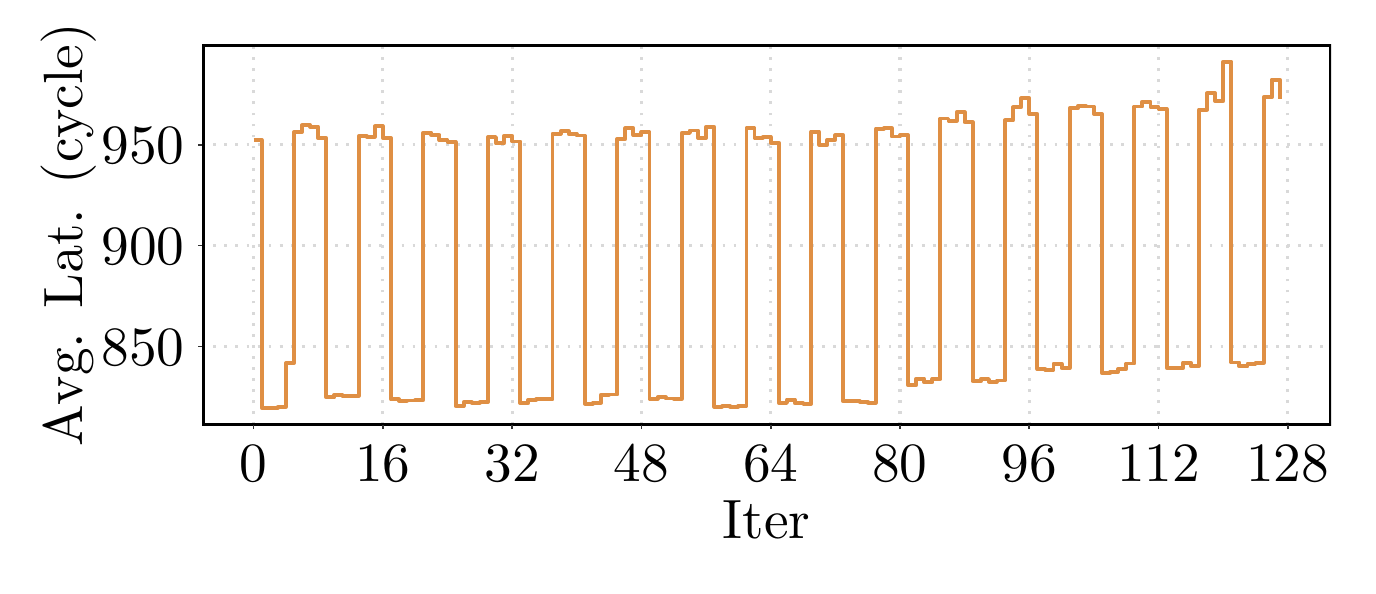
\begin{tikzpicture}[x=1pt,y=1pt]
\definecolor{fillColor}{RGB}{255,255,255}
\path[use as bounding box,fill=fillColor,fill opacity=0.00] (0,0) rectangle (476.98,194.41);
\begin{scope}
\path[clip] (  0.00,  0.00) rectangle (476.98,194.41);
\definecolor{drawColor}{RGB}{255,255,255}
\definecolor{fillColor}{RGB}{255,255,255}

\path[draw=drawColor,line width= 0.6pt,line join=round,line cap=round,fill=fillColor] (  0.00,  0.00) rectangle (476.98,194.41);
\end{scope}
\begin{scope}
\path[clip] ( 63.08, 50.75) rectangle (470.98,188.41);
\definecolor{fillColor}{RGB}{255,255,255}

\path[fill=fillColor] ( 63.08, 50.75) rectangle (470.98,188.41);
\definecolor{drawColor}{gray}{0.85}

\path[draw=drawColor,line width= 1.1pt,dash pattern=on 1pt off 3pt ,line join=round] ( 63.08, 79.23) --
	(470.98, 79.23);

\path[draw=drawColor,line width= 1.1pt,dash pattern=on 1pt off 3pt ,line join=round] ( 63.08,115.67) --
	(470.98,115.67);

\path[draw=drawColor,line width= 1.1pt,dash pattern=on 1pt off 3pt ,line join=round] ( 63.08,152.11) --
	(470.98,152.11);

\path[draw=drawColor,line width= 1.1pt,dash pattern=on 1pt off 3pt ,line join=round] ( 81.62, 50.75) --
	( 81.62,188.41);

\path[draw=drawColor,line width= 1.1pt,dash pattern=on 1pt off 3pt ,line join=round] (128.34, 50.75) --
	(128.34,188.41);

\path[draw=drawColor,line width= 1.1pt,dash pattern=on 1pt off 3pt ,line join=round] (175.05, 50.75) --
	(175.05,188.41);

\path[draw=drawColor,line width= 1.1pt,dash pattern=on 1pt off 3pt ,line join=round] (221.77, 50.75) --
	(221.77,188.41);

\path[draw=drawColor,line width= 1.1pt,dash pattern=on 1pt off 3pt ,line join=round] (268.49, 50.75) --
	(268.49,188.41);

\path[draw=drawColor,line width= 1.1pt,dash pattern=on 1pt off 3pt ,line join=round] (315.21, 50.75) --
	(315.21,188.41);

\path[draw=drawColor,line width= 1.1pt,dash pattern=on 1pt off 3pt ,line join=round] (361.93, 50.75) --
	(361.93,188.41);

\path[draw=drawColor,line width= 1.1pt,dash pattern=on 1pt off 3pt ,line join=round] (408.64, 50.75) --
	(408.64,188.41);

\path[draw=drawColor,line width= 1.1pt,dash pattern=on 1pt off 3pt ,line join=round] (455.36, 50.75) --
	(455.36,188.41);
\definecolor{drawColor}{RGB}{223,143,68}

\path[draw=drawColor,line width= 1.4pt,line join=round] ( 81.62,153.88) --
	( 84.54,153.88) --
	( 84.54, 57.00) --
	( 87.46, 57.00) --
	( 87.46, 57.11) --
	( 90.38, 57.11) --
	( 90.38, 57.42) --
	( 93.30, 57.42) --
	( 93.30, 73.19) --
	( 96.22, 73.19) --
	( 96.22,156.69) --
	( 99.14,156.69) --
	( 99.14,159.14) --
	(102.06,159.14) --
	(102.06,158.67) --
	(104.98,158.67) --
	(104.98,154.40) --
	(107.90,154.40) --
	(107.90, 60.80) --
	(110.82, 60.80) --
	(110.82, 61.74) --
	(113.74, 61.74) --
	(113.74, 61.17) --
	(116.66, 61.17) --
	(116.66, 61.38) --
	(119.58, 61.38) --
	(119.58,155.18) --
	(122.50,155.18) --
	(122.50,155.03) --
	(125.42,155.03) --
	(125.42,158.72) --
	(128.34,158.72) --
	(128.34,154.56) --
	(131.26,154.56) --
	(131.26, 60.08) --
	(134.18, 60.08) --
	(134.18, 59.66) --
	(137.10, 59.66) --
	(137.10, 59.71) --
	(140.02, 59.71) --
	(140.02, 59.76) --
	(142.94, 59.76) --
	(142.94,156.49) --
	(145.86,156.49) --
	(145.86,155.65) --
	(148.78,155.65) --
	(148.78,153.78) --
	(151.70,153.78) --
	(151.70,153.15) --
	(154.62,153.15) --
	(154.62, 57.68) --
	(157.54, 57.68) --
	(157.54, 59.03) --
	(160.45, 59.03) --
	(160.45, 58.88) --
	(163.37, 58.88) --
	(163.37, 59.09) --
	(166.29, 59.09) --
	(166.29,154.87) --
	(169.21,154.87) --
	(169.21,152.58) --
	(172.13,152.58) --
	(172.13,155.34) --
	(175.05,155.34) --
	(175.05,153.26) --
	(177.97,153.26) --
	(177.97, 58.72) --
	(180.89, 58.72) --
	(180.89, 59.92) --
	(183.81, 59.92) --
	(183.81, 60.08) --
	(186.73, 60.08) --
	(186.73, 60.13) --
	(189.65, 60.13) --
	(189.65,156.12) --
	(192.57,156.12) --
	(192.57,156.95) --
	(195.49,156.95) --
	(195.49,155.96) --
	(198.41,155.96) --
	(198.41,155.44) --
	(201.33,155.44) --
	(201.33, 58.57) --
	(204.25, 58.57) --
	(204.25, 58.93) --
	(207.17, 58.93) --
	(207.17, 61.79) --
	(210.09, 61.79) --
	(210.09, 61.85) --
	(213.01, 61.85) --
	(213.01,154.14) --
	(215.93,154.14) --
	(215.93,158.05) --
	(218.85,158.05) --
	(218.85,155.60) --
	(221.77,155.60) --
	(221.77,156.69) --
	(224.69,156.69) --
	(224.69, 60.28) --
	(227.61, 60.28) --
	(227.61, 60.91) --
	(230.53, 60.91) --
	(230.53, 60.39) --
	(233.45, 60.39) --
	(233.45, 60.28) --
	(236.37, 60.28) --
	(236.37,156.38) --
	(239.29,156.38) --
	(239.29,157.27) --
	(242.21,157.27) --
	(242.21,154.61) --
	(245.13,154.61) --
	(245.13,158.57) --
	(248.05,158.57) --
	(248.05, 57.47) --
	(250.97, 57.47) --
	(250.97, 57.63) --
	(253.89, 57.63) --
	(253.89, 57.37) --
	(256.81, 57.37) --
	(256.81, 57.73) --
	(259.73, 57.73) --
	(259.73,158.10) --
	(262.65,158.10) --
	(262.65,154.61) --
	(265.57,154.61) --
	(265.57,154.87) --
	(268.49,154.87) --
	(268.49,152.84) --
	(271.41,152.84) --
	(271.41, 58.83) --
	(274.33, 58.83) --
	(274.33, 60.02) --
	(277.25, 60.02) --
	(277.25, 58.72) --
	(280.17, 58.72) --
	(280.17, 58.46) --
	(283.09, 58.46) --
	(283.09,156.85) --
	(286.01,156.85) --
	(286.01,152.11) --
	(288.93,152.11) --
	(288.93,153.83) --
	(291.85,153.83) --
	(291.85,155.50) --
	(294.77,155.50) --
	(294.77, 59.35) --
	(297.69, 59.35) --
	(297.69, 59.35) --
	(300.61, 59.35) --
	(300.61, 59.24) --
	(303.53, 59.24) --
	(303.53, 58.93) --
	(306.45, 58.93) --
	(306.45,157.89) --
	(309.37,157.89) --
	(309.37,158.05) --
	(312.29,158.05) --
	(312.29,155.08) --
	(315.21,155.08) --
	(315.21,155.55) --
	(318.13,155.55) --
	(318.13, 65.18) --
	(321.05, 65.18) --
	(321.05, 67.57) --
	(323.97, 67.57) --
	(323.97, 66.27) --
	(326.89, 66.27) --
	(326.89, 67.42) --
	(329.81, 67.42) --
	(329.81,161.59) --
	(332.73,161.59) --
	(332.73,160.75) --
	(335.65,160.75) --
	(335.65,163.83) --
	(338.57,163.83) --
	(338.57,160.23) --
	(341.49,160.23) --
	(341.49, 66.64) --
	(344.41, 66.64) --
	(344.41, 67.42) --
	(347.33, 67.42) --
	(347.33, 66.53) --
	(350.25, 66.53) --
	(350.25, 66.90) --
	(353.17, 66.90) --
	(353.17,160.91) --
	(356.09,160.91) --
	(356.09,165.65) --
	(359.01,165.65) --
	(359.01,168.93) --
	(361.93,168.93) --
	(361.93,163.20) --
	(364.85,163.20) --
	(364.85, 71.06) --
	(367.76, 71.06) --
	(367.76, 70.85) --
	(370.68, 70.85) --
	(370.68, 72.99) --
	(373.60, 72.99) --
	(373.60, 71.37) --
	(376.52, 71.37) --
	(376.52,165.23) --
	(379.44,165.23) --
	(379.44,166.06) --
	(382.36,166.06) --
	(382.36,165.91) --
	(385.28,165.91) --
	(385.28,163.20) --
	(388.20,163.20) --
	(388.20, 69.55) --
	(391.12, 69.55) --
	(391.12, 70.02) --
	(394.04, 70.02) --
	(394.04, 71.11) --
	(396.96, 71.11) --
	(396.96, 73.04) --
	(399.88, 73.04) --
	(399.88,165.91) --
	(402.80,165.91) --
	(402.80,167.68) --
	(405.72,167.68) --
	(405.72,165.75) --
	(408.64,165.75) --
	(408.64,165.07) --
	(411.56,165.07) --
	(411.56, 71.53) --
	(414.48, 71.53) --
	(414.48, 71.32) --
	(417.40, 71.32) --
	(417.40, 73.35) --
	(420.32, 73.35) --
	(420.32, 72.15) --
	(423.24, 72.15) --
	(423.24,164.81) --
	(426.16,164.81) --
	(426.16,170.70) --
	(429.08,170.70) --
	(429.08,167.89) --
	(432.00,167.89) --
	(432.00,182.15) --
	(434.92,182.15) --
	(434.92, 73.40) --
	(437.84, 73.40) --
	(437.84, 72.00) --
	(440.76, 72.00) --
	(440.76, 72.93) --
	(443.68, 72.93) --
	(443.68, 73.30) --
	(446.60, 73.30) --
	(446.60,169.24) --
	(449.52,169.24) --
	(449.52,175.59) --
	(452.44,175.59) --
	(452.44,168.77);
\definecolor{drawColor}{RGB}{0,0,0}

\path[draw=drawColor,line width= 1.7pt,line join=round,line cap=round] ( 63.08, 50.75) rectangle (470.98,188.41);
\end{scope}
\begin{scope}
\path[clip] (  0.00,  0.00) rectangle (476.98,194.41);
\definecolor{drawColor}{RGB}{0,0,0}

\node[text=drawColor,anchor=base east,inner sep=0pt, outer sep=0pt, scale=  2.00] at ( 56.66, 72.35) {850};

\node[text=drawColor,anchor=base east,inner sep=0pt, outer sep=0pt, scale=  2.00] at ( 56.66,108.79) {900};

\node[text=drawColor,anchor=base east,inner sep=0pt, outer sep=0pt, scale=  2.00] at ( 56.66,145.23) {950};
\end{scope}
\begin{scope}
\path[clip] (  0.00,  0.00) rectangle (476.98,194.41);
\definecolor{drawColor}{gray}{0.20}

\path[draw=drawColor,line width= 0.6pt,line join=round] ( 61.66, 79.23) --
	( 63.08, 79.23);

\path[draw=drawColor,line width= 0.6pt,line join=round] ( 61.66,115.67) --
	( 63.08,115.67);

\path[draw=drawColor,line width= 0.6pt,line join=round] ( 61.66,152.11) --
	( 63.08,152.11);
\end{scope}
\begin{scope}
\path[clip] (  0.00,  0.00) rectangle (476.98,194.41);
\definecolor{drawColor}{gray}{0.20}

\path[draw=drawColor,line width= 0.6pt,line join=round] ( 81.62, 49.32) --
	( 81.62, 50.75);

\path[draw=drawColor,line width= 0.6pt,line join=round] (128.34, 49.32) --
	(128.34, 50.75);

\path[draw=drawColor,line width= 0.6pt,line join=round] (175.05, 49.32) --
	(175.05, 50.75);

\path[draw=drawColor,line width= 0.6pt,line join=round] (221.77, 49.32) --
	(221.77, 50.75);

\path[draw=drawColor,line width= 0.6pt,line join=round] (268.49, 49.32) --
	(268.49, 50.75);

\path[draw=drawColor,line width= 0.6pt,line join=round] (315.21, 49.32) --
	(315.21, 50.75);

\path[draw=drawColor,line width= 0.6pt,line join=round] (361.93, 49.32) --
	(361.93, 50.75);

\path[draw=drawColor,line width= 0.6pt,line join=round] (408.64, 49.32) --
	(408.64, 50.75);

\path[draw=drawColor,line width= 0.6pt,line join=round] (455.36, 49.32) --
	(455.36, 50.75);
\end{scope}
\begin{scope}
\path[clip] (  0.00,  0.00) rectangle (476.98,194.41);
\definecolor{drawColor}{RGB}{0,0,0}

\node[text=drawColor,anchor=base,inner sep=0pt, outer sep=0pt, scale=  2.00] at ( 81.62, 30.55) {0};

\node[text=drawColor,anchor=base,inner sep=0pt, outer sep=0pt, scale=  2.00] at (128.34, 30.55) {16};

\node[text=drawColor,anchor=base,inner sep=0pt, outer sep=0pt, scale=  2.00] at (175.05, 30.55) {32};

\node[text=drawColor,anchor=base,inner sep=0pt, outer sep=0pt, scale=  2.00] at (221.77, 30.55) {48};

\node[text=drawColor,anchor=base,inner sep=0pt, outer sep=0pt, scale=  2.00] at (268.49, 30.55) {64};

\node[text=drawColor,anchor=base,inner sep=0pt, outer sep=0pt, scale=  2.00] at (315.21, 30.55) {80};

\node[text=drawColor,anchor=base,inner sep=0pt, outer sep=0pt, scale=  2.00] at (361.93, 30.55) {96};

\node[text=drawColor,anchor=base,inner sep=0pt, outer sep=0pt, scale=  2.00] at (408.64, 30.55) {112};

\node[text=drawColor,anchor=base,inner sep=0pt, outer sep=0pt, scale=  2.00] at (455.36, 30.55) {128};
\end{scope}
\begin{scope}
\path[clip] (  0.00,  0.00) rectangle (476.98,194.41);
\definecolor{drawColor}{RGB}{0,0,0}

\node[text=drawColor,anchor=base,inner sep=0pt, outer sep=0pt, scale=  2.00] at (267.03,  9.89) {Iter};
\end{scope}
\begin{scope}
\path[clip] (  0.00,  0.00) rectangle (476.98,194.41);
\definecolor{drawColor}{RGB}{0,0,0}

\node[text=drawColor,rotate= 90.00,anchor=base,inner sep=0pt, outer sep=0pt, scale=  2.00] at ( 19.77,119.58) {Avg. Lat. (cycle)};
\end{scope}
\end{tikzpicture}

\caption{plot/reference/fig9c-covert-vm-signal-receiver.tikz}
\end{figure*}


\begin{figure*}
\centering
% Created by tikzDevice version 0.12.3.1 on 2022-10-11 17:17:09
% !TEX encoding = UTF-8 Unicode
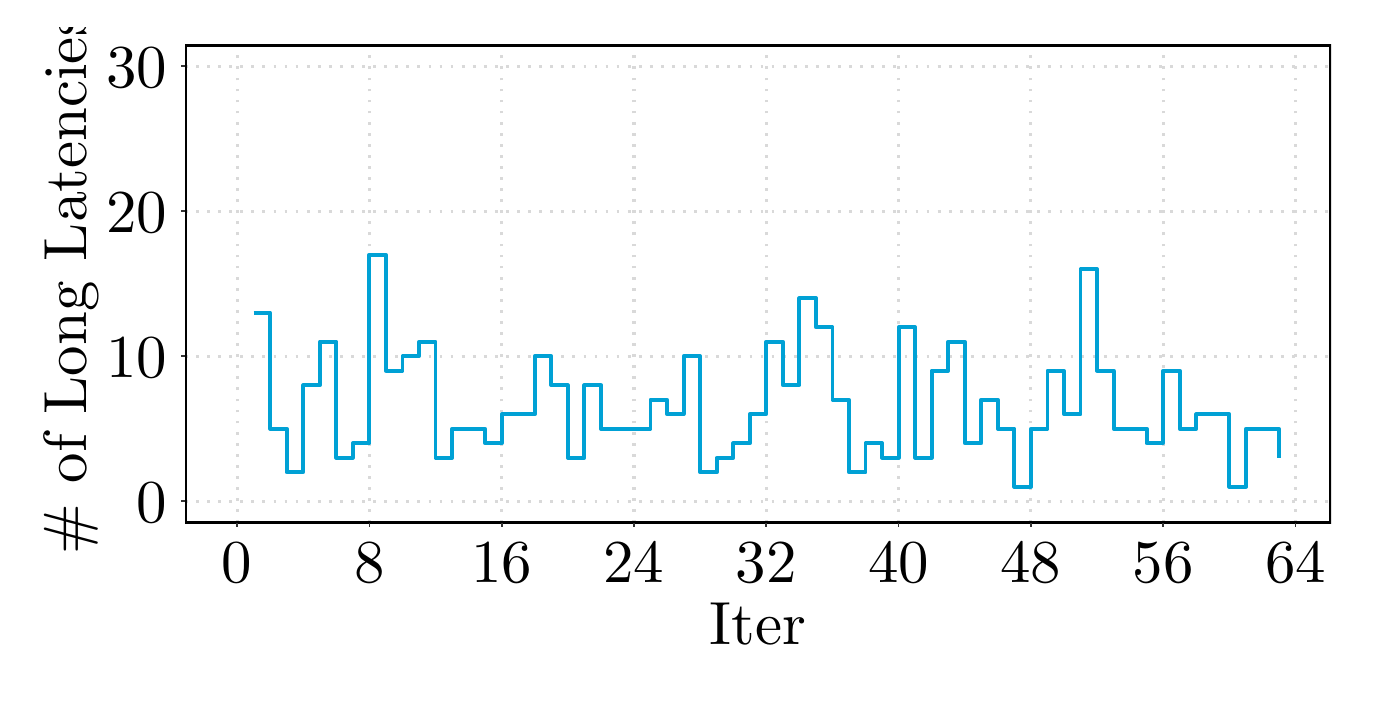
\begin{tikzpicture}[x=1pt,y=1pt]
\definecolor{fillColor}{RGB}{255,255,255}
\path[use as bounding box,fill=fillColor,fill opacity=0.00] (0,0) rectangle (476.98,233.29);
\begin{scope}
\path[clip] (  0.00,  0.00) rectangle (476.98,233.29);
\definecolor{drawColor}{RGB}{255,255,255}
\definecolor{fillColor}{RGB}{255,255,255}

\path[draw=drawColor,line width= 0.6pt,line join=round,line cap=round,fill=fillColor] (  0.00,  0.00) rectangle (476.98,233.29);
\end{scope}
\begin{scope}
\path[clip] ( 56.85, 54.28) rectangle (470.98,227.29);
\definecolor{fillColor}{RGB}{255,255,255}

\path[fill=fillColor] ( 56.85, 54.28) rectangle (470.98,227.29);
\definecolor{drawColor}{gray}{0.85}

\path[draw=drawColor,line width= 1.1pt,dash pattern=on 1pt off 3pt ,line join=round] ( 56.85, 62.14) --
	(470.98, 62.14);

\path[draw=drawColor,line width= 1.1pt,dash pattern=on 1pt off 3pt ,line join=round] ( 56.85,114.57) --
	(470.98,114.57);

\path[draw=drawColor,line width= 1.1pt,dash pattern=on 1pt off 3pt ,line join=round] ( 56.85,167.00) --
	(470.98,167.00);

\path[draw=drawColor,line width= 1.1pt,dash pattern=on 1pt off 3pt ,line join=round] ( 56.85,219.42) --
	(470.98,219.42);

\path[draw=drawColor,line width= 1.1pt,dash pattern=on 1pt off 3pt ,line join=round] ( 75.67, 54.28) --
	( 75.67,227.29);

\path[draw=drawColor,line width= 1.1pt,dash pattern=on 1pt off 3pt ,line join=round] (123.48, 54.28) --
	(123.48,227.29);

\path[draw=drawColor,line width= 1.1pt,dash pattern=on 1pt off 3pt ,line join=round] (171.29, 54.28) --
	(171.29,227.29);

\path[draw=drawColor,line width= 1.1pt,dash pattern=on 1pt off 3pt ,line join=round] (219.09, 54.28) --
	(219.09,227.29);

\path[draw=drawColor,line width= 1.1pt,dash pattern=on 1pt off 3pt ,line join=round] (266.90, 54.28) --
	(266.90,227.29);

\path[draw=drawColor,line width= 1.1pt,dash pattern=on 1pt off 3pt ,line join=round] (314.71, 54.28) --
	(314.71,227.29);

\path[draw=drawColor,line width= 1.1pt,dash pattern=on 1pt off 3pt ,line join=round] (362.52, 54.28) --
	(362.52,227.29);

\path[draw=drawColor,line width= 1.1pt,dash pattern=on 1pt off 3pt ,line join=round] (410.33, 54.28) --
	(410.33,227.29);

\path[draw=drawColor,line width= 1.1pt,dash pattern=on 1pt off 3pt ,line join=round] (458.13, 54.28) --
	(458.13,227.29);
\definecolor{drawColor}{RGB}{0,161,213}

\path[draw=drawColor,line width= 1.4pt,line join=round] ( 81.65,130.30) --
	( 87.62,130.30) --
	( 87.62, 88.36) --
	( 93.60, 88.36) --
	( 93.60, 72.63) --
	( 99.57, 72.63) --
	( 99.57,104.09) --
	(105.55,104.09) --
	(105.55,119.81) --
	(111.53,119.81) --
	(111.53, 77.87) --
	(117.50, 77.87) --
	(117.50, 83.11) --
	(123.48, 83.11) --
	(123.48,151.27) --
	(129.45,151.27) --
	(129.45,109.33) --
	(135.43,109.33) --
	(135.43,114.57) --
	(141.41,114.57) --
	(141.41,119.81) --
	(147.38,119.81) --
	(147.38, 77.87) --
	(153.36, 77.87) --
	(153.36, 88.36) --
	(159.33, 88.36) --
	(159.33, 88.36) --
	(165.31, 88.36) --
	(165.31, 83.11) --
	(171.29, 83.11) --
	(171.29, 93.60) --
	(177.26, 93.60) --
	(177.26, 93.60) --
	(183.24, 93.60) --
	(183.24,114.57) --
	(189.21,114.57) --
	(189.21,104.09) --
	(195.19,104.09) --
	(195.19, 77.87) --
	(201.17, 77.87) --
	(201.17,104.09) --
	(207.14,104.09) --
	(207.14, 88.36) --
	(213.12, 88.36) --
	(213.12, 88.36) --
	(219.09, 88.36) --
	(219.09, 88.36) --
	(225.07, 88.36) --
	(225.07, 98.84) --
	(231.05, 98.84) --
	(231.05, 93.60) --
	(237.02, 93.60) --
	(237.02,114.57) --
	(243.00,114.57) --
	(243.00, 72.63) --
	(248.97, 72.63) --
	(248.97, 77.87) --
	(254.95, 77.87) --
	(254.95, 83.11) --
	(260.93, 83.11) --
	(260.93, 93.60) --
	(266.90, 93.60) --
	(266.90,119.81) --
	(272.88,119.81) --
	(272.88,104.09) --
	(278.85,104.09) --
	(278.85,135.54) --
	(284.83,135.54) --
	(284.83,125.06) --
	(290.81,125.06) --
	(290.81, 98.84) --
	(296.78, 98.84) --
	(296.78, 72.63) --
	(302.76, 72.63) --
	(302.76, 83.11) --
	(308.73, 83.11) --
	(308.73, 77.87) --
	(314.71, 77.87) --
	(314.71,125.06) --
	(320.69,125.06) --
	(320.69, 77.87) --
	(326.66, 77.87) --
	(326.66,109.33) --
	(332.64,109.33) --
	(332.64,119.81) --
	(338.61,119.81) --
	(338.61, 83.11) --
	(344.59, 83.11) --
	(344.59, 98.84) --
	(350.57, 98.84) --
	(350.57, 88.36) --
	(356.54, 88.36) --
	(356.54, 67.39) --
	(362.52, 67.39) --
	(362.52, 88.36) --
	(368.49, 88.36) --
	(368.49,109.33) --
	(374.47,109.33) --
	(374.47, 93.60) --
	(380.45, 93.60) --
	(380.45,146.03) --
	(386.42,146.03) --
	(386.42,109.33) --
	(392.40,109.33) --
	(392.40, 88.36) --
	(398.37, 88.36) --
	(398.37, 88.36) --
	(404.35, 88.36) --
	(404.35, 83.11) --
	(410.33, 83.11) --
	(410.33,109.33) --
	(416.30,109.33) --
	(416.30, 88.36) --
	(422.28, 88.36) --
	(422.28, 93.60) --
	(428.25, 93.60) --
	(428.25, 93.60) --
	(434.23, 93.60) --
	(434.23, 67.39) --
	(440.21, 67.39) --
	(440.21, 88.36) --
	(446.18, 88.36) --
	(446.18, 88.36) --
	(452.16, 88.36) --
	(452.16, 77.87);
\definecolor{drawColor}{RGB}{0,0,0}

\path[draw=drawColor,line width= 1.7pt,line join=round,line cap=round] ( 56.85, 54.28) rectangle (470.98,227.29);
\end{scope}
\begin{scope}
\path[clip] (  0.00,  0.00) rectangle (476.98,233.29);
\definecolor{drawColor}{RGB}{0,0,0}

\node[text=drawColor,anchor=base east,inner sep=0pt, outer sep=0pt, scale=  2.20] at ( 50.42, 54.57) {0};

\node[text=drawColor,anchor=base east,inner sep=0pt, outer sep=0pt, scale=  2.20] at ( 50.42,106.99) {10};

\node[text=drawColor,anchor=base east,inner sep=0pt, outer sep=0pt, scale=  2.20] at ( 50.42,159.42) {20};

\node[text=drawColor,anchor=base east,inner sep=0pt, outer sep=0pt, scale=  2.20] at ( 50.42,211.85) {30};
\end{scope}
\begin{scope}
\path[clip] (  0.00,  0.00) rectangle (476.98,233.29);
\definecolor{drawColor}{gray}{0.20}

\path[draw=drawColor,line width= 0.6pt,line join=round] ( 55.42, 62.14) --
	( 56.85, 62.14);

\path[draw=drawColor,line width= 0.6pt,line join=round] ( 55.42,114.57) --
	( 56.85,114.57);

\path[draw=drawColor,line width= 0.6pt,line join=round] ( 55.42,167.00) --
	( 56.85,167.00);

\path[draw=drawColor,line width= 0.6pt,line join=round] ( 55.42,219.42) --
	( 56.85,219.42);
\end{scope}
\begin{scope}
\path[clip] (  0.00,  0.00) rectangle (476.98,233.29);
\definecolor{drawColor}{gray}{0.20}

\path[draw=drawColor,line width= 0.6pt,line join=round] ( 75.67, 52.86) --
	( 75.67, 54.28);

\path[draw=drawColor,line width= 0.6pt,line join=round] (123.48, 52.86) --
	(123.48, 54.28);

\path[draw=drawColor,line width= 0.6pt,line join=round] (171.29, 52.86) --
	(171.29, 54.28);

\path[draw=drawColor,line width= 0.6pt,line join=round] (219.09, 52.86) --
	(219.09, 54.28);

\path[draw=drawColor,line width= 0.6pt,line join=round] (266.90, 52.86) --
	(266.90, 54.28);

\path[draw=drawColor,line width= 0.6pt,line join=round] (314.71, 52.86) --
	(314.71, 54.28);

\path[draw=drawColor,line width= 0.6pt,line join=round] (362.52, 52.86) --
	(362.52, 54.28);

\path[draw=drawColor,line width= 0.6pt,line join=round] (410.33, 52.86) --
	(410.33, 54.28);

\path[draw=drawColor,line width= 0.6pt,line join=round] (458.13, 52.86) --
	(458.13, 54.28);
\end{scope}
\begin{scope}
\path[clip] (  0.00,  0.00) rectangle (476.98,233.29);
\definecolor{drawColor}{RGB}{0,0,0}

\node[text=drawColor,anchor=base,inner sep=0pt, outer sep=0pt, scale=  2.20] at ( 75.67, 32.71) {0};

\node[text=drawColor,anchor=base,inner sep=0pt, outer sep=0pt, scale=  2.20] at (123.48, 32.71) {8};

\node[text=drawColor,anchor=base,inner sep=0pt, outer sep=0pt, scale=  2.20] at (171.29, 32.71) {16};

\node[text=drawColor,anchor=base,inner sep=0pt, outer sep=0pt, scale=  2.20] at (219.09, 32.71) {24};

\node[text=drawColor,anchor=base,inner sep=0pt, outer sep=0pt, scale=  2.20] at (266.90, 32.71) {32};

\node[text=drawColor,anchor=base,inner sep=0pt, outer sep=0pt, scale=  2.20] at (314.71, 32.71) {40};

\node[text=drawColor,anchor=base,inner sep=0pt, outer sep=0pt, scale=  2.20] at (362.52, 32.71) {48};

\node[text=drawColor,anchor=base,inner sep=0pt, outer sep=0pt, scale=  2.20] at (410.33, 32.71) {56};

\node[text=drawColor,anchor=base,inner sep=0pt, outer sep=0pt, scale=  2.20] at (458.13, 32.71) {64};
\end{scope}
\begin{scope}
\path[clip] (  0.00,  0.00) rectangle (476.98,233.29);
\definecolor{drawColor}{RGB}{0,0,0}

\node[text=drawColor,anchor=base,inner sep=0pt, outer sep=0pt, scale=  2.20] at (263.91, 10.28) {Iter};
\end{scope}
\begin{scope}
\path[clip] (  0.00,  0.00) rectangle (476.98,233.29);
\definecolor{drawColor}{RGB}{0,0,0}

\node[text=drawColor,rotate= 90.00,anchor=base,inner sep=0pt, outer sep=0pt, scale=  2.20] at ( 21.15,140.78) {\# of Long Latencies};
\end{scope}
\end{tikzpicture}

\caption{plot/reference/fig10a-covert-inode-pmem.tikz}
\end{figure*}


\begin{figure*}
\centering
% Created by tikzDevice version 0.12.3.1 on 2022-10-11 17:17:09
% !TEX encoding = UTF-8 Unicode
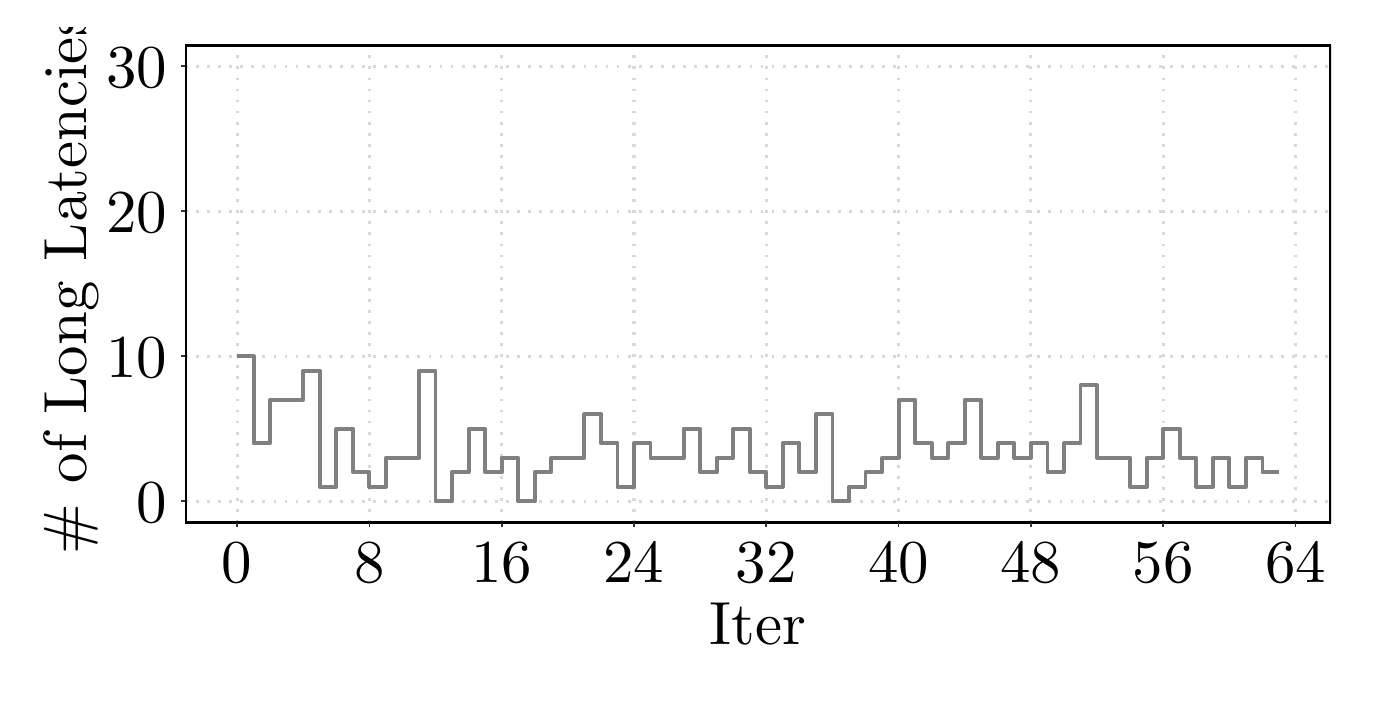
\begin{tikzpicture}[x=1pt,y=1pt]
\definecolor{fillColor}{RGB}{255,255,255}
\path[use as bounding box,fill=fillColor,fill opacity=0.00] (0,0) rectangle (476.98,233.29);
\begin{scope}
\path[clip] (  0.00,  0.00) rectangle (476.98,233.29);
\definecolor{drawColor}{RGB}{255,255,255}
\definecolor{fillColor}{RGB}{255,255,255}

\path[draw=drawColor,line width= 0.6pt,line join=round,line cap=round,fill=fillColor] (  0.00,  0.00) rectangle (476.98,233.29);
\end{scope}
\begin{scope}
\path[clip] ( 56.85, 54.28) rectangle (470.98,227.29);
\definecolor{fillColor}{RGB}{255,255,255}

\path[fill=fillColor] ( 56.85, 54.28) rectangle (470.98,227.29);
\definecolor{drawColor}{gray}{0.85}

\path[draw=drawColor,line width= 1.1pt,dash pattern=on 1pt off 3pt ,line join=round] ( 56.85, 62.14) --
	(470.98, 62.14);

\path[draw=drawColor,line width= 1.1pt,dash pattern=on 1pt off 3pt ,line join=round] ( 56.85,114.57) --
	(470.98,114.57);

\path[draw=drawColor,line width= 1.1pt,dash pattern=on 1pt off 3pt ,line join=round] ( 56.85,167.00) --
	(470.98,167.00);

\path[draw=drawColor,line width= 1.1pt,dash pattern=on 1pt off 3pt ,line join=round] ( 56.85,219.42) --
	(470.98,219.42);

\path[draw=drawColor,line width= 1.1pt,dash pattern=on 1pt off 3pt ,line join=round] ( 75.67, 54.28) --
	( 75.67,227.29);

\path[draw=drawColor,line width= 1.1pt,dash pattern=on 1pt off 3pt ,line join=round] (123.48, 54.28) --
	(123.48,227.29);

\path[draw=drawColor,line width= 1.1pt,dash pattern=on 1pt off 3pt ,line join=round] (171.29, 54.28) --
	(171.29,227.29);

\path[draw=drawColor,line width= 1.1pt,dash pattern=on 1pt off 3pt ,line join=round] (219.09, 54.28) --
	(219.09,227.29);

\path[draw=drawColor,line width= 1.1pt,dash pattern=on 1pt off 3pt ,line join=round] (266.90, 54.28) --
	(266.90,227.29);

\path[draw=drawColor,line width= 1.1pt,dash pattern=on 1pt off 3pt ,line join=round] (314.71, 54.28) --
	(314.71,227.29);

\path[draw=drawColor,line width= 1.1pt,dash pattern=on 1pt off 3pt ,line join=round] (362.52, 54.28) --
	(362.52,227.29);

\path[draw=drawColor,line width= 1.1pt,dash pattern=on 1pt off 3pt ,line join=round] (410.33, 54.28) --
	(410.33,227.29);

\path[draw=drawColor,line width= 1.1pt,dash pattern=on 1pt off 3pt ,line join=round] (458.13, 54.28) --
	(458.13,227.29);
\definecolor{drawColor}{gray}{0.50}

\path[draw=drawColor,line width= 1.4pt,line join=round] ( 75.67,114.57) --
	( 81.65,114.57) --
	( 81.65, 83.11) --
	( 87.62, 83.11) --
	( 87.62, 98.84) --
	( 93.60, 98.84) --
	( 93.60, 98.84) --
	( 99.57, 98.84) --
	( 99.57,109.33) --
	(105.55,109.33) --
	(105.55, 67.39) --
	(111.53, 67.39) --
	(111.53, 88.36) --
	(117.50, 88.36) --
	(117.50, 72.63) --
	(123.48, 72.63) --
	(123.48, 67.39) --
	(129.45, 67.39) --
	(129.45, 77.87) --
	(135.43, 77.87) --
	(135.43, 77.87) --
	(141.41, 77.87) --
	(141.41,109.33) --
	(147.38,109.33) --
	(147.38, 62.14) --
	(153.36, 62.14) --
	(153.36, 72.63) --
	(159.33, 72.63) --
	(159.33, 88.36) --
	(165.31, 88.36) --
	(165.31, 72.63) --
	(171.29, 72.63) --
	(171.29, 77.87) --
	(177.26, 77.87) --
	(177.26, 62.14) --
	(183.24, 62.14) --
	(183.24, 72.63) --
	(189.21, 72.63) --
	(189.21, 77.87) --
	(195.19, 77.87) --
	(195.19, 77.87) --
	(201.17, 77.87) --
	(201.17, 93.60) --
	(207.14, 93.60) --
	(207.14, 83.11) --
	(213.12, 83.11) --
	(213.12, 67.39) --
	(219.09, 67.39) --
	(219.09, 83.11) --
	(225.07, 83.11) --
	(225.07, 77.87) --
	(231.05, 77.87) --
	(231.05, 77.87) --
	(237.02, 77.87) --
	(237.02, 88.36) --
	(243.00, 88.36) --
	(243.00, 72.63) --
	(248.97, 72.63) --
	(248.97, 77.87) --
	(254.95, 77.87) --
	(254.95, 88.36) --
	(260.93, 88.36) --
	(260.93, 72.63) --
	(266.90, 72.63) --
	(266.90, 67.39) --
	(272.88, 67.39) --
	(272.88, 83.11) --
	(278.85, 83.11) --
	(278.85, 72.63) --
	(284.83, 72.63) --
	(284.83, 93.60) --
	(290.81, 93.60) --
	(290.81, 62.14) --
	(296.78, 62.14) --
	(296.78, 67.39) --
	(302.76, 67.39) --
	(302.76, 72.63) --
	(308.73, 72.63) --
	(308.73, 77.87) --
	(314.71, 77.87) --
	(314.71, 98.84) --
	(320.69, 98.84) --
	(320.69, 83.11) --
	(326.66, 83.11) --
	(326.66, 77.87) --
	(332.64, 77.87) --
	(332.64, 83.11) --
	(338.61, 83.11) --
	(338.61, 98.84) --
	(344.59, 98.84) --
	(344.59, 77.87) --
	(350.57, 77.87) --
	(350.57, 83.11) --
	(356.54, 83.11) --
	(356.54, 77.87) --
	(362.52, 77.87) --
	(362.52, 83.11) --
	(368.49, 83.11) --
	(368.49, 72.63) --
	(374.47, 72.63) --
	(374.47, 83.11) --
	(380.45, 83.11) --
	(380.45,104.09) --
	(386.42,104.09) --
	(386.42, 77.87) --
	(392.40, 77.87) --
	(392.40, 77.87) --
	(398.37, 77.87) --
	(398.37, 67.39) --
	(404.35, 67.39) --
	(404.35, 77.87) --
	(410.33, 77.87) --
	(410.33, 88.36) --
	(416.30, 88.36) --
	(416.30, 77.87) --
	(422.28, 77.87) --
	(422.28, 67.39) --
	(428.25, 67.39) --
	(428.25, 77.87) --
	(434.23, 77.87) --
	(434.23, 67.39) --
	(440.21, 67.39) --
	(440.21, 77.87) --
	(446.18, 77.87) --
	(446.18, 72.63) --
	(452.16, 72.63) --
	(452.16, 72.63);
\definecolor{drawColor}{RGB}{0,0,0}

\path[draw=drawColor,line width= 1.7pt,line join=round,line cap=round] ( 56.85, 54.28) rectangle (470.98,227.29);
\end{scope}
\begin{scope}
\path[clip] (  0.00,  0.00) rectangle (476.98,233.29);
\definecolor{drawColor}{RGB}{0,0,0}

\node[text=drawColor,anchor=base east,inner sep=0pt, outer sep=0pt, scale=  2.20] at ( 50.42, 54.57) {0};

\node[text=drawColor,anchor=base east,inner sep=0pt, outer sep=0pt, scale=  2.20] at ( 50.42,106.99) {10};

\node[text=drawColor,anchor=base east,inner sep=0pt, outer sep=0pt, scale=  2.20] at ( 50.42,159.42) {20};

\node[text=drawColor,anchor=base east,inner sep=0pt, outer sep=0pt, scale=  2.20] at ( 50.42,211.85) {30};
\end{scope}
\begin{scope}
\path[clip] (  0.00,  0.00) rectangle (476.98,233.29);
\definecolor{drawColor}{gray}{0.20}

\path[draw=drawColor,line width= 0.6pt,line join=round] ( 55.42, 62.14) --
	( 56.85, 62.14);

\path[draw=drawColor,line width= 0.6pt,line join=round] ( 55.42,114.57) --
	( 56.85,114.57);

\path[draw=drawColor,line width= 0.6pt,line join=round] ( 55.42,167.00) --
	( 56.85,167.00);

\path[draw=drawColor,line width= 0.6pt,line join=round] ( 55.42,219.42) --
	( 56.85,219.42);
\end{scope}
\begin{scope}
\path[clip] (  0.00,  0.00) rectangle (476.98,233.29);
\definecolor{drawColor}{gray}{0.20}

\path[draw=drawColor,line width= 0.6pt,line join=round] ( 75.67, 52.86) --
	( 75.67, 54.28);

\path[draw=drawColor,line width= 0.6pt,line join=round] (123.48, 52.86) --
	(123.48, 54.28);

\path[draw=drawColor,line width= 0.6pt,line join=round] (171.29, 52.86) --
	(171.29, 54.28);

\path[draw=drawColor,line width= 0.6pt,line join=round] (219.09, 52.86) --
	(219.09, 54.28);

\path[draw=drawColor,line width= 0.6pt,line join=round] (266.90, 52.86) --
	(266.90, 54.28);

\path[draw=drawColor,line width= 0.6pt,line join=round] (314.71, 52.86) --
	(314.71, 54.28);

\path[draw=drawColor,line width= 0.6pt,line join=round] (362.52, 52.86) --
	(362.52, 54.28);

\path[draw=drawColor,line width= 0.6pt,line join=round] (410.33, 52.86) --
	(410.33, 54.28);

\path[draw=drawColor,line width= 0.6pt,line join=round] (458.13, 52.86) --
	(458.13, 54.28);
\end{scope}
\begin{scope}
\path[clip] (  0.00,  0.00) rectangle (476.98,233.29);
\definecolor{drawColor}{RGB}{0,0,0}

\node[text=drawColor,anchor=base,inner sep=0pt, outer sep=0pt, scale=  2.20] at ( 75.67, 32.71) {0};

\node[text=drawColor,anchor=base,inner sep=0pt, outer sep=0pt, scale=  2.20] at (123.48, 32.71) {8};

\node[text=drawColor,anchor=base,inner sep=0pt, outer sep=0pt, scale=  2.20] at (171.29, 32.71) {16};

\node[text=drawColor,anchor=base,inner sep=0pt, outer sep=0pt, scale=  2.20] at (219.09, 32.71) {24};

\node[text=drawColor,anchor=base,inner sep=0pt, outer sep=0pt, scale=  2.20] at (266.90, 32.71) {32};

\node[text=drawColor,anchor=base,inner sep=0pt, outer sep=0pt, scale=  2.20] at (314.71, 32.71) {40};

\node[text=drawColor,anchor=base,inner sep=0pt, outer sep=0pt, scale=  2.20] at (362.52, 32.71) {48};

\node[text=drawColor,anchor=base,inner sep=0pt, outer sep=0pt, scale=  2.20] at (410.33, 32.71) {56};

\node[text=drawColor,anchor=base,inner sep=0pt, outer sep=0pt, scale=  2.20] at (458.13, 32.71) {64};
\end{scope}
\begin{scope}
\path[clip] (  0.00,  0.00) rectangle (476.98,233.29);
\definecolor{drawColor}{RGB}{0,0,0}

\node[text=drawColor,anchor=base,inner sep=0pt, outer sep=0pt, scale=  2.20] at (263.91, 10.28) {Iter};
\end{scope}
\begin{scope}
\path[clip] (  0.00,  0.00) rectangle (476.98,233.29);
\definecolor{drawColor}{RGB}{0,0,0}

\node[text=drawColor,rotate= 90.00,anchor=base,inner sep=0pt, outer sep=0pt, scale=  2.20] at ( 21.15,140.78) {\# of Long Latencies};
\end{scope}
\end{tikzpicture}

\caption{plot/reference/fig10b-covert-inode-dram.tikz}
\end{figure*}


\begin{figure*}
\centering
% Created by tikzDevice version 0.12.3.1 on 2022-10-13 03:32:19
% !TEX encoding = UTF-8 Unicode
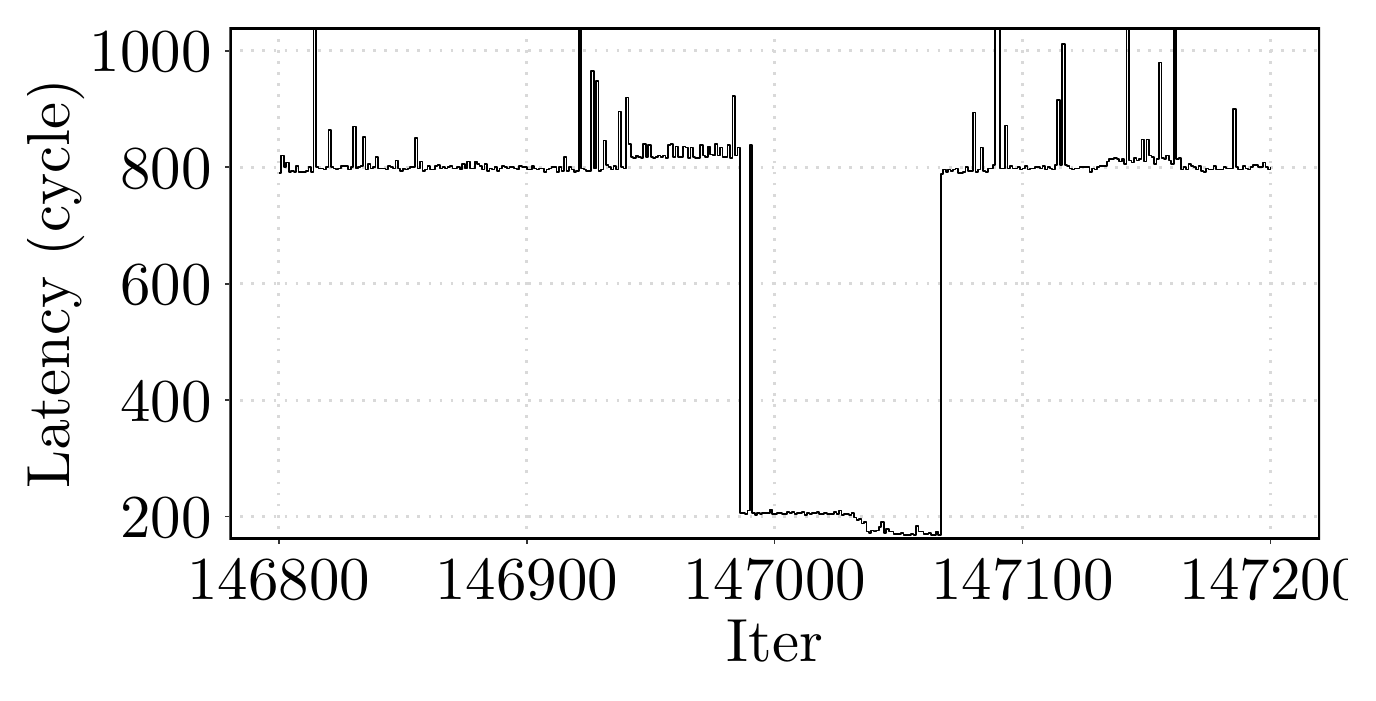
\begin{tikzpicture}[x=1pt,y=1pt]
\definecolor{fillColor}{RGB}{255,255,255}
\path[use as bounding box,fill=fillColor,fill opacity=0.00] (0,0) rectangle (476.98,233.29);
\begin{scope}
\path[clip] (  0.00,  0.00) rectangle (476.98,233.29);
\definecolor{drawColor}{RGB}{255,255,255}
\definecolor{fillColor}{RGB}{255,255,255}

\path[draw=drawColor,line width= 0.6pt,line join=round,line cap=round,fill=fillColor] (  0.00,  0.00) rectangle (476.98,233.29);
\end{scope}
\begin{scope}
\path[clip] ( 72.84, 48.28) rectangle (466.98,233.29);
\definecolor{fillColor}{RGB}{255,255,255}

\path[fill=fillColor] ( 72.84, 48.28) rectangle (466.98,233.29);
\definecolor{drawColor}{gray}{0.85}

\path[draw=drawColor,line width= 1.1pt,dash pattern=on 1pt off 3pt ,line join=round] ( 72.84, 56.69) --
	(466.98, 56.69);

\path[draw=drawColor,line width= 1.1pt,dash pattern=on 1pt off 3pt ,line join=round] ( 72.84, 98.74) --
	(466.98, 98.74);

\path[draw=drawColor,line width= 1.1pt,dash pattern=on 1pt off 3pt ,line join=round] ( 72.84,140.78) --
	(466.98,140.78);

\path[draw=drawColor,line width= 1.1pt,dash pattern=on 1pt off 3pt ,line join=round] ( 72.84,182.83) --
	(466.98,182.83);

\path[draw=drawColor,line width= 1.1pt,dash pattern=on 1pt off 3pt ,line join=round] ( 72.84,224.88) --
	(466.98,224.88);

\path[draw=drawColor,line width= 1.1pt,dash pattern=on 1pt off 3pt ,line join=round] ( 90.76, 48.28) --
	( 90.76,233.29);

\path[draw=drawColor,line width= 1.1pt,dash pattern=on 1pt off 3pt ,line join=round] (180.33, 48.28) --
	(180.33,233.29);

\path[draw=drawColor,line width= 1.1pt,dash pattern=on 1pt off 3pt ,line join=round] (269.91, 48.28) --
	(269.91,233.29);

\path[draw=drawColor,line width= 1.1pt,dash pattern=on 1pt off 3pt ,line join=round] (359.49, 48.28) --
	(359.49,233.29);

\path[draw=drawColor,line width= 1.1pt,dash pattern=on 1pt off 3pt ,line join=round] (449.07, 48.28) --
	(449.07,233.29);
\definecolor{drawColor}{RGB}{0,0,0}

\path[draw=drawColor,line width= 0.6pt,line join=round] ( 90.76,180.73) --
	( 91.65,180.73) --
	( 91.65,187.04) --
	( 92.55,187.04) --
	( 92.55,182.83) --
	( 93.44,182.83) --
	( 93.44,184.51) --
	( 94.34,184.51) --
	( 94.34,181.15) --
	( 95.23,181.15) --
	( 95.23,181.57) --
	( 96.13,181.57) --
	( 96.13,181.15) --
	( 97.03,181.15) --
	( 97.03,183.25) --
	( 97.92,183.25) --
	( 97.92,181.15) --
	( 98.82,181.15) --
	( 98.82,181.15) --
	( 99.71,181.15) --
	( 99.71,181.15) --
	(100.61,181.15) --
	(100.61,181.57) --
	(101.51,181.57) --
	(101.51,182.83) --
	(102.40,182.83) --
	(102.40,181.15) --
	(103.30,181.15) --
	(103.30,235.81) --
	(104.19,235.81) --
	(104.19,182.83) --
	(105.09,182.83) --
	(105.09,182.41) --
	(105.98,182.41) --
	(105.98,182.41) --
	(106.88,182.41) --
	(106.88,181.99) --
	(107.78,181.99) --
	(107.78,182.83) --
	(108.67,182.83) --
	(108.67,196.29) --
	(109.57,196.29) --
	(109.57,182.83) --
	(110.46,182.83) --
	(110.46,182.41) --
	(111.36,182.41) --
	(111.36,181.99) --
	(112.25,181.99) --
	(112.25,182.41) --
	(113.15,182.41) --
	(113.15,183.25) --
	(114.05,183.25) --
	(114.05,183.25) --
	(114.94,183.25) --
	(114.94,183.25) --
	(115.84,183.25) --
	(115.84,181.99) --
	(116.73,181.99) --
	(116.73,182.83) --
	(117.63,182.83) --
	(117.63,197.55) --
	(118.52,197.55) --
	(118.52,182.41) --
	(119.42,182.41) --
	(119.42,182.83) --
	(120.32,182.83) --
	(120.32,183.25) --
	(121.21,183.25) --
	(121.21,193.76) --
	(122.11,193.76) --
	(122.11,181.99) --
	(123.00,181.99) --
	(123.00,184.09) --
	(123.90,184.09) --
	(123.90,182.41) --
	(124.80,182.41) --
	(124.80,182.83) --
	(125.69,182.83) --
	(125.69,186.62) --
	(126.59,186.62) --
	(126.59,182.41) --
	(127.48,182.41) --
	(127.48,182.41) --
	(128.38,182.41) --
	(128.38,182.41) --
	(129.27,182.41) --
	(129.27,181.99) --
	(130.17,181.99) --
	(130.17,183.25) --
	(131.07,183.25) --
	(131.07,182.83) --
	(131.96,182.83) --
	(131.96,182.41) --
	(132.86,182.41) --
	(132.86,185.35) --
	(133.75,185.35) --
	(133.75,182.41) --
	(134.65,182.41) --
	(134.65,181.57) --
	(135.54,181.57) --
	(135.54,182.41) --
	(136.44,182.41) --
	(136.44,181.99) --
	(137.34,181.99) --
	(137.34,182.41) --
	(138.23,182.41) --
	(138.23,182.83) --
	(139.13,182.83) --
	(139.13,182.83) --
	(140.02,182.83) --
	(140.02,193.34) --
	(140.92,193.34) --
	(140.92,182.41) --
	(141.82,182.41) --
	(141.82,184.93) --
	(142.71,184.93) --
	(142.71,181.57) --
	(143.61,181.57) --
	(143.61,181.99) --
	(144.50,181.99) --
	(144.50,183.25) --
	(145.40,183.25) --
	(145.40,181.99) --
	(146.29,181.99) --
	(146.29,181.99) --
	(147.19,181.99) --
	(147.19,183.25) --
	(148.09,183.25) --
	(148.09,183.67) --
	(148.98,183.67) --
	(148.98,182.41) --
	(149.88,182.41) --
	(149.88,182.83) --
	(150.77,182.83) --
	(150.77,182.41) --
	(151.67,182.41) --
	(151.67,182.83) --
	(152.56,182.83) --
	(152.56,183.25) --
	(153.46,183.25) --
	(153.46,182.41) --
	(154.36,182.41) --
	(154.36,182.41) --
	(155.25,182.41) --
	(155.25,182.83) --
	(156.15,182.83) --
	(156.15,181.99) --
	(157.04,181.99) --
	(157.04,184.09) --
	(157.94,184.09) --
	(157.94,182.41) --
	(158.83,182.41) --
	(158.83,184.93) --
	(159.73,184.93) --
	(159.73,182.41) --
	(160.63,182.41) --
	(160.63,182.41) --
	(161.52,182.41) --
	(161.52,184.93) --
	(162.42,184.93) --
	(162.42,184.09) --
	(163.31,184.09) --
	(163.31,183.25) --
	(164.21,183.25) --
	(164.21,181.99) --
	(165.11,181.99) --
	(165.11,184.09) --
	(166.00,184.09) --
	(166.00,181.57) --
	(166.90,181.57) --
	(166.90,182.41) --
	(167.79,182.41) --
	(167.79,181.99) --
	(168.69,181.99) --
	(168.69,182.83) --
	(169.58,182.83) --
	(169.58,181.57) --
	(170.48,181.57) --
	(170.48,182.41) --
	(171.38,182.41) --
	(171.38,183.25) --
	(172.27,183.25) --
	(172.27,182.83) --
	(173.17,182.83) --
	(173.17,182.41) --
	(174.06,182.41) --
	(174.06,182.83) --
	(174.96,182.83) --
	(174.96,182.83) --
	(175.85,182.83) --
	(175.85,182.41) --
	(176.75,182.41) --
	(176.75,181.99) --
	(177.65,181.99) --
	(177.65,183.25) --
	(178.54,183.25) --
	(178.54,182.83) --
	(179.44,182.83) --
	(179.44,182.83) --
	(180.33,182.83) --
	(180.33,181.99) --
	(181.23,181.99) --
	(181.23,181.99) --
	(182.13,181.99) --
	(182.13,183.25) --
	(183.02,183.25) --
	(183.02,182.41) --
	(183.92,182.41) --
	(183.92,181.99) --
	(184.81,181.99) --
	(184.81,182.41) --
	(185.71,182.41) --
	(185.71,182.41) --
	(186.60,182.41) --
	(186.60,181.15) --
	(187.50,181.15) --
	(187.50,181.99) --
	(188.40,181.99) --
	(188.40,182.41) --
	(189.29,182.41) --
	(189.29,182.83) --
	(190.19,182.83) --
	(190.19,182.83) --
	(191.08,182.83) --
	(191.08,181.15) --
	(191.98,181.15) --
	(191.98,182.83) --
	(192.87,182.83) --
	(192.87,181.57) --
	(193.77,181.57) --
	(193.77,186.62) --
	(194.67,186.62) --
	(194.67,181.57) --
	(195.56,181.57) --
	(195.56,182.83) --
	(196.46,182.83) --
	(196.46,181.99) --
	(197.35,181.99) --
	(197.35,181.15) --
	(198.25,181.15) --
	(198.25,181.57) --
	(199.14,181.57) --
	(199.14,235.81) --
	(200.04,235.81) --
	(200.04,182.41) --
	(200.94,182.41) --
	(200.94,181.99) --
	(201.83,181.99) --
	(201.83,181.57) --
	(202.73,181.57) --
	(202.73,181.57) --
	(203.62,181.57) --
	(203.62,217.73) --
	(204.52,217.73) --
	(204.52,182.41) --
	(205.42,182.41) --
	(205.42,213.95) --
	(206.31,213.95) --
	(206.31,181.57) --
	(207.21,181.57) --
	(207.21,181.99) --
	(208.10,181.99) --
	(208.10,192.50) --
	(209.00,192.50) --
	(209.00,183.67) --
	(209.89,183.67) --
	(209.89,182.83) --
	(210.79,182.83) --
	(210.79,181.99) --
	(211.69,181.99) --
	(211.69,183.25) --
	(212.58,183.25) --
	(212.58,181.99) --
	(213.48,181.99) --
	(213.48,203.01) --
	(214.37,203.01) --
	(214.37,182.83) --
	(215.27,182.83) --
	(215.27,182.41) --
	(216.16,182.41) --
	(216.16,208.06) --
	(217.06,208.06) --
	(217.06,191.24) --
	(217.96,191.24) --
	(217.96,186.62) --
	(218.85,186.62) --
	(218.85,186.19) --
	(219.75,186.19) --
	(219.75,187.04) --
	(220.64,187.04) --
	(220.64,186.62) --
	(221.54,186.62) --
	(221.54,186.19) --
	(222.44,186.19) --
	(222.44,191.24) --
	(223.33,191.24) --
	(223.33,186.62) --
	(224.23,186.62) --
	(224.23,190.82) --
	(225.12,190.82) --
	(225.12,186.62) --
	(226.02,186.62) --
	(226.02,186.19) --
	(226.91,186.19) --
	(226.91,186.62) --
	(227.81,186.62) --
	(227.81,187.04) --
	(228.71,187.04) --
	(228.71,186.62) --
	(229.60,186.62) --
	(229.60,187.04) --
	(230.50,187.04) --
	(230.50,186.19) --
	(231.39,186.19) --
	(231.39,190.82) --
	(232.29,190.82) --
	(232.29,191.24) --
	(233.18,191.24) --
	(233.18,186.62) --
	(234.08,186.62) --
	(234.08,190.40) --
	(234.98,190.40) --
	(234.98,186.62) --
	(235.87,186.62) --
	(235.87,186.62) --
	(236.77,186.62) --
	(236.77,190.40) --
	(237.66,190.40) --
	(237.66,189.98) --
	(238.56,189.98) --
	(238.56,186.19) --
	(239.45,186.19) --
	(239.45,189.98) --
	(240.35,189.98) --
	(240.35,186.62) --
	(241.25,186.62) --
	(241.25,186.19) --
	(242.14,186.19) --
	(242.14,186.19) --
	(243.04,186.19) --
	(243.04,190.82) --
	(243.93,190.82) --
	(243.93,187.04) --
	(244.83,187.04) --
	(244.83,186.62) --
	(245.73,186.62) --
	(245.73,190.40) --
	(246.62,190.40) --
	(246.62,187.46) --
	(247.52,187.46) --
	(247.52,187.04) --
	(248.41,187.04) --
	(248.41,191.24) --
	(249.31,191.24) --
	(249.31,187.04) --
	(250.20,187.04) --
	(250.20,189.98) --
	(251.10,189.98) --
	(251.10,186.62) --
	(252.00,186.62) --
	(252.00,186.62) --
	(252.89,186.62) --
	(252.89,190.82) --
	(253.79,190.82) --
	(253.79,186.19) --
	(254.68,186.19) --
	(254.68,208.48) --
	(255.58,208.48) --
	(255.58,187.04) --
	(256.47,187.04) --
	(256.47,189.98) --
	(257.37,189.98) --
	(257.37, 57.95) --
	(258.27, 57.95) --
	(258.27, 57.95) --
	(259.16, 57.95) --
	(259.16, 57.53) --
	(260.06, 57.53) --
	(260.06, 58.79) --
	(260.95, 58.79) --
	(260.95,190.82) --
	(261.85,190.82) --
	(261.85, 57.95) --
	(262.74, 57.95) --
	(262.74, 57.11) --
	(263.64, 57.11) --
	(263.64, 57.95) --
	(264.54, 57.95) --
	(264.54, 57.53) --
	(265.43, 57.53) --
	(265.43, 57.95) --
	(266.33, 57.95) --
	(266.33, 57.95) --
	(267.22, 57.95) --
	(267.22, 57.95) --
	(268.12, 57.95) --
	(268.12, 59.21) --
	(269.02, 59.21) --
	(269.02, 57.53) --
	(269.91, 57.53) --
	(269.91, 57.53) --
	(270.81, 57.53) --
	(270.81, 57.95) --
	(271.70, 57.95) --
	(271.70, 57.95) --
	(272.60, 57.95) --
	(272.60, 57.53) --
	(273.49, 57.53) --
	(273.49, 57.53) --
	(274.39, 57.53) --
	(274.39, 58.37) --
	(275.29, 58.37) --
	(275.29, 57.95) --
	(276.18, 57.95) --
	(276.18, 58.37) --
	(277.08, 58.37) --
	(277.08, 57.53) --
	(277.97, 57.53) --
	(277.97, 57.95) --
	(278.87, 57.95) --
	(278.87, 57.95) --
	(279.76, 57.95) --
	(279.76, 58.37) --
	(280.66, 58.37) --
	(280.66, 57.11) --
	(281.56, 57.11) --
	(281.56, 57.95) --
	(282.45, 57.95) --
	(282.45, 57.53) --
	(283.35, 57.53) --
	(283.35, 57.95) --
	(284.24, 57.95) --
	(284.24, 57.95) --
	(285.14, 57.95) --
	(285.14, 58.37) --
	(286.04, 58.37) --
	(286.04, 57.53) --
	(286.93, 57.53) --
	(286.93, 57.53) --
	(287.83, 57.53) --
	(287.83, 57.95) --
	(288.72, 57.95) --
	(288.72, 57.53) --
	(289.62, 57.53) --
	(289.62, 57.53) --
	(290.51, 57.53) --
	(290.51, 57.53) --
	(291.41, 57.53) --
	(291.41, 58.37) --
	(292.31, 58.37) --
	(292.31, 57.53) --
	(293.20, 57.53) --
	(293.20, 58.79) --
	(294.10, 58.79) --
	(294.10, 57.11) --
	(294.99, 57.11) --
	(294.99, 57.53) --
	(295.89, 57.53) --
	(295.89, 57.53) --
	(296.78, 57.53) --
	(296.78, 57.11) --
	(297.68, 57.11) --
	(297.68, 57.95) --
	(298.58, 57.95) --
	(298.58, 56.27) --
	(299.47, 56.27) --
	(299.47, 55.43) --
	(300.37, 55.43) --
	(300.37, 55.85) --
	(301.26, 55.85) --
	(301.26, 54.17) --
	(302.16, 54.17) --
	(302.16, 54.59) --
	(303.05, 54.59) --
	(303.05, 51.22) --
	(303.95, 51.22) --
	(303.95, 50.80) --
	(304.85, 50.80) --
	(304.85, 51.64) --
	(305.74, 51.64) --
	(305.74, 51.22) --
	(306.64, 51.22) --
	(306.64, 51.64) --
	(307.53, 51.64) --
	(307.53, 52.90) --
	(308.43, 52.90) --
	(308.43, 54.59) --
	(309.33, 54.59) --
	(309.33, 50.80) --
	(310.22, 50.80) --
	(310.22, 52.06) --
	(311.12, 52.06) --
	(311.12, 51.22) --
	(312.01, 51.22) --
	(312.01, 51.22) --
	(312.91, 51.22) --
	(312.91, 50.38) --
	(313.80, 50.38) --
	(313.80, 50.38) --
	(314.70, 50.38) --
	(314.70, 50.38) --
	(315.60, 50.38) --
	(315.60, 50.80) --
	(316.49, 50.80) --
	(316.49, 49.96) --
	(317.39, 49.96) --
	(317.39, 49.96) --
	(318.28, 49.96) --
	(318.28, 49.96) --
	(319.18, 49.96) --
	(319.18, 50.38) --
	(320.07, 50.38) --
	(320.07, 49.96) --
	(320.97, 49.96) --
	(320.97, 53.33) --
	(321.87, 53.33) --
	(321.87, 51.22) --
	(322.76, 51.22) --
	(322.76, 51.22) --
	(323.66, 51.22) --
	(323.66, 50.38) --
	(324.55, 50.38) --
	(324.55, 50.38) --
	(325.45, 50.38) --
	(325.45, 50.80) --
	(326.35, 50.80) --
	(326.35, 49.96) --
	(327.24, 49.96) --
	(327.24, 49.96) --
	(328.14, 49.96) --
	(328.14, 51.22) --
	(329.03, 51.22) --
	(329.03, 49.96) --
	(329.93, 49.96) --
	(329.93,180.31) --
	(330.82,180.31) --
	(330.82,181.99) --
	(331.72,181.99) --
	(331.72,181.15) --
	(332.62,181.15) --
	(332.62,181.99) --
	(333.51,181.99) --
	(333.51,181.57) --
	(334.41,181.57) --
	(334.41,181.99) --
	(335.30,181.99) --
	(335.30,182.41) --
	(336.20,182.41) --
	(336.20,180.73) --
	(337.09,180.73) --
	(337.09,180.73) --
	(337.99,180.73) --
	(337.99,181.15) --
	(338.89,181.15) --
	(338.89,182.83) --
	(339.78,182.83) --
	(339.78,181.57) --
	(340.68,181.57) --
	(340.68,181.57) --
	(341.57,181.57) --
	(341.57,202.59) --
	(342.47,202.59) --
	(342.47,181.15) --
	(343.36,181.15) --
	(343.36,181.99) --
	(344.26,181.99) --
	(344.26,189.98) --
	(345.16,189.98) --
	(345.16,181.57) --
	(346.05,181.57) --
	(346.05,181.15) --
	(346.95,181.15) --
	(346.95,182.41) --
	(347.84,182.41) --
	(347.84,182.41) --
	(348.74,182.41) --
	(348.74,183.67) --
	(349.64,183.67) --
	(349.64,289.63) --
	(350.53,289.63) --
	(350.53,261.46) --
	(351.43,261.46) --
	(351.43,182.41) --
	(352.32,182.41) --
	(352.32,182.41) --
	(353.22,182.41) --
	(353.22,197.97) --
	(354.11,197.97) --
	(354.11,182.41) --
	(355.01,182.41) --
	(355.01,183.25) --
	(355.91,183.25) --
	(355.91,182.41) --
	(356.80,182.41) --
	(356.80,182.41) --
	(357.70,182.41) --
	(357.70,182.83) --
	(358.59,182.83) --
	(358.59,181.99) --
	(359.49,181.99) --
	(359.49,182.41) --
	(360.38,182.41) --
	(360.38,183.25) --
	(361.28,183.25) --
	(361.28,181.99) --
	(362.18,181.99) --
	(362.18,182.41) --
	(363.07,182.41) --
	(363.07,182.41) --
	(363.97,182.41) --
	(363.97,182.83) --
	(364.86,182.83) --
	(364.86,182.83) --
	(365.76,182.83) --
	(365.76,182.41) --
	(366.66,182.41) --
	(366.66,183.25) --
	(367.55,183.25) --
	(367.55,181.99) --
	(368.45,181.99) --
	(368.45,182.83) --
	(369.34,182.83) --
	(369.34,182.41) --
	(370.24,182.41) --
	(370.24,181.99) --
	(371.13,181.99) --
	(371.13,183.67) --
	(372.03,183.67) --
	(372.03,207.22) --
	(372.93,207.22) --
	(372.93,183.67) --
	(373.82,183.67) --
	(373.82,227.40) --
	(374.72,227.40) --
	(374.72,183.67) --
	(375.61,183.67) --
	(375.61,183.25) --
	(376.51,183.25) --
	(376.51,182.41) --
	(377.40,182.41) --
	(377.40,181.99) --
	(378.30,181.99) --
	(378.30,182.41) --
	(379.20,182.41) --
	(379.20,182.41) --
	(380.09,182.41) --
	(380.09,182.83) --
	(380.99,182.83) --
	(380.99,182.83) --
	(381.88,182.83) --
	(381.88,182.83) --
	(382.78,182.83) --
	(382.78,182.83) --
	(383.67,182.83) --
	(383.67,181.15) --
	(384.57,181.15) --
	(384.57,182.41) --
	(385.47,182.41) --
	(385.47,181.99) --
	(386.36,181.99) --
	(386.36,182.83) --
	(387.26,182.83) --
	(387.26,183.25) --
	(388.15,183.25) --
	(388.15,183.25) --
	(389.05,183.25) --
	(389.05,183.25) --
	(389.95,183.25) --
	(389.95,184.93) --
	(390.84,184.93) --
	(390.84,185.77) --
	(391.74,185.77) --
	(391.74,185.77) --
	(392.63,185.77) --
	(392.63,186.19) --
	(393.53,186.19) --
	(393.53,185.77) --
	(394.42,185.77) --
	(394.42,184.93) --
	(395.32,184.93) --
	(395.32,185.77) --
	(396.22,185.77) --
	(396.22,184.09) --
	(397.11,184.09) --
	(397.11,342.19) --
	(398.01,342.19) --
	(398.01,185.35) --
	(398.90,185.35) --
	(398.90,184.51) --
	(399.80,184.51) --
	(399.80,186.19) --
	(400.69,186.19) --
	(400.69,185.35) --
	(401.59,185.35) --
	(401.59,185.77) --
	(402.49,185.77) --
	(402.49,192.92) --
	(403.38,192.92) --
	(403.38,184.93) --
	(404.28,184.93) --
	(404.28,192.92) --
	(405.17,192.92) --
	(405.17,187.04) --
	(406.07,187.04) --
	(406.07,186.62) --
	(406.96,186.62) --
	(406.96,184.09) --
	(407.86,184.09) --
	(407.86,185.77) --
	(408.76,185.77) --
	(408.76,220.67) --
	(409.65,220.67) --
	(409.65,186.19) --
	(410.55,186.19) --
	(410.55,185.77) --
	(411.44,185.77) --
	(411.44,187.04) --
	(412.34,187.04) --
	(412.34,185.35) --
	(413.24,185.35) --
	(413.24,184.09) --
	(414.13,184.09) --
	(414.13,287.95) --
	(415.03,287.95) --
	(415.03,185.77) --
	(415.92,185.77) --
	(415.92,186.19) --
	(416.82,186.19) --
	(416.82,181.99) --
	(417.71,181.99) --
	(417.71,182.83) --
	(418.61,182.83) --
	(418.61,181.99) --
	(419.51,181.99) --
	(419.51,184.09) --
	(420.40,184.09) --
	(420.40,183.25) --
	(421.30,183.25) --
	(421.30,182.83) --
	(422.19,182.83) --
	(422.19,181.99) --
	(423.09,181.99) --
	(423.09,183.25) --
	(423.98,183.25) --
	(423.98,181.57) --
	(424.88,181.57) --
	(424.88,181.15) --
	(425.78,181.15) --
	(425.78,182.41) --
	(426.67,182.41) --
	(426.67,181.99) --
	(427.57,181.99) --
	(427.57,181.99) --
	(428.46,181.99) --
	(428.46,183.25) --
	(429.36,183.25) --
	(429.36,181.99) --
	(430.26,181.99) --
	(430.26,181.99) --
	(431.15,181.99) --
	(431.15,181.99) --
	(432.05,181.99) --
	(432.05,182.83) --
	(432.94,182.83) --
	(432.94,182.41) --
	(433.84,182.41) --
	(433.84,182.41) --
	(434.73,182.41) --
	(434.73,182.41) --
	(435.63,182.41) --
	(435.63,203.85) --
	(436.53,203.85) --
	(436.53,182.83) --
	(437.42,182.83) --
	(437.42,181.99) --
	(438.32,181.99) --
	(438.32,181.99) --
	(439.21,181.99) --
	(439.21,183.25) --
	(440.11,183.25) --
	(440.11,182.41) --
	(441.00,182.41) --
	(441.00,181.99) --
	(441.90,181.99) --
	(441.90,182.83) --
	(442.80,182.83) --
	(442.80,183.67) --
	(443.69,183.67) --
	(443.69,183.67) --
	(444.59,183.67) --
	(444.59,182.83) --
	(445.48,182.83) --
	(445.48,182.83) --
	(446.38,182.83) --
	(446.38,184.51) --
	(447.27,184.51) --
	(447.27,182.83) --
	(448.17,182.83) --
	(448.17,181.99) --
	(449.07,181.99) --
	(449.07,182.83);

\path[draw=drawColor,line width= 1.7pt,line join=round,line cap=round] ( 72.84, 48.28) rectangle (466.98,233.29);
\end{scope}
\begin{scope}
\path[clip] (  0.00,  0.00) rectangle (476.98,233.29);
\definecolor{drawColor}{RGB}{0,0,0}

\node[text=drawColor,anchor=base east,inner sep=0pt, outer sep=0pt, scale=  2.20] at ( 66.42, 49.11) {200};

\node[text=drawColor,anchor=base east,inner sep=0pt, outer sep=0pt, scale=  2.20] at ( 66.42, 91.16) {400};

\node[text=drawColor,anchor=base east,inner sep=0pt, outer sep=0pt, scale=  2.20] at ( 66.42,133.21) {600};

\node[text=drawColor,anchor=base east,inner sep=0pt, outer sep=0pt, scale=  2.20] at ( 66.42,175.25) {800};

\node[text=drawColor,anchor=base east,inner sep=0pt, outer sep=0pt, scale=  2.20] at ( 66.42,217.30) {1000};
\end{scope}
\begin{scope}
\path[clip] (  0.00,  0.00) rectangle (476.98,233.29);
\definecolor{drawColor}{gray}{0.20}

\path[draw=drawColor,line width= 0.6pt,line join=round] ( 71.42, 56.69) --
	( 72.84, 56.69);

\path[draw=drawColor,line width= 0.6pt,line join=round] ( 71.42, 98.74) --
	( 72.84, 98.74);

\path[draw=drawColor,line width= 0.6pt,line join=round] ( 71.42,140.78) --
	( 72.84,140.78);

\path[draw=drawColor,line width= 0.6pt,line join=round] ( 71.42,182.83) --
	( 72.84,182.83);

\path[draw=drawColor,line width= 0.6pt,line join=round] ( 71.42,224.88) --
	( 72.84,224.88);
\end{scope}
\begin{scope}
\path[clip] (  0.00,  0.00) rectangle (476.98,233.29);
\definecolor{drawColor}{gray}{0.20}

\path[draw=drawColor,line width= 0.6pt,line join=round] ( 90.76, 46.86) --
	( 90.76, 48.28);

\path[draw=drawColor,line width= 0.6pt,line join=round] (180.33, 46.86) --
	(180.33, 48.28);

\path[draw=drawColor,line width= 0.6pt,line join=round] (269.91, 46.86) --
	(269.91, 48.28);

\path[draw=drawColor,line width= 0.6pt,line join=round] (359.49, 46.86) --
	(359.49, 48.28);

\path[draw=drawColor,line width= 0.6pt,line join=round] (449.07, 46.86) --
	(449.07, 48.28);
\end{scope}
\begin{scope}
\path[clip] (  0.00,  0.00) rectangle (476.98,233.29);
\definecolor{drawColor}{RGB}{0,0,0}

\node[text=drawColor,anchor=base,inner sep=0pt, outer sep=0pt, scale=  2.20] at ( 90.76, 26.71) {146800};

\node[text=drawColor,anchor=base,inner sep=0pt, outer sep=0pt, scale=  2.20] at (180.33, 26.71) {146900};

\node[text=drawColor,anchor=base,inner sep=0pt, outer sep=0pt, scale=  2.20] at (269.91, 26.71) {147000};

\node[text=drawColor,anchor=base,inner sep=0pt, outer sep=0pt, scale=  2.20] at (359.49, 26.71) {147100};

\node[text=drawColor,anchor=base,inner sep=0pt, outer sep=0pt, scale=  2.20] at (449.07, 26.71) {147200};
\end{scope}
\begin{scope}
\path[clip] (  0.00,  0.00) rectangle (476.98,233.29);
\definecolor{drawColor}{RGB}{0,0,0}

\node[text=drawColor,anchor=base,inner sep=0pt, outer sep=0pt, scale=  2.20] at (269.91,  4.28) {Iter};
\end{scope}
\begin{scope}
\path[clip] (  0.00,  0.00) rectangle (476.98,233.29);
\definecolor{drawColor}{RGB}{0,0,0}

\node[text=drawColor,rotate= 90.00,anchor=base,inner sep=0pt, outer sep=0pt, scale=  2.20] at ( 15.15,140.78) {Latency (cycle)};
\end{scope}
\end{tikzpicture}

\caption{plot/reference/fig15-fp-exptmod.tikz}
\end{figure*}


\end{document}
